%Anomalies discovered and LaTeX hints are described at the bottom of this file.
\documentclass[letterpaper,10pt,titlepage]{custbook}
%
\pagestyle{headings}
%
\usepackage{amsmath}
\usepackage{amsfonts}
\usepackage{amssymb}
\usepackage[ansinew]{inputenc}
\usepackage[OT1]{fontenc}
\usepackage{graphicx}
\usepackage{longtable}
\usepackage{makeidx}
%
%Define certain conspicuous global constants.
\newcommand{\productbasenamelong}{Microcontroller-Centric Arithmetic, Cryptography, and Utility Library}
\newcommand{\productbasenameshort}{NumLib}
\newcommand{\productbasenameultrashort}{Nl}
\newcommand{\productversion}{0.0a}
\newcommand{\productname}{\productbasenameshort{}-\productversion}
%
%Used to correct bad typesetting of space after underscore.  No idea why
%this occurs.
\newcommand{\underscorepostspace}{\kern 0.1em}

%Used for non-breaking space between "Chapter" and the chapter number.
%With a stretchable space, it doesn't look quite right when the chapters
%are described individually and there are bullet points in a row but the
%chapter numbers don't line up.
\newcommand{\postchapterwordnonstretchable}{\kern 0.3333em}

%Embarrassingly, I've forgotten why "makeindex" is necessary ...
\makeindex
%
%Shared mathematical definitions
%%Sets of real numbers.
\newcommand{\vworkrealset}{{\mathbb{R}}}
\newcommand{\vworkrealsetnonneg}{{\mathbb{R}^+}}
%
%%Sets of integers.
\newcommand{\vworkintset}{{\mathbb{Z}}}
\newcommand{\vworkintsetnonneg}{{\mathbb{Z}^+}}
\newcommand{\vworkintsetpos}{{\mathbb{N}}}
%
%%Sets of rational numbers.
\newcommand{\vworkratset}{{\mathbb{Q}}}
\newcommand{\vworkratsetnonneg}{{\mathbb{Q}^+}}
%
%%Sets of irrational numbers.
\newcommand{\vworkirratset}{{\mathbb{error}}}
\newcommand{\vworkirratsetnonneg}{{\mathbb{error}^+}}
%
%%"Divides" and "Not Divides".  Am not able to find quite
%%the right symbol for "Not Divides" at this time.
\newcommand{\vworkdivides}{\mid}
\newcommand{\vworknotdivides}{\hspace{-0.125em}\not\hspace{0.245em}\mid\hspace{0.135em}}
%%
%%The implication operator, which may change throughout the work.  Both a horizontal
%%and vertical form are defined.
\newcommand{\vworkhimp}{\to}
\newcommand{\vworkvimp}{\downarrow}
%%
%%The symbol for logical equivalence.  There are three forms defined, the standard,
%%the long, and the short, which may be identical.
\newcommand{\vworkequiv}{\leftrightarrow}
\newcommand{\vworkshortequiv}{\leftrightarrow}
\newcommand{\vworklongequiv}{\longleftrightarrow}
\newcommand{\vworkvertequiv}{\updownarrow}

%
%Hyphenation exceptions
%This file contains hyphenation exceptions for work.
\hyphenation{cryp-to-graph-ic}
\hyphenation{Cryp-to-graph-ic}
\hyphenation{EEPROM}
\hyphenation{MATLAB}
\hyphenation{SIMULINK}
\hyphenation{UCU-LIB}
\hyphenation{UPPAAL}

%
%New environments, etc.
%%%%%%%%%%%%%%%%%%%%%%%%%%%%%%%%%%%%%%%%%%%%%%%%%%%%%%%%%%%%%%%%%%%%%%%%%%%%%
%% SEPARATORS
%%%%%%%%%%%%%%%%%%%%%%%%%%%%%%%%%%%%%%%%%%%%%%%%%%%%%%%%%%%%%%%%%%%%%%%%%%%%%
%%
%Digit separation distance for denoting thousands, etc.  Choosing space rather than comma.
\newcommand{\vworkthousandsdigsepinmathmode}{\;}
%%
%%%%%%%%%%%%%%%%%%%%%%%%%%%%%%%%%%%%%%%%%%%%%%%%%%%%%%%%%%%%%%%%%%%%%%%%%%%%%
%% CHAPTER QUOTES
%%%%%%%%%%%%%%%%%%%%%%%%%%%%%%%%%%%%%%%%%%%%%%%%%%%%%%%%%%%%%%%%%%%%%%%%%%%%%
%%
%Quote which begins each chapter.
\newcommand{\beginchapterquote}[2]{\textbf{#1}\begin{flushright}\emph{---#2}\end{flushright}}

%Source when included with quote which begins each chapter.
\newcommand{\chapquoteshortsrc}[1]{\begin{flushright}\emph{---#1}\end{flushright}}
%%
%%%%%%%%%%%%%%%%%%%%%%%%%%%%%%%%%%%%%%%%%%%%%%%%%%%%%%%%%%%%%%%%%%%%%%%%%%%%%
%% EXAMPLES
%%%%%%%%%%%%%%%%%%%%%%%%%%%%%%%%%%%%%%%%%%%%%%%%%%%%%%%%%%%%%%%%%%%%%%%%%%%%%
%%
%General-purpose example start.  Used to generate the beginning of the example
%only, should enclose only an optional label.
\newtheorem{vworkgenexample}{Example}

%General-purpose example solution start.
\newcommand{\vworkgenexamplesolutionhead}{\noindent\textbf{Solution: }}

%General-purpose example solution body.  This is the environment in which
%the example's solution is stated.  For the present time, there are no
%changes to the text.
\newenvironment{vworkgenexamplesolutionbody}{\noindent\textbf{Solution: }}{}

%Define a new counter used to hold the example number within a chapter.
%\newcounter{vworkexamplecounter}[chapter]

%Alternate numbering for examples.
%\renewcommand{\thevworkexamplecounter}{\thechapter.\arabic{vworkexamplecounter}}

%Define the marking which delimits the start of an example.  For now, this
%is a little bit of space and a horizontal bar.
\newcommand{\vworkexampleheader}{\par\nopagebreak\vspace{0.01in}%
                                 \noindent\rule{\textwidth}{1pt}%
                                 \par\nopagebreak}

%Define the marking which delimits the end of an example.  For now, this is
%a horizontal line.  An example must be "footed" manually because there are
%so many variations on what can be in an example.
\newcommand{\vworkexamplefooter}{\par\nopagebreak%
                                 \vspace{0.01in}\noindent\rule{\textwidth}{1pt}%
                                 \par\nopagebreak}

%Define a new environment to hold the body of an example, and the numbering of an
%example.
\newenvironment{vworkexamplestatement}%
               {\vworkexampleheader\noindent%
               \setlength{\parindent}{0em}%
               \setlength{\parskip}{1ex}%
               \refstepcounter{vworktheoremcounter}%
               \textbf{Example \nopagebreak[2]\thevworktheoremcounter{}: }}{\par}

%Define a new environment to hold a "solution" or "remarks" block within an example.
%The presence or absence of a colon is something that may change, so better to code
%that in here.
\newenvironment{vworkexampleparsection}[1]{\par\noindent%
               \setlength{\parindent}{0em}%
               \setlength{\parskip}{1ex}%
               \textbf{#1:\nopagebreak[2] }}{\par}
%%
%%%%%%%%%%%%%%%%%%%%%%%%%%%%%%%%%%%%%%%%%%%%%%%%%%%%%%%%%%%%%%%%%%%%%%%%%%%%%
%% DEFINITIONS
%%%%%%%%%%%%%%%%%%%%%%%%%%%%%%%%%%%%%%%%%%%%%%%%%%%%%%%%%%%%%%%%%%%%%%%%%%%%%
%%
%Counter for "artifical" theorems.  In this context, "artificial" means that the
%built-in theorem environment is not used.
%\newcounter{vworkdefinitioncounter}[chapter]

%Alternate numbering for definitions.
%\renewcommand{\thevworkdefinitioncounter}{\thechapter.\arabic{vworkdefinitioncounter}}

%Define the markings which delimit the start and ends of a definition.  For now, these
%are NULL.  Later, I may define something else--a little extra space or a line.
\newcommand{\vworkdefinitionheader}{\par\nopagebreak%
                                    \vspace{0.01in}\noindent\rule{\textwidth}{1pt}%
                                    \par\nopagebreak}
\newcommand{\vworkdefinitionfooter}{\par\nopagebreak%
                                    \vspace{0.01in}\noindent\rule{\textwidth}{1pt}%
                                    \par\nopagebreak}

%Environment to hold definitions.  This was defined (rather than using the built-in
%environment) because I cannot stand having a number without a colon.
\newenvironment{vworkdefinitionstatement}%
               {\vworkdefinitionheader\noindent%
               \setlength{\parindent}{0em}%
               \setlength{\parskip}{1ex}%
               \refstepcounter{vworktheoremcounter}%
               \textbf{Definition \nopagebreak[2]\thevworktheoremcounter{}: }}{\par}

%Environment to begin a definition that also has descriptive text.
\newenvironment{vworkdefinitionstatementpar}[1]%
               {\vworkdefinitionheader\noindent%
               \setlength{\parindent}{0em}%
               \setlength{\parskip}{1ex}%
               \refstepcounter{vworktheoremcounter}%
               \textbf{Definition \nopagebreak[2]\thevworktheoremcounter{} (#1): }}{\par}

%Define a new environment to hold a "solution" or "remarks" block within a definition.
%The presence or absence of a colon is something that may change, so better to code
%that in here.
\newenvironment{vworkdefinitionparsection}[1]{\par\noindent%
               \setlength{\parindent}{0em}%
               \setlength{\parskip}{1ex}%
               \textbf{#1:\nopagebreak[2] }}{\par}
%%
%%%%%%%%%%%%%%%%%%%%%%%%%%%%%%%%%%%%%%%%%%%%%%%%%%%%%%%%%%%%%%%%%%%%%%%%%%%%%
%% LEMMAS
%%%%%%%%%%%%%%%%%%%%%%%%%%%%%%%%%%%%%%%%%%%%%%%%%%%%%%%%%%%%%%%%%%%%%%%%%%%%%
%%
%% Because lemmas and theorems are so similar, decided that they should
%% use the same counters.  I think this makes it easier for readers, so they
%% don't have to separate the two out when searching.
%%
%\newcounter{vworktheoremcounter}[chapter]

%Alternate numbering for lemmas.
%\renewcommand{\thevworktheoremcounter}{\thechapter.\arabic{vworktheoremcounter}}

%Define the markings which delimit the start and ends of a lemma.  For now, these
%are NULL.  Later, I may define something else--a little extra space or a line.
\newcommand{\vworklemmaheader}{\par\nopagebreak%
                               \vspace{0.01in}\noindent\rule{\textwidth}{1pt}%
                               \par\nopagebreak}
\newcommand{\vworklemmafooter}{\par\nopagebreak%
                               \vspace{0.01in}\noindent\rule{\textwidth}{1pt}%
                               \par\nopagebreak}

%Environment to hold lemmas.  This was defined (rather than using the built-in
%environment) because I cannot stand having a number without a colon.
\newenvironment{vworklemmastatement}%
               {\vworklemmaheader\noindent%
               \setlength{\parindent}{0em}%
               \setlength{\parskip}{1ex}%
               \refstepcounter{vworktheoremcounter}%
               \textbf{Lemma \nopagebreak[2]\thevworktheoremcounter{}: }}{\par}

%Environment to begin a lemma that also has descriptive text.
\newenvironment{vworklemmastatementpar}[1]%
               {\vworklemmaheader\noindent%
               \setlength{\parindent}{0em}%
               \setlength{\parskip}{1ex}%
               \refstepcounter{vworktheoremcounter}%
               \textbf{Lemma \nopagebreak[2]\thevworktheoremcounter{} (#1): }}{\par}

%Define a new environment to hold the proof of a lemma.
\newenvironment{vworklemmaproof}%
               {\par\noindent%
               \setlength{\parindent}{0em}%
               \setlength{\parskip}{1ex}%
               \textbf{Proof:\nopagebreak[2] }}{\hfill\rule{1.5ex}{1.5ex}\par}

%Define a new environment to hold a "solution" or "remarks" block within a lemma.
%The presence or absence of a colon is something that may change, so better to code
%that in here.
\newenvironment{vworklemmaparsection}[1]{\par\noindent%
               \setlength{\parindent}{0em}%
               \setlength{\parskip}{1ex}%
               \textbf{#1:\nopagebreak[2] }}{\par}
%%
%%%%%%%%%%%%%%%%%%%%%%%%%%%%%%%%%%%%%%%%%%%%%%%%%%%%%%%%%%%%%%%%%%%%%%%%%%%%%
%% THEOREMS
%%%%%%%%%%%%%%%%%%%%%%%%%%%%%%%%%%%%%%%%%%%%%%%%%%%%%%%%%%%%%%%%%%%%%%%%%%%%%
%%
%Counter for "artifical" theorems.  In this context, "artificial" means that the
%built-in theorem environment is not used.
\newcounter{vworktheoremcounter}[chapter]

%Alternate numbering for theorems.
\renewcommand{\thevworktheoremcounter}{\thechapter.\arabic{vworktheoremcounter}}

%Define the markings which delimit the start and ends of a theorem.  For now, these
%are NULL.  Later, I may define something else--a little extra space or a line.
\newcommand{\vworktheoremheader}{\par\nopagebreak%
                                 \vspace{0.01in}\noindent\rule{\textwidth}{1pt}%
                                 \par\nopagebreak}
\newcommand{\vworktheoremfooter}{\par\nopagebreak%
                                 \vspace{0.01in}\noindent\rule{\textwidth}{1pt}%
                                 \par\nopagebreak}

%Environment to hold theorems.  This was defined (rather than using the built-in
%environment) because I cannot stand having a number without a colon.
\newenvironment{vworktheoremstatement}%
               {\vworktheoremheader\noindent%
               \setlength{\parindent}{0em}%
               \setlength{\parskip}{1ex}%
               \refstepcounter{vworktheoremcounter}%
               \textbf{Theorem \nopagebreak[2]\thevworktheoremcounter{}: }}{\par}

%Environment to begin a theorem that also has descriptive text.
\newenvironment{vworktheoremstatementpar}[1]%
               {\vworktheoremheader\noindent%
               \setlength{\parindent}{0em}%
               \setlength{\parskip}{1ex}%
               \refstepcounter{vworktheoremcounter}%
               \textbf{Theorem \nopagebreak[2]\thevworktheoremcounter{} (#1): }}{\par}

%Define a new environment to hold the proof of a theorem.
\newenvironment{vworktheoremproof}%
               {\par\noindent%
               \setlength{\parindent}{0em}%
               \setlength{\parskip}{1ex}%
               \textbf{Proof:\nopagebreak[2] }}{\hfill\rule{1.5ex}{1.5ex}\par}

%Define a new environment to hold a "solution" or "remarks" block within a theorem.
%The presence or absence of a colon is something that may change, so better to code
%that in here.
\newenvironment{vworktheoremparsection}[1]{\par\noindent%
               \setlength{\parindent}{0em}%
               \setlength{\parskip}{1ex}%
               \textbf{#1:\nopagebreak[2] }}{\par}
%%
%%%%%%%%%%%%%%%%%%%%%%%%%%%%%%%%%%%%%%%%%%%%%%%%%%%%%%%%%%%%%%%%%%%%%%%%%%%%%
%% ALGORITHMS
%%%%%%%%%%%%%%%%%%%%%%%%%%%%%%%%%%%%%%%%%%%%%%%%%%%%%%%%%%%%%%%%%%%%%%%%%%%%%
%%
%Counter for "artifical" theorems.  In this context, "artificial" means that the
%built-in theorem environment is not used.
%\newcounter{vworktheoremcounter}[chapter]

%Alternate numbering for theorems.
%\renewcommand{\thevworktheoremcounter}{\thechapter.\arabic{vworktheoremcounter}}

%Define the markings which delimit the start and ends of an algorithm.  For now, these
%are NULL.  Later, I may define something else--a little extra space or a line.
\newcommand{\vworkalgorithmheader}{\par\nopagebreak%
                                 \vspace{0.01in}\noindent\rule{\textwidth}{1pt}%
                                 \par\nopagebreak}
\newcommand{\vworkalgorithmfooter}{\par\nopagebreak%
                                 \vspace{0.01in}\noindent\rule{\textwidth}{1pt}%
                                 \par\nopagebreak}

%Environment to hold algorithms.  This was defined (rather than using the built-in
%environment) because I cannot stand having a number without a colon.
\newenvironment{vworkalgorithmstatement}%
               {\vworkalgorithmheader\noindent%
               \setlength{\parindent}{0em}%
               \setlength{\parskip}{1ex}%
               \refstepcounter{vworktheoremcounter}%
               \textbf{Algorithm \nopagebreak[2]\thevworktheoremcounter{}: }}{\par}

%Environment to begin an algorithm that also has descriptive text.
\newenvironment{vworkalgorithmstatementpar}[1]%
               {\vworkalgorithmheader\noindent%
               \setlength{\parindent}{0em}%
               \setlength{\parskip}{1ex}%
               \refstepcounter{vworktheoremcounter}%
               \textbf{Algorithm \nopagebreak[2]\thevworktheoremcounter{} (#1): }}{\par}

%Define a new environment to hold the proof of an algorithm.
\newenvironment{vworkalgorithmproof}%
               {\par\noindent%
               \setlength{\parindent}{0em}%
               \setlength{\parskip}{1ex}%
               \textbf{Proof:\nopagebreak[2] }}{\hfill\rule{1.5ex}{1.5ex}\par}

%Define a new environment to hold a "solution" or "remarks" block within an algorithm.
%The presence or absence of a colon is something that may change, so better to code
%that in here.
\newenvironment{vworkalgorithmparsection}[1]{\par\noindent%
               \setlength{\parindent}{0em}%
               \setlength{\parskip}{1ex}%
               \textbf{#1:\nopagebreak[2] }}{\par}
%The "itemize" environment defined by the book style files didn't seem to have
%quite the right appearance for presenting our algorithms.  For this reason, the
%following environments were defined.  Level 0 is flush left with bullets, Level 1
%is slightly more indented, etc.
\newenvironment{alglvl0}{\begin{list}
               {$\bullet$}{\setlength{\labelwidth}{3mm}\setlength{\leftmargin}{6mm}}}
               {\end{list}}
\newenvironment{alglvl1}{\begin{list}
               {$\bullet$}{\setlength{\labelwidth}{3mm}\setlength{\leftmargin}{6mm}}}
               {\end{list}}
\newenvironment{alglvl2}{\begin{list}
               {$\bullet$}{\setlength{\labelwidth}{3mm}\setlength{\leftmargin}{6mm}}}
               {\end{list}}
%The environments above have been obsoleted.
\newcounter{alglvl0ctr}
\newenvironment{algblvl0}{\begin{list}
               {\textbf{[\arabic{alglvl0ctr}]}}{\usecounter{alglvl0ctr}%
               \setlength{\labelwidth}{6mm}\setlength{\leftmargin}{9mm}}}
               {\end{list}}
%%
%%%%%%%%%%%%%%%%%%%%%%%%%%%%%%%%%%%%%%%%%%%%%%%%%%%%%%%%%%%%%%%%%%%%%%%%%%%%%
%% EXERCISES
%%%%%%%%%%%%%%%%%%%%%%%%%%%%%%%%%%%%%%%%%%%%%%%%%%%%%%%%%%%%%%%%%%%%%%%%%%%%%
%%
%Counter for exercises at the end of each chapter.
\newcounter{vworkexercisecounter}[chapter]

%We'd like to number an exercise slightly differently, using the chapter number
%followed by "." followed by the equation number.
\renewcommand{\thevworkexercisecounter}{\thechapter.\arabic{vworkexercisecounter}}

%Define the markings which delimit the start and ends of an exercise.  For now, these
%are NULL.  Later, I may define something else--a little extra space or a line.
\newcommand{\vworkexerciseheader}{\par\vspace{0.01in}\par}
\newcommand{\vworkexercisefooter}{\par\vspace{0.01in}\par}

%Environment to hold exercises.
\newenvironment{vworkexercisestatement}%
               {\vworkexerciseheader\noindent%
               \setlength{\parindent}{0em}%
               \setlength{\parskip}{1ex}%
               \refstepcounter{vworkexercisecounter}%
               \textbf{[\thevworkexercisecounter{}]}\nopagebreak[2] }{\par}

%Define a new environment to hold a "remarks" block within an exercise.
%The presence or absence of a colon is something that may change, so better to code
%that in here.
\newenvironment{vworkexerciseparsection}[1]{\par\noindent%
               \setlength{\parindent}{0em}%
               \setlength{\parskip}{1ex}%
               \textbf{#1: }}{\par}
%%
%%%%%%%%%%%%%%%%%%%%%%%%%%%%%%%%%%%%%%%%%%%%%%%%%%%%%%%%%%%%%%%%%%%%%%%%%%%%%
%% LESSONS LEARNED
%%%%%%%%%%%%%%%%%%%%%%%%%%%%%%%%%%%%%%%%%%%%%%%%%%%%%%%%%%%%%%%%%%%%%%%%%%%%%
%%
%Counter for lessons learned.
\newcounter{vworklessonslearnedcounter}[chapter]

%Alternate numbering for lessons learned.
\renewcommand{\thevworklessonslearnedcounter}{\thechapter.\arabic{vworklessonslearnedcounter}}

%Define the markings which delimit the start and ends of a lesson learned.
\newcommand{\vworklessonslearnedheader}{\par\nopagebreak%
                                 \vspace{0.01in}\noindent\rule{\textwidth}{1pt}%
                                 \par\nopagebreak}
\newcommand{\vworklessonslearnedfooter}{\par\nopagebreak%
                                 \vspace{0.01in}\noindent\rule{\textwidth}{1pt}%
                                 \par\nopagebreak}

%Environment to hold lessons learned.
\newenvironment{vworklessonslearnedstatement}%
               {\vworklessonslearnedheader\noindent%
               \setlength{\parindent}{0em}%
               \setlength{\parskip}{1ex}%
               \refstepcounter{vworklessonslearnedcounter}%
               \textbf{Lesson Learned \nopagebreak[2]\thevworklessonslearnedcounter{}: }}{\par}
%%
%%%%%%%%%%%%%%%%%%%%%%%%%%%%%%%%%%%%%%%%%%%%%%%%%%%%%%%%%%%%%%%%%%%%%%%%%%%%%
%% QUOTES
%%%%%%%%%%%%%%%%%%%%%%%%%%%%%%%%%%%%%%%%%%%%%%%%%%%%%%%%%%%%%%%%%%%%%%%%%%%%%
%%
%Environment to hold quotes.
\newenvironment{indentedquote}{\begin{quote}}{\end{quote}}
%%
%%%%%%%%%%%%%%%%%%%%%%%%%%%%%%%%%%%%%%%%%%%%%%%%%%%%%%%%%%%%%%%%%%%%%%%%%%%%%
%% EXERCISE SOLUTIONS
%%%%%%%%%%%%%%%%%%%%%%%%%%%%%%%%%%%%%%%%%%%%%%%%%%%%%%%%%%%%%%%%%%%%%%%%%%%%%
%%
%Environment To Hold A Solution To An Exercise
\newenvironment{vworkexercisesolution}[1]{\par\noindent%
               \setlength{\parindent}{0em}%
               \setlength{\parskip}{1ex}%
               \textbf{Solution To Exercise #1}\par}{\par}

%Command which begins section of solutions for each chapter, command which
%separates solutions, and command which ends solutions in each chapter.
\newcommand{\vworkexercisechapterheader}{\par\nopagebreak\vspace{0.01in}%
                                 \noindent\rule{\textwidth}{1pt}%
                                 \par\nopagebreak}
\newcommand{\vworkexerciseseparator}{\par\nopagebreak\vspace{0.01in}%
                                 \noindent\rule{\textwidth}{1pt}%
                                 \par\nopagebreak}
\newcommand{\vworkexercisechapterfooter}{\par\nopagebreak%
                                 \vspace{0.01in}\noindent\rule{\textwidth}{1pt}%
                                 \par\nopagebreak}
%%
%%%%%%%%%%%%%%%%%%%%%%%%%%%%%%%%%%%%%%%%%%%%%%%%%%%%%%%%%%%%%%%%%%%%%%%%%%%%%
%% GLOSSARY OF TERMS
%%%%%%%%%%%%%%%%%%%%%%%%%%%%%%%%%%%%%%%%%%%%%%%%%%%%%%%%%%%%%%%%%%%%%%%%%%%%%
%5
%The following environment is for the glossary of terms at the end.
\newenvironment{vworktermglossaryenum}{\begin{list}
               {}{\setlength{\labelwidth}{0mm}
                  \setlength{\leftmargin}{4mm}
                  \setlength{\itemindent}{-4mm}
                  \setlength{\parsep}{0.85mm}}}
               {\end{list}}
%%
%%%%%%%%%%%%%%%%%%%%%%%%%%%%%%%%%%%%%%%%%%%%%%%%%%%%%%%%%%%%%%%%%%%%%%%%%%%%%
%% GLOSSARY OF MATHEMATICAL TERMS
%%%%%%%%%%%%%%%%%%%%%%%%%%%%%%%%%%%%%%%%%%%%%%%%%%%%%%%%%%%%%%%%%%%%%%%%%%%%%
%%
%The following environment is for the glossary of mathematical terms at the end.
\newenvironment{vworkmathtermglossaryenum}{\begin{list}
               {}{\setlength{\labelwidth}{0mm}
                  \setlength{\leftmargin}{4mm}
                  \setlength{\itemindent}{-4mm}
                  \setlength{\parsep}{0.85mm}}}
               {\end{list}}

%%%%%%%%%%%%%%%%%%%%%%%%%%%%%%%%%%%%%%%%%%%%%%%%%%%%%%%%%%%%%%%%%%%%%%%%%%%%%%%%%%%%%%%%%%
%%%%%%%%%%%%%%%%%%%%%%%%%%%%%%%%%%%%%%%%%%%%%%%%%%%%%%%%%%%%%%%%%%%%%%%%%%%%%%%%%%%%%%%%%%
% TCL COMMAND DOCUMENTATION
%
%Environment to hold the "NAME" portion of a Tcl command description.
\newenvironment{tclcommandname}[1]{\noindent\textbf{NAME}\vspace{-1.0ex}\begin{list}%
               {}{\setlength{\leftmargin}{0.25in}}\item\textbf{#1}---}{\end{list}}

%Command to display a synopsis line inside the synopsis environment.
\newcommand{\tclcommandsynopsisline}[2]{\par\textbf{#1} \textit{#2}\par}

%Environment to hold the "SYNOPSIS" portion of a Tcl command description.
\newenvironment{tclcommandsynopsis}{\noindent\textbf{SYNOPSIS}\vspace{-1.0ex}\begin{list}%
               {}{\setlength{\leftmargin}{0.25in}}\item{}}{\end{list}}

%Environment to hold the "DESCRIPTION" portion of a Tcl command description.
\newenvironment{tclcommanddescription}{\noindent\textbf{DESCRIPTION}\vspace{-1.0ex}\begin{list}%
               {}{\setlength{\leftmargin}{0.25in}}\item{}}{\end{list}}

%Environment to hold the "ACKNOWLEDGEMENTS" portion of a Tcl command description.
\newenvironment{tclcommandacknowledgements}{\noindent\textbf{ACKNOWLEDGEMENTS}\vspace{-1.0ex}\begin{list}%
               {}{\setlength{\leftmargin}{0.25in}}\item{}}{\end{list}}

%Environment to hold a specific subdescription within the DESCRIPTION--useful for enumerating
%possible legal commands and command forms.
\newenvironment{tclcommandinternaldescription}{\noindent{}\vspace{-5.0ex}\begin{list}%
               {}{\setlength{\leftmargin}{0.25in}}\item{}}{\end{list}}

%Command to use to format a command prototype preceding the environment above (i.e. a synopsis).
\newcommand{\tclcommanddescsynopsisline}[2]{\par\textbf{#1} \textit{#2}\par}

%Environment to hold the "USAGE NOTES" portion of a Tcl command description.
\newenvironment{tclcommandusagenotes}{\noindent\textbf{USAGE NOTES}\vspace{-1.0ex}\begin{list}%
               {}{\setlength{\leftmargin}{0.25in}}\item{}}{\end{list}}

%Environment to hold the "SAMPLE INVOCATIONS" portion of a TCL command or extension description.
\newenvironment{tclcommandsampleinvocations}{\noindent\textbf{SAMPLE INVOCATIONS}\vspace{-1.0ex}\begin{list}%
               {}{\setlength{\leftmargin}{0.25in}}\item{}}{\end{list}}

%Environment to hold the "SEE ALSO" portion of a TCL command or extension utility description.
\newenvironment{tclcommandseealso}{\noindent\textbf{SEE ALSO}\vspace{-1.0ex}\begin{list}%
               {}{\setlength{\leftmargin}{0.25in}}\item{}}{\end{list}}

%%%%%%%%%%%%%%%%%%%%%%%%%%%%%%%%%%%%%%%%%%%%%%%%%%%%%%%%%%%%%%%%%%%%%%%%%%%%%%%%%%%%%%%%%%
%%%%%%%%%%%%%%%%%%%%%%%%%%%%%%%%%%%%%%%%%%%%%%%%%%%%%%%%%%%%%%%%%%%%%%%%%%%%%%%%%%%%%%%%%%
% DOS COMMAND-LINE UTILITY DOCUMENTATION
%
%Environment to hold the "NAME" portion of a DOS command-line utility.
\newenvironment{dosutilcommandname}[1]{\noindent\textbf{NAME}\vspace{-1.0ex}\begin{list}%
               {}{\setlength{\leftmargin}{0.25in}}\item\textbf{#1}---}{\end{list}}

%Command to display a synopsis line inside the synopsis environment.
\newcommand{\dosutilcommandsynopsisline}[2]{\par\textbf{#1} \textit{#2}\par}

%Environment to hold the "SYNOPSIS" portion of a DOS command-line utility description.
\newenvironment{dosutilcommandsynopsis}{\noindent\textbf{SYNOPSIS}\vspace{-1.0ex}\begin{list}%
               {}{\setlength{\leftmargin}{0.25in}}\item{}}{\end{list}}

%Environment to hold the "DESCRIPTION" portion of a DOS command-line utility description.
\newenvironment{dosutilcommanddescription}{\noindent\textbf{DESCRIPTION}\vspace{-1.0ex}\begin{list}%
               {}{\setlength{\leftmargin}{0.25in}}\item{}}{\end{list}}

%Environment to hold the "ACKNOWLEDGEMENTS" portion of a DOS command-line utility description.
\newenvironment{dosutilcommandacknowledgements}{\noindent\textbf{ACKNOWLEDGEMENTS}\vspace{-1.0ex}\begin{list}%
               {}{\setlength{\leftmargin}{0.25in}}\item{}}{\end{list}}

%Environment to hold a specific subdescription within the DESCRIPTION--useful for enumerating
%possible legal commands and command forms.
\newenvironment{dosutilcommandinternaldescription}{\noindent{}\vspace{-5.0ex}\begin{list}%
               {}{\setlength{\leftmargin}{0.25in}}\item{}}{\end{list}}

%Command to use to format a command prototype preceding the environment above (i.e. a synopsis).
\newcommand{\dosutilcommanddescsynopsisline}[2]{\par\textbf{#1} \textit{#2}\par}

%Environment to hold the "USAGE NOTES" portion of a DOS command-line utility description.
\newenvironment{dosutilcommandusagenotes}{\noindent\textbf{USAGE NOTES}\vspace{-1.0ex}\begin{list}%
               {}{\setlength{\leftmargin}{0.25in}}\item{}}{\end{list}}

%Environment to hold the "REMARKS" portion of a DOS command-line utility description.
\newenvironment{dosutilcommandremarks}{\noindent\textbf{REMARKS}\vspace{-1.0ex}\begin{list}%
               {}{\setlength{\leftmargin}{0.25in}}\item{}}{\end{list}}

%Environment to hold the "COMMAND-LINE OPTIONS" portion of a DOS command-line utility description.
\newenvironment{dosutilcommandcommandlineoptions}{\noindent\textbf{COMMAND-LINE OPTIONS}\vspace{-1.0ex}\begin{list}%
               {}{\setlength{\leftmargin}{0.25in}}\item{}}{\end{list}}

%Environment to hold the "SAMPLE INVOCATION" portion of a DOS command-line utility description.
\newenvironment{dosutilcommandsampleinvocations}{\noindent\textbf{SAMPLE INVOCATIONS}\vspace{-1.0ex}\begin{list}%
               {}{\setlength{\leftmargin}{0.25in}}\item{}}{\end{list}}

%Environment to hold the "SEE ALSO" portion of a DOS command-line utility description.
\newenvironment{dosutilcommandseealso}{\noindent\textbf{SEE ALSO}\vspace{-1.0ex}\begin{list}%
               {}{\setlength{\leftmargin}{0.25in}}\item{}}{\end{list}}
%%
%%%%%%%%%%%%%%%%%%%%%%%%%%%%%%%%%%%%%%%%%%%%%%%%%%%%%%%%%%%%%%%%%%%%%%%%%%%%%
%% DESIRABLE PROPERTIES
%%%%%%%%%%%%%%%%%%%%%%%%%%%%%%%%%%%%%%%%%%%%%%%%%%%%%%%%%%%%%%%%%%%%%%%%%%%%%
%Command to identify the prefix used for desirable properties.
%"DP" seems as good as anything.
\newcommand{\desirablepropertyprefix}{DP}
%
%% This counter is used only to number the desirable properties of
%% embedded software used in the "Holy Grail" chapter.
\newcounter{vworkdesirablepropertiescounter}

%Command to increment the desirable properties counter, emit the tag,
%and set the \ref value.
\newcommand{\desirablepropertyemit}{\refstepcounter{vworkdesirablepropertiescounter}%
                                    [\desirablepropertyprefix-\thevworkdesirablepropertiescounter]}

%Command to cite a desirable property.
\newcommand{\desirablepropertycite}[1]{[\desirablepropertyprefix-\ref{#1}]}

%%%%%%%%%%%%%%%%%%%%%%%%%%%%%%%%%%%%%%%%%%%%%%%%%%%%%%%%%%%%%%%%%%%%%%%%%%%%%%%%%%%%%%%%%%
%%%%%%%%%%%%%%%%%%%%%%%%%%%%%%%%%%%%%%%%%%%%%%%%%%%%%%%%%%%%%%%%%%%%%%%%%%%%%%%%%%%%%%%%%%
%%%%%%%%%%%%%%%%%%%%%%%%%%%%%%%%%%%%%%%%%%%%%%%%%%%%%%%%%%%%%%%%%%%%%%%%%%%%%%%%%%%%%%%%%%

%
\begin{document}
%
%"See" definitions for the index.
\index{---ceiling@$\lceil  \cdot \rceil$|see{ceiling function}}
\index{---floor@$\lfloor \cdot \rfloor$|see{floor function}}
\index{---divides@$\vworkdivides$|see{divides}}
\index{---divides@$\vworknotdivides$|see{divides}}
\index{2's complement|see{two's complement}}
\index{ABI|see{application binary interface}}
\index{ASMP|see{asymmetric multiprocessor}}
\index{cardinality|see{set cardinality}}
\index{Donald E. Knuth|see{Knuth, Donald E.}}
\index{fetch|see{instruction fetch}}
\index{Leslie Lamport|see{Lamport, Leslie}}
\index{OOE|see{out-of-order execution}}
\index{retirement|see{instruction retirement}}
\index{SMP|see{symmetric multiprocessor}}
%
%Title page(s)
\thispagestyle{empty}

\begin{flushright}
\vspace*{0mm}
\huge\bfseries
\emph{\productbasenamelong{} (\productbasenameshort{})}\\
\emph{Version \productversion{}}\\
\end{flushright}
\vspace{0.0cm}
\noindent\rule{\textwidth}{2pt}
\begin{flushright}
\LARGE\bfseries
Design, Development, and User Manual
\end{flushright}
\vfill
\begin{flushright}
\begin{small}
David T. Ashley
\end{small}
\end{flushright}
\vspace{0.2cm}
\begin{flushright}
\begin{small}
Compiled from \LaTeX{} source code on \today .  
\end{small}
\end{flushright}

\pagebreak
\thispagestyle{empty}
\begin{centering}
This page intentionally left blank.
\end{centering}
\vfill

%
%Declare this as frontmatter, the front portion before the meat
%of the book.
\frontmatter{}
%
%Table of contents
\tableofcontents
%
%List of tables
\listoftables
%
%List of figures
\listoffigures
%
%Everything after this is the main matter, the "meat"
%of the book.
\mainmatter{}
%
% Part: General Information
\part{General Information}

% Chapter: Introduction and Overview
\chapter{Introduction and Overview}
\label{ciov0}

%%%%%%%%%%%%%%%%%%%%%%%%%%%%%%%%%%%%%%%%%%%%%%%%%%%%%%%%%%%%%%%%%%%%%%%%%%%%%%%
%%%%%%%%%%%%%%%%%%%%%%%%%%%%%%%%%%%%%%%%%%%%%%%%%%%%%%%%%%%%%%%%%%%%%%%%%%%%%%%
%%%%%%%%%%%%%%%%%%%%%%%%%%%%%%%%%%%%%%%%%%%%%%%%%%%%%%%%%%%%%%%%%%%%%%%%%%%%%%%
\section{Overview of the Library}
\label{ciov0:sdpr0}

%LaTeX won't substitute into \index{} below, so had to use the expanded
%name.
\index{LibNum@\emph{LibNum}}The library described in this 
document, the \emph{\productbasenamelong{}, Version 
\productversion{}} (identified more compactly as 
\emph{\productbasenameshort{}-\productversion{}}, 
\emph{\productbasenameshort{}}, or 
\emph{\productbasenameultrashort{}}) is a 
\emph{C}/\emph{C++}-callable 
arith\-me\-tic/\-math\-e\-mat\-i\-cal/\-cryp\-to\-graph\-ic 
software library designed for microcontrollers and embedded
systems (however, it is also suitable for personal computers
and servers).

The library includes functionality for: 

\begin{itemize}
\item \emph{Arithmetic:}
      fundamental\footnote{\emph{Fundamental integer} is used here
      to mean an integer type
      specified by the C standard and built into the compiler.} integer,
      large\footnote{\emph{Large integer} is used here to mean an integer
      larger than any fundamental integer type.  Such integers are implemented as
      arrays of fundamental integers.} integer, fixed-point, large fixed-point,
      and float\-ing-point addition, subtraction,
      multiplication, and division.
\item \emph{Standard functions:}
      root extraction, logarithm and exponentiation, trigonometric, and similar
      functions.
\item \emph{Mathematical algorithms:}
      fundamental integer, large integer, fixed-point, large fixed-point,
      floating-point, and vector algorithms.
\item \emph{Control system elements and linear filtering:}
      low/high-pass filtering, scaling, differentiation,
      and integration.
\item \emph{Non-linear filtering:}
      discrete input debouncing, and vertical counters.
\item \emph{Non-cryptographic hashes:}
      checksums, CRC's.
\item \emph{Cryptographic hashes:}
      hashes from the SHA-2 family (SHA-224, SHA-256,
      SHA-384, SHA-512, SHA-512/224, and SHA-512/256).
\item \emph{Cryptography:}
      ciphers and PRNGs.
\item \emph{Searching, Sorting, Insertion, and Deletion:}
      searching for elements in unsorted and sorted tables and arrays,
      sorting tables and arrays, inserting and deleting elements from
      unsorted and sorted tables and arrays.
\item \emph{Bit Manipulation:}
      bit cardinality, searches for set and clear bits, bit manipulation.
\item \emph{Utility:}
      block memory
      operations and array operations.
\end{itemize}

\emph{\productbasenameshort{}} has the following features that make it suitable
for use in embedded systems:

\begin{itemize}
\item The library functions work primarily with fixed-size operands.
\item The library functions are thread-safe, and:
      \begin{itemize}
      \item Can be used in pre-emptive operating systems.
      \item Can be used in multi-core systems.
      \item Can be used in interrupt service routines.
      \end{itemize}
\item The low-level operations of the library are implemented in assembly language
      for efficiency.
\item The library functions use minimal stack space.
\item A templating tool is used to produce the library in several forms:
      \begin{itemize}
      \item A classic library, one function or data structure per compiled module,
            so that the linker extracts the minimum required to link (this form automatically
            gives the minimum FLASH footprint).
      \item Source files with related functions and data structures together (in appearance,
            resembling what a human programmer might produce if FLASH consumption was not
            a concern).
      \end{itemize}
\item The library, as generated for a specific processor/tool combination, has almost no
      preprocessor switches.  (The templating tool produces a customized variant
      of the library for each processor/tool combination.  The elimination of preprocessor
      switches creates code that is easier to understand and does not confound debugging tools.)
\end{itemize}


%%%%%%%%%%%%%%%%%%%%%%%%%%%%%%%%%%%%%%%%%%%%%%%%%%%%%%%%%%%%%%%%%%%%%%%%%%%%%%%
%%%%%%%%%%%%%%%%%%%%%%%%%%%%%%%%%%%%%%%%%%%%%%%%%%%%%%%%%%%%%%%%%%%%%%%%%%%%%%%
%%%%%%%%%%%%%%%%%%%%%%%%%%%%%%%%%%%%%%%%%%%%%%%%%%%%%%%%%%%%%%%%%%%%%%%%%%%%%%%
\section{Acknowledgments}
\label{ciov0:sack0}
 
TBD. 


%%%%%%%%%%%%%%%%%%%%%%%%%%%%%%%%%%%%%%%%%%%%%%%%%%%%%%%%%%%%%%%%%%%%%%%%%%%%%%%
%%%%%%%%%%%%%%%%%%%%%%%%%%%%%%%%%%%%%%%%%%%%%%%%%%%%%%%%%%%%%%%%%%%%%%%%%%%%%%%
%%%%%%%%%%%%%%%%%%%%%%%%%%%%%%%%%%%%%%%%%%%%%%%%%%%%%%%%%%%%%%%%%%%%%%%%%%%%%%%
\section{Feedback, Suggestions, and Collaboration Opportunities}
\label{ciov0:sfbk0}

I welcome all feedback and suggestions about the library and 
documentation, and I welcome all opportunities to collaborate to extend 
the functionality or supported platforms of the library.  

Please feel free to correspond with me at \texttt{dashley@\-gmail.com}.


%%%%%%%%%%%%%%%%%%%%%%%%%%%%%%%%%%%%%%%%%%%%%%%%%%%%%%%%%%%%%%%%%%%%%%%%%%%%%%%
%%%%%%%%%%%%%%%%%%%%%%%%%%%%%%%%%%%%%%%%%%%%%%%%%%%%%%%%%%%%%%%%%%%%%%%%%%%%%%%
%%%%%%%%%%%%%%%%%%%%%%%%%%%%%%%%%%%%%%%%%%%%%%%%%%%%%%%%%%%%%%%%%%%%%%%%%%%%%%%
\section{Licensing and License Interpretation}
\label{ciov0:slip0}

The \emph{\productbasenameshort{}} library and all 
documentation is licensed under
\index{Unlicense@\emph{The Unlicense}}\emph{The Unlicense}.  The 
license text below (\emph{The Unlicense}) is included in the 
\emph{LICENSE} file in the root directory of the project.  

\begin{small}
\begin{verbatim}
This is free and unencumbered software released into the public domain.

Anyone is free to copy, modify, publish, use, compile, sell, or
distribute this software, either in source code form or as a compiled
binary, for any purpose, commercial or non-commercial, and by any
means.

In jurisdictions that recognize copyright laws, the author or authors
of this software dedicate any and all copyright interest in the
software to the public domain. We make this dedication for the benefit
of the public at large and to the detriment of our heirs and
successors. We intend this dedication to be an overt act of
relinquishment in perpetuity of all present and future rights to this
software under copyright law.

THE SOFTWARE IS PROVIDED "AS IS", WITHOUT WARRANTY OF ANY KIND,
EXPRESS OR IMPLIED, INCLUDING BUT NOT LIMITED TO THE WARRANTIES OF
MERCHANTABILITY, FITNESS FOR A PARTICULAR PURPOSE AND NONINFRINGEMENT.
IN NO EVENT SHALL THE AUTHORS BE LIABLE FOR ANY CLAIM, DAMAGES OR
OTHER LIABILITY, WHETHER IN AN ACTION OF CONTRACT, TORT OR OTHERWISE,
ARISING FROM, OUT OF OR IN CONNECTION WITH THE SOFTWARE OR THE USE OR
OTHER DEALINGS IN THE SOFTWARE.

For more information, please refer to <https://unlicense.org>
\end{verbatim}
\end{small}

My interpretation of \emph{The Unlicense} is that it places no restrictions
on a user of the software, other than that they may not litigate against
the authors or curators of the software.  In particular, the software may
be used in any product, including embedded products, without the obligation
to notify the end user or to publish changes.

All documentation and images, in any form (source, intermediate, final, .PDF,
.DVI, etc.), including this document in any form, are also licensed under [the same
terms as] \emph{The Unlicense}. (The documentation is closely tied to the software,
and any errors in the software are likely to be mirrored in the documentation,
and vice-versa.)  With respect to all documentation in any form, including this
document in any form, per the
terms of \emph{The Unlicense}, there is no warranty of any kind, no liability,
no obligation to notify the end user, and
no obligation to publish changes.


%%%%%%%%%%%%%%%%%%%%%%%%%%%%%%%%%%%%%%%%%%%%%%%%%%%%%%%%%%%%%%%%%%%%%%%%%%%%%%%
%%%%%%%%%%%%%%%%%%%%%%%%%%%%%%%%%%%%%%%%%%%%%%%%%%%%%%%%%%%%%%%%%%%%%%%%%%%%%%%
%%%%%%%%%%%%%%%%%%%%%%%%%%%%%%%%%%%%%%%%%%%%%%%%%%%%%%%%%%%%%%%%%%%%%%%%%%%%%%%
\section{Detailed Description of this Document}
\label{ciov0:sotd0}

TBD.


%\emph{\textbf{Part I: General Information}} provides introductory
%and general information about \emph{\productbasenameshort{}}.
%
%\begin{itemize}
%\item \emph{\textbf{Chapter\postchapterwordnonstretchable{}\ref{ciov0}: 
%      Introduction and Overview}} provides general information
%      about \emph{\productbasenameshort{}}.  
%\item \emph{\textbf{Chapter\postchapterwordnonstretchable{}\ref{cldd0}: 
%      Detailed Description of \productbasenameshort{}}}
%      provides a detailed description 
%      of the general features and characteristics
%      of \emph{\productbasenameshort{}}\@.  The specific
%      functions and constant data structures 
%      in \emph{\productbasenameshort{}} are described in
%      Chapters \ref{cuuc0} through \ref{ccip1}.
%\end{itemize}
%
%\emph{\textbf{Part II: Technical Background}} provides mathematical and 
%technical background information useful in understanding the library.  
%
%\begin{itemize}
%\item \emph{\textbf{Chapter\postchapterwordnonstretchable{}\ref{cgct0}: 
%      General Computing}} provides technical background on a variety of general 
%      computing topics.  
%\item \emph{\textbf{Chapter\postchapterwordnonstretchable{}\ref{cbal0}: 
%      Boolean Algebra and Digital Logic}} provides technical background on 
%      Boolean algebra and its application to digital logic, simplifying software 
%      constructs, and vertical counters.  
%\item \emph{\textbf{Chapter\postchapterwordnonstretchable{}\ref{cpta0}: 
%      Polytopes, Automata, and Timed Automata}} provides technical background 
%      related to the design of state machines and stateful systems.  
%\item \emph{\textbf{Chapter\postchapterwordnonstretchable{}\ref{cnth0}: 
%      Number Theory}} provides technical background on number theory.  (Number 
%      theory is the branch of mathematics that deals with positive integers and 
%      their properties, and is the basis of much of modern cryptography.) 
%\item \emph{\textbf{Chapter\postchapterwordnonstretchable{}\ref{crla1}: 
%      Farey Series Approximation}} provides technical background and algorithms 
%      surrounding approximating a real number with a rational number (for 
%      example, 355/113 is the best approximation to $\pi$ with numerator and 
%      denominator not exceeding 1,000).  In rare scenarios, using a rational 
%      approximation to a real number is the most efficient way to perform a 
%      calculation.  Efficiently finding the best rational approximation to a 
%      real number requires\footnote{For example, suppose it is necessary to find 
%      the best rational approximation to $\pi$ with numerator and denominator 
%      not exceeding $2^{256}-1$.  No $O(n)$ algorithm will suffice, as 
%      $2^{256}-1$ is too large.  The actual best approximation is 
%      110,\-859,\-348,\-167,\-216,\-110,\-469,\-450,\-% 
%      301,\-947,\-424,\-979,\-270,\-176,\-705,\-044,\-% 
%      426,\-927,\-758,\-107,\-559,\-970,\-506,\-471,\-% 
%      518,\-580 / 35,\-287,\-626,\-497,\-515,\-783,\-% 
%      106,\-785,\-958,\-721,\-190,\-659,\-891,\-744,\-% 
%      246,\-448,\-011,\-713,\-951,\-598,\-935,\-229,\-% 
%      278,\-291,\-942,\-269---a result that can only be obtained using the better 
%      algorithm presented in this chapter.} results from number theory, which 
%      are presented in this chapter.  
%\item \emph{\textbf{Chapter\postchapterwordnonstretchable{}\ref{ccth0}: 
%      Coding Theory}} provides technical background on error detecting codes, 
%      error correcting codes, and other topics from coding theory.  
%\item \emph{\textbf{Chapter\postchapterwordnonstretchable{}\ref{cnna0}: 
%      Non-Numerical Algorithms}} provides technical background on a variety 
%      non-numerical algorithms that appear in the library, such as algorithms 
%      for searching and sorting.  
%\item \emph{\textbf{Chapter\postchapterwordnonstretchable{}\ref{caal0}: 
%      Integer Arithmetic Algorithms and Implementation}} provides technical 
%      background on integer arithmetic algorithms.  
%\item \emph{\textbf{Chapter\postchapterwordnonstretchable{}\ref{cmal0}: 
%      Integer Mathematical Algorithms and Implementation}} provides technical 
%      background on integer mathematical algorithms.  
%\item \emph{\textbf{Chapter\postchapterwordnonstretchable{}\ref{caal2}: 
%      Fixed-Point Arithmetic Algorithms and Implementation}} provides technical 
%      background on fixed-point arithmetic algorithms.  
%\item \emph{\textbf{Chapter\postchapterwordnonstretchable{}\ref{cmal2}: 
%      Fixed-Point Mathematical Algorithms and Implementation}} provides 
%      technical background on fixed-point mathematical algorithms.  
%\item \emph{\textbf{Chapter\postchapterwordnonstretchable{}\ref{craa0}: 
%      Real and Floating-Point Arithmetic Algorithms and Implementation}} 
%      provides technical background on real and floating-point arithmetic 
%      algorithms.  
%\item \emph{\textbf{Chapter\postchapterwordnonstretchable{}\ref{crma0}: 
%      Real and Floating-Point Mathematical Algorithms and Implementation}} 
%      provides technical background on real and floating-point mathematical 
%      algorithms.  
%\item \emph{\textbf{Chapter\postchapterwordnonstretchable{}\ref{clfc0}: 
%      Linear Filters and Control System Elements}} provides technical background 
%      on linear filters and control system elements.  
%\item \emph{\textbf{Chapter\postchapterwordnonstretchable{}\ref{cnlf0}: 
%      Non-Linear Filters and Debouncing}} provides technical background on 
%      non-linear filters and debouncing.  
%\item \emph{\textbf{Chapter\postchapterwordnonstretchable{}\ref{crng0}: 
%      Random and Pseudo-Random Number Generation}} provides technical background 
%      on the generation of random and pseudo-random numbers.  
%\item \emph{\textbf{Chapter\postchapterwordnonstretchable{}\ref{cnch0}: 
%      Non-Cryptographic Hashes}} provides technical background on 
%      non-cryptographic hashes.  
%\item \emph{\textbf{Chapter\postchapterwordnonstretchable{}\ref{cchs0}: 
%      Cryptographic Hashes}} provides technical background on cryptographic 
%      hashes.  
%\item \emph{\textbf{Chapter\postchapterwordnonstretchable{}\ref{cskc0}: 
%      Symmetric-Key Ciphers and Algorithms}} provides technical background on 
%      symmetric key ciphers and related algorithms.  
%\item \emph{\textbf{Chapter\postchapterwordnonstretchable{}\ref{cakc0}: 
%      Asymmetric-Key Ciphers and Algorithms}} provides technical background on 
%      asymmetric key ciphers and related algorithms.  
%\item \emph{\textbf{Chapter\postchapterwordnonstretchable{}\ref{cmat0}: 
%      Miscellaneous Mathematical and Algorithmic Topics}} provides technical 
%      background on mathematical and algorithmic topics that could not easily be 
%      categorized elsewhere.  
%\end{itemize}
%
%\emph{\textbf{Part II: Library Documentation}} describes
%usage of the library and the actual library functions.
%
%\begin{itemize}
%\item \emph{\textbf{Chapter\postchapterwordnonstretchable{}\ref{cuuc0}: 
%      How to Use \productbasenameshort{}}} explains how to use 
%      \productbasenameshort{} in a project.  
%\item \emph{\textbf{Chapter\postchapterwordnonstretchable{}\ref{cnef0}: 
%      Utility and Miscellaneous Functions}} documents functions that provide 
%      useful non-data-driven functionality.  
%\item \emph{\textbf{Chapter\postchapterwordnonstretchable{}\ref{cbmf0}: 
%      Block Memory Functions}} documents functions that operate on blocks of 
%      memory (setting, copying, shifting, etc.).  
%\item \emph{\textbf{Chapter\postchapterwordnonstretchable{}\ref{csea0}: 
%      Search Functions}} documents functions that perform searches; such as 
%      linear searches and binary searches.
%\item \emph{\textbf{Chapter\postchapterwordnonstretchable{}\ref{csol0}: 
%      Sort Functions}} documents functions that re-order arrays.  
%\item \emph{\textbf{Chapter\postchapterwordnonstretchable{}\ref{cami0}: 
%      Array Manipulation Functions}} documents functions that manipulate arrays.  
%\item \emph{\textbf{Chapter\postchapterwordnonstretchable{}\ref{cbsf0}: 
%      Bit-Mapped Set Functions}} documents functions that operate on sets 
%      represented as arrays of bits.  
%\item \emph{\textbf{Chapter\postchapterwordnonstretchable{}\ref{cvco0}: 
%      Vertical Counter Functions}} documents functions that implement vertical 
%      counters.  
%\item \emph{\textbf{Chapter\postchapterwordnonstretchable{}\ref{cafn0}: 
%      Basic Data Type Integer Utility and Arithmetic Functions}} documents 
%      utility and arithmetic functions that operate on basic (built into the 
%      compiler) character and integer types.  
%\item \emph{\textbf{Chapter\postchapterwordnonstretchable{}\ref{cbaf0}: 
%      Basic Data Type Integer Mathematical Functions}} documents mathematical 
%      functions that operate on basic (built into the compiler) character and 
%      integer types.  
%\item \emph{\textbf{Chapter\postchapterwordnonstretchable{}\ref{cfpa0}: 
%      Basic Data Type Fixed-Point Utility and Arithmetic Functions}} documents 
%      utility and arithmetic functions that operate on fixed-point values stored 
%      in basic (built into the compiler) character and integer types.  
%\item \emph{\textbf{Chapter\postchapterwordnonstretchable{}\ref{cfpa1}: 
%      Basic Data Type Fixed-Point Mathematical Functions}} documents 
%      mathematical functions that operate on fixed-point values stored in basic 
%      (built into the compiler) character and integer types.  
%\item \emph{\textbf{Chapter\postchapterwordnonstretchable{}\ref{caal1}: 
%      Basic Data Type Floating-Point Utility and Arithmetic Functions}} 
%      documents utility and arithmetic functions that operate on basic (built 
%      into the compiler) floating-point types.  
%\item \emph{\textbf{Chapter\postchapterwordnonstretchable{}\ref{cafn1}: 
%      Basic Data Type Floating-Point Mathematical Functions}} documents 
%      mathematical functions that operate on basic (built into the compiler) 
%      floating-point types.  
%\item \emph{\textbf{Chapter\postchapterwordnonstretchable{}\ref{claf0}: 
%      Large Integer Utility and Arithmetic Functions}} documents utility and 
%      arithmetic functions that involve large integers.  
%\item \emph{\textbf{Chapter\postchapterwordnonstretchable{}\ref{claf1}: 
%      Large-Integer Mathematical Functions}} documents mathematical functions 
%      that involve large integers.  
%\item \emph{\textbf{Chapter\postchapterwordnonstretchable{}\ref{cfpa2}: 
%      Large Fixed-Point Utility and Arithmetic Functions}} documents utility and 
%      arithmetic functions that operate on fixed-point values stored as large 
%      integers.  
%\item \emph{\textbf{Chapter\postchapterwordnonstretchable{}\ref{cfpa3}: 
%      Large Fixed-Point Mathematical Functions}} documents mathematical 
%      functions that operate on fixed-point values stored as large integers.  
%\item \emph{\textbf{Chapter\postchapterwordnonstretchable{}\ref{claf2}: 
%      Large Floating-Point Utility and Arithmetic Functions}} documents utility 
%      and arithmetic functions that perform arithmetic on floating-point types 
%      larger than basic floating-point data types.  
%\item \emph{\textbf{Chapter\postchapterwordnonstretchable{}\ref{claf3}: 
%      Large Floating-Point Mathematical Functions}} documents utility and 
%      arithmetic functions that perform arithmetic on floating-point types 
%      larger than basic floating-point data types.  
%\item \emph{\textbf{Chapter\postchapterwordnonstretchable{}\ref{clfi0}: 
%      Linear Filter and Control System Component Functions}} documents functions 
%      that implement classic discrete-time linear filters.  
%\item \emph{\textbf{Chapter\postchapterwordnonstretchable{}\ref{cnfi0}: 
%      Non-Linear Filter Functions}} documents functions that implement 
%      non-linear discrete-time filters.  
%\item \emph{\textbf{Chapter\postchapterwordnonstretchable{}\ref{crng1}: 
%      Pseudo-Random Number Generation Functions}} documents functions that generate
%      pseudo-random numbers by a variety of algorithms.
%\item \emph{\textbf{Chapter\postchapterwordnonstretchable{}\ref{ccrc0}: 
%      Non-Cryptographic Hash Functions}} documents functions that calculate and 
%      manipulate CRCs, checksums, and non-cryptographic hashes.  
%\item \emph{\textbf{Chapter\postchapterwordnonstretchable{}\ref{ccrh0}: 
%      Cryptographic Hash Functions}} documents functions that implement 
%      cryptographic hashes.  
%\item \emph{\textbf{Chapter\postchapterwordnonstretchable{}\ref{ccip0}: 
%      Symmetric Cipher Functions}} documents symmetric cipher functions that 
%      encrypt and decrypt data.  
%\item \emph{\textbf{Chapter\postchapterwordnonstretchable{}\ref{ccip1}: 
%      Asymmetric Cipher Functions}} documents asymmetric cipher functions that 
%      encrypt and decrypt data.  
%\end{itemize}
%
%\emph{\textbf{Part IV: Developer Information}} provides 
%information about building the library from source code and
%extending the library.
%
%\begin{itemize}
%\item \emph{\textbf{Chapter\postchapterwordnonstretchable{}\ref{cbpc0}: 
%      Library Development and Modification Procedures}} 
%      documents how to generate the library source code from
%      the templates, how to modify the templates, how to
%      modify the generator, how to add new processor variants,
%      how to tune the library, how to build the library, and how
%      to test the library.  Design and coding standards are also
%      documented.
%\end{itemize}
%
%\emph{\textbf{Part V: Appendices, Bibliography, and Index}} 
%provides glossaries, references, and an index.  Individuals, 
%products, companies, websites, and Internet newsgroups are 
%cited in the same framework as traditional references in 
%order to provide the reader with more resources to obtain 
%information.  



% Chapter: Detailed Description of the UCMLIB
\chapter{Detailed Description of \emph{\productbasenameshort{}}}
\label{cldd0}

This chapter describes in detail the general features and characteristics
of \emph{\productbasenameshort{}}\@.  Additionally, Chapters \ref{cuuc0}
through \ref{ccip1} document the individual functions and constant data
structures in the library, and Chapter \ref{cbpc0} documents how to build
and modify the library.


%%%%%%%%%%%%%%%%%%%%%%%%%%%%%%%%%%%%%%%%%%%%%%%%%%%%%%%%%%%%%%%%%%%%%%%%%%%%%%%
%%%%%%%%%%%%%%%%%%%%%%%%%%%%%%%%%%%%%%%%%%%%%%%%%%%%%%%%%%%%%%%%%%%%%%%%%%%%%%%
%%%%%%%%%%%%%%%%%%%%%%%%%%%%%%%%%%%%%%%%%%%%%%%%%%%%%%%%%%%%%%%%%%%%%%%%%%%%%%%
\section{Library Variants}
\label{cldd0:sscc0}

Table \ref{tbl:cldd0:sscc0:01} (p.  
\pageref{tbl:cldd0:sscc0:01}) lists the available library 
variants.  A library variant (\S{}\ref{ciov0:snom0:sdvt0}, 
p.  \pageref{ciov0:snom0:sdvt0}) corresponds to a 
combination of processor variant, compiler, compiler 
options, and ABI; so Table \ref{tbl:cldd0:sscc0:01}, 
nominally a table of library variants, also indicates which 
processors and tool chains are supported.  

\begin{table}
\caption{\emph{\productbasenameshort{}} Library Variants}
\label{tbl:cldd0:sscc0:01}
\begin{center}
\begin{tabular}{|c|l|l|l|}
\hline
Library & Processor & Compiler, Compiler Options, ABI                         & Remarks                               \\
Variant & Variant   &                                                         &                                       \\
\hline
\hline
   1    & x64       & \emph{Microsoft Visual Studio}                          &                                       \\
        &           & (\index{Windows@\emph{Windows}}\emph{Windows} only)     &                                       \\
        &           & Default compiler options, default ABI                   &                                       \\
\hline
   2    & x64       & \emph{gcc} for \index{----nix@\emph{*nix}}\emph{*nix}   &                                       \\
        &           & Default compiler options, default ABI                   &                                       \\
\hline
   3    & PPC       & \emph{GHS} for \emph{PPC}                               &                                       \\
        & Book      & (only \emph{Windows} supported)                         &                                       \\
        & VLE       & Default compiler options, default ABI                   &                                       \\
\hline
\end{tabular}
\end{center}
\end{table}

The library is not purely generic C code, and can't be 
compiled for unsupported platforms, for two reasons.  First, 
the library source code is generated from templates on a 
per-library-variant basis, (\S{}\ref{cldd0:sgst0}, p.  
\pageref{cldd0:sgst0}; \S{}\ref{cbpc0:sgsc0}, p.  
\pageref{cbpc0:sgsc0}), so generating the library source 
code for unsupported platforms requires modifying both the 
generator and the templates.  Second, a small number of 
library functions are partially or fully coded in 
processor/\-tool/\-ABI-specific assembly-language 
(\S{}\ref{cldd0:salf0}, p.  \pageref{cldd0:salf0}), and no 
generic \emph{C}/\emph{C++} equivalent is provided.


%%%%%%%%%%%%%%%%%%%%%%%%%%%%%%%%%%%%%%%%%%%%%%%%%%%%%%%%%%%%%%%%%%%%%%%%%%%%%%%
%%%%%%%%%%%%%%%%%%%%%%%%%%%%%%%%%%%%%%%%%%%%%%%%%%%%%%%%%%%%%%%%%%%%%%%%%%%%%%%
%%%%%%%%%%%%%%%%%%%%%%%%%%%%%%%%%%%%%%%%%%%%%%%%%%%%%%%%%%%%%%%%%%%%%%%%%%%%%%%
\section{Minimal Footprint in the Embedded Software}
\label{cldd0:smfe0}

\emph{\productbasenameshort{}} is arranged as a ``true'' (or 
``traditional'') library, where the linker extracts only the 
functions and data necessary to support the use of the 
library by the client software.  The 
\emph{\productbasenameshort{}} footprint in the embedded 
software will be automatically minimized by using one 
translation unit per function or data structure, and by the 
nature of the library linking process.  

Some linkers scan a library multiple times until no new 
symbols are resolved (so that the ordering of object files 
within the library doesn't matter), but some require 
references to symbols to come before definitions.  Rather 
than manually specifying the order of object files, the 
templating language supports ``requires'' and ``provides'' 
information so that the library creation process 
automatically includes object modules in a suitable 
order.\footnote{This also provides a calling tree for the 
library.} 


%%%%%%%%%%%%%%%%%%%%%%%%%%%%%%%%%%%%%%%%%%%%%%%%%%%%%%%%%%%%%%%%%%%%%%%%%%%%%%%
%%%%%%%%%%%%%%%%%%%%%%%%%%%%%%%%%%%%%%%%%%%%%%%%%%%%%%%%%%%%%%%%%%%%%%%%%%%%%%%
%%%%%%%%%%%%%%%%%%%%%%%%%%%%%%%%%%%%%%%%%%%%%%%%%%%%%%%%%%%%%%%%%%%%%%%%%%%%%%%
\section{Memory Allocation Paradigm}
\label{cldd0:smap0}

\emph{\productbasenameshort{}} contains no calls to dynamic 
memory allocation functions.  This is consistent with 
standard practice in embedded systems.  

All RAM used by \emph{\productbasenameshort{}} is either 
storage class \emph{auto} (allocated on the stack), storage 
class \emph{register} (functionally the same as 
\emph{auto}), or part of a buffer area provided by the 
caller.  

\emph{\productbasenameshort{}} allocates small variables 
(integers, pointers) as \emph{auto}\@.  Larger variables 
(large integer inputs, large integer outputs, cryptographic 
hash state, etc.) are in memory areas provided by the 
caller.  

In embedded computing environments where stack is limited, 
this strategy allows the client software to decide the best 
place to locate large memory blocks (and the client software 
may still allocate large memory blocks on the stack and 
provide these to the called \emph{\productbasenameshort{}} 
function if appropriate for the computing environment).  

This strategy also pushes thread-safety and core-safety 
issues up to the client software: 

\begin{itemize}
\item \emph{auto} storage is always thread-safe and
      core-safe.
\item Since the memory for input parameters, output
      parameters, and large temporary storage always
      belongs to the caller, the caller must deal
      with any thread-safety and core-safety issues.
\end{itemize}


%%%%%%%%%%%%%%%%%%%%%%%%%%%%%%%%%%%%%%%%%%%%%%%%%%%%%%%%%%%%%%%%%%%%%%%%%%%%%%%
%%%%%%%%%%%%%%%%%%%%%%%%%%%%%%%%%%%%%%%%%%%%%%%%%%%%%%%%%%%%%%%%%%%%%%%%%%%%%%%
%%%%%%%%%%%%%%%%%%%%%%%%%%%%%%%%%%%%%%%%%%%%%%%%%%%%%%%%%%%%%%%%%%%%%%%%%%%%%%%
\section{Security of the Library}
\label{cldd0:sstl0}

Need to resolve the following questions:

Open questions:

\begin{itemize}
\item Are there any security standards or best practices
      that apply to cryptographic implementations?
\item Are there any requirements or best practices for 
      clearing memory? (I've noticed
      that some implementations clear memory of
      keys as soon as they
      are no longer required.  This is obvious.
      But it also might be
      possible to leak information via stack frame
      contents that persist
      after functions return.  Any standards for
      clearing this?)
\item How does one clear variables that are \emph{auto}?
      Setting the variable at the end of a function won't 
      have any effect, because any optimizing compiler will 
      remove the statements.  Declaring variables 
      \emph{volatile}?  Using some sort of a cast involving 
      a pointer to something volatile?
\item Any techniques for resistance to side channel 
      attacks?
\item Any other security best practices?
\end{itemize}

Need to get this settled in terms of design and interfaces.
And best practices.
The two most attractive and obvious approaches are:

\begin{itemize}
\item Pass a parameter in to indicate whether security
      is required.
\item Provide both secure and insecure functions.  (The
      FLASH bloat may not be as bad as one would think,
      because many secure functions could possibly
      be 
      expressed as calls to insecure functions with 
      additional memory security added.)
\end{itemize}

The first approach is likely the more attractive.


%%%%%%%%%%%%%%%%%%%%%%%%%%%%%%%%%%%%%%%%%%%%%%%%%%%%%%%%%%%%%%%%%%%%%%%%%%%%%%%
%%%%%%%%%%%%%%%%%%%%%%%%%%%%%%%%%%%%%%%%%%%%%%%%%%%%%%%%%%%%%%%%%%%%%%%%%%%%%%%
%%%%%%%%%%%%%%%%%%%%%%%%%%%%%%%%%%%%%%%%%%%%%%%%%%%%%%%%%%%%%%%%%%%%%%%%%%%%%%%
\section{Thread Safety}
\label{cldd0:stsf0}

The notion of \index{thread-safe}thread safety is discussed 
in \S{}\ref{cgct0:sipc0} (p.  \pageref{cgct0:sipc0}).  

All functions in \emph{\productbasenameshort{}} are 
thread-safe in that they can be safely called from multiple 
threads running on the same core, with the following notes 
and restrictions: 

\begin{itemize}
\item The memory areas supplied by the client software
      can't be read or written by other threads in a 
      conflicting way until after the
      \emph{\productbasenameshort{}} function has returned
      (it is the client software's responsibility to ensure 
      this).
\item Memory barriers aren't necessary before or after calls
      into \emph{\productbasenameshort{}}\@.  (The reason is 
      that all processors I'm aware of ensure that any 
      stream of instructions, including one that
      occurs as the result of an interrupt, is handled
      correctly.  An interrupt is necessary to switch to 
      another thread, i.e. the switch can't happen
      \emph{without} an interrupt.)
\item Compiler barriers aren't necessary before or after
      calls into \emph{\productbasenameshort{}}\@.  (The  
      reason is that \index{inline
      function@\emph{inline} function}\emph{inline} 
      interface functions are prohbited by 
      \emph{\productbasenameshort{}} design rules, so all
      calls to \emph{\productbasenameshort{}} function
      are true calls.  The compiler is not free to 
      reorganize statements beyond a function
      boundary, so the packaging of a function creates
      inherent compiler barriers.)
\end{itemize}

All functions in \emph{\productbasenameshort{}} can also 
generally be called from an interrupt context, so long as 
the restrictions above are met and so long as the way the 
ISR is wrapped supports the ABI assumptions\@.  (ABI 
adherence is required because it would be possible to 
accidentally call a \emph{\productbasenameshort{}} function 
that modifies a CPU register not saved and restored by the 
ISR wrapper.) 


%%%%%%%%%%%%%%%%%%%%%%%%%%%%%%%%%%%%%%%%%%%%%%%%%%%%%%%%%%%%%%%%%%%%%%%%%%%%%%%
%%%%%%%%%%%%%%%%%%%%%%%%%%%%%%%%%%%%%%%%%%%%%%%%%%%%%%%%%%%%%%%%%%%%%%%%%%%%%%%
%%%%%%%%%%%%%%%%%%%%%%%%%%%%%%%%%%%%%%%%%%%%%%%%%%%%%%%%%%%%%%%%%%%%%%%%%%%%%%%
\section{Core Safety}
\label{cldd0:scsf0}

By \index{core-safe}\emph{core-safe}, I mean that a function 
can be safely used by multiple processor cores in an 
SMP\footnote{The term \emph{SMP} is misused here, as 
described in \S{}\ref{ciov0:snom0:sptr0}, p.  
\pageref{ciov0:snom0:sptr0}.} system, with only one copy of 
the function contained in FLASH memory.  

All functions in \emph{\productbasenameshort{}} are core-safe,
so long as the following conditions are met:

\begin{itemize}
\item The restrictions discussed for thread safety in
      \S{}\ref{cldd0:stsf0} (p.  \pageref{cldd0:stsf0})
      are met, both for ordinary and interrupt context.
\item Some mechanism is used to ensure that multiple cores
      cannot access the same input, input/output, output, or 
      scratchpad memory at the same time.\footnote{The
      assumption is made that the stacks allocated to each
      process on each core are separate so that \emph{auto} 
      and \emph{register} variables are distinct.  No 
      software architecture I'm aware of violates this
      assumption.}
\item Memory barriers, cache line flushes, and cache line
      invalidations are used as necessary in the
      coordination between cores (see
      \S{}\ref{cgct0:sooe0}, p. \pageref{cgct0:sooe0};
      \S{}\ref{cgct0:scco0}, p. \pageref{cgct0:scco0}).
      For example, assume
      that \emph{Core} $\alpha$ calls a function in
      \emph{\productbasenameshort{}} then sets a flag
      $f$ to \emph{true} to
      signal to \emph{Core} $\beta$ that data from
      the function call is ready.
      \begin{itemize}
      \item On the part of \emph{Core} $\alpha$, after the
            call into \emph{\productbasenameshort{}}, the 
            following steps may be required:
            \begin{itemize}
            \item A memory barrier instruction to ensure
                  that there
                  are no lingering
                  writes not completed from the call into
                  \emph{\productbasenameshort{}}.
            \item A cache line flush instruction to ensure
                  that the data
                  from the function
                  call is written to RAM.
            \item Set \emph{f} to \emph{true}.
            \item A cache line flush instruction to ensure
                  that the changed value of
                  \emph{f} is written to RAM.
            \end{itemize}
      \item On the part of \emph{Core} $\beta$, to receive
            the data,
            the following steps may be required:
            \begin{itemize}
            \item A cache line invalidation instruction to
                  invalidate the
                  cache line containing $f$.
            \item A test of $f$.
            \item If $f$ is \emph{true}:
                  \begin{itemize}
                  \item A cache line invalidation
                        instruction to invalidate
                        the cache line containing the data.
                  \item Use of the data.
                  \end{itemize}
            \end{itemize}
      \end{itemize}
\end{itemize}

The approach taken by \emph{\productbasenameshort{}} is to 
allow the client software to handle threading and core 
coordination issues.  Handling these issues is potentially 
complex (as illustrated by the example above).  


%%%%%%%%%%%%%%%%%%%%%%%%%%%%%%%%%%%%%%%%%%%%%%%%%%%%%%%%%%%%%%%%%%%%%%%%%%%%%%%
%%%%%%%%%%%%%%%%%%%%%%%%%%%%%%%%%%%%%%%%%%%%%%%%%%%%%%%%%%%%%%%%%%%%%%%%%%%%%%%
%%%%%%%%%%%%%%%%%%%%%%%%%%%%%%%%%%%%%%%%%%%%%%%%%%%%%%%%%%%%%%%%%%%%%%%%%%%%%%%
\section{Representation of Numbers}
\label{cldd0:srnm0}


%%%%%%%%%%%%%%%%%%%%%%%%%%%%%%%%%%%%%%%%%%%%%%%%%%%%%%%%%%%%%%%%%%%%%%%%%%%%%%%
%%%%%%%%%%%%%%%%%%%%%%%%%%%%%%%%%%%%%%%%%%%%%%%%%%%%%%%%%%%%%%%%%%%%%%%%%%%%%%%
%%%%%%%%%%%%%%%%%%%%%%%%%%%%%%%%%%%%%%%%%%%%%%%%%%%%%%%%%%%%%%%%%%%%%%%%%%%%%%%
\subsection{Native Unsigned and Signed Integers}
\label{cldd0:srnm0:srin0}

In all cases, \emph{\productbasenameshort{}} represents 
native integers in the same way as the compiler; and the 
compiler, in turn, invariably represents native integers in 
the same way as the processor.  

Although the \emph{C}/\emph{C++} language allows 
representations of signed integers other than two's 
complement, \emph{\productbasenameshort{}} will support 
only\footnote{Representation assumptions always creep into 
code when the goal is to be efficient.  I'm not aware of any 
modern microcontroller that \emph{doesn't} use two's 
complement representation for native integers.} processors 
that use two's complement representation of signed integers.  


%%%%%%%%%%%%%%%%%%%%%%%%%%%%%%%%%%%%%%%%%%%%%%%%%%%%%%%%%%%%%%%%%%%%%%%%%%%%%%%
%%%%%%%%%%%%%%%%%%%%%%%%%%%%%%%%%%%%%%%%%%%%%%%%%%%%%%%%%%%%%%%%%%%%%%%%%%%%%%%
%%%%%%%%%%%%%%%%%%%%%%%%%%%%%%%%%%%%%%%%%%%%%%%%%%%%%%%%%%%%%%%%%%%%%%%%%%%%%%%
\subsection{Large Unsigned Integers}
\label{cldd0:srnm0:srlu0}

Efficient large integer arithmetic has been studied 
extensively.  Efficient arithmetic on large integer operands 
relies on using the machine instructions available for small 
integer operands repeatedly in order to operate on large 
integer operands.  To quote and paraphrase Knuth \cite[pp.  
265-266]{bibref:b:TaocpVolume2}: 

\begin{em}
\begin{quote}
The most important fact to understand about 
extended-precision numbers is that they may be regarded as 
numbers written in radix $w$ notation, where $w$ is the 
computer's word size.  For example, an integer that fills 10 
words on a computer whose word size is $w=10^{10}$ has 100 
decimal digits; but we will consider it to be a 10-place 
number to the base $10^{10}$.  This viewpoint is justified 
for the same reason that we may convert, say, from binary to 
hexadecimal notation, simply by grouping the bits together.  

In these terms, we are given the following primitive 
operations to work with: 

\begin{enumerate}
\item \label{cldd0:snom0:scan0:e1:n1}addition or subtraction
      of one-place integers, giving a one-place answer and a 
      carry;
\item \label{cldd0:snom0:scan0:e1:n2}multiplication of a
      one-place integer by another one-place integer, giving 
      a two-place answer;
\item \label{cldd0:snom0:scan0:e1:n3}division of a two-place
      integer by a one-place integer, provided that the 
      quotient is a one-place integer, and yielding also a 
      one-place remainder.
\end{enumerate}

By adjusting the word size, if necessary, nearly all 
computers will have these three operations available; so we 
will construct algorithms for addition, subtraction, 
multiplication, and division of arbitrary-size integers in 
terms of the primitive operations 
(\ref{cldd0:snom0:scan0:e1:n1}), 
(\ref{cldd0:snom0:scan0:e1:n2}), and 
(\ref{cldd0:snom0:scan0:e1:n3}).  
\end{quote}
\end{em}

Processors may vary from Knuth's description above in two ways:

\begin{itemize}
\item Some low-end processors do not have some instruction
      types at all.  (Among 8-bit microcontrollers, for 
      example, some do not have an integer division
      instruction, some do not have a integer multipication
      instruction, and
      some do not have either.)
\item Some instruction sets don't match\footnote{For
      example, a processor may have a 32-bit integer 
      multiplication instruction that produces a
      64-bit result, but not have a corresponding integer
      division instruction
      that accepts a 64-bit divisor.} Knuth's description
      in \cite[pp.
      265-266]{bibref:b:TaocpVolume2}, so that the natural
      limb size for some
      arithmetic operations may be different than for other
      arithmetic
      operations.  In these cases, deciding on a limb size
      may be subjective or
      involve some inelegant code to compensate for the
      irregular instruction
      set.
\end{itemize}

%Note:  GMP Library \index'd outside of footnote below to
%       work around LaTeX issue.  See description at end of 
%       file.
I define \index{limb size}\emph{limb size}\index{GMP 
Library@\emph{GMP Library}}\footnote{The terms \emph{limb} 
and \emph{limb size} come from \emph{The GMP Library} 
\cite{bibref:w:gmplibhomepage}.} as the number of bits in 
what Knuth calls $w$ (from the quote above).  

In \emph{\productbasenameshort{}}, large integers are 
represented as arrays of what I call \emph{limbs}, where a 
limb is of the \emph{C}/\emph{C++} native data type that 
contains \emph{limb size} bits and is the integral native 
data type most suited for the purpose.\footnote{Although it 
varies across processors and compilers, a typical limb size 
is 32 bits, and a typical limb is a \emph{C}/\emph{C++} 
\emph{unsigned int}.} The least significant limb is stored 
first, as \emph{C}/\emph{C++} array element 
[0].\footnote{For humans, this is perhaps a counterintuitive 
order.  However, this order simplifies functions that 
perform arithmetic limb-by-limb, and is the de facto 
standard order in software that implements large integer 
arithmetic.} 

Due to endianness issues, if large integers are represented 
as arrays of limbs (where each limb is larger than one 
byte), there is no portable way to access these large 
integers as an array of another data type (as an array of 
\emph{unsigned char}s, for example).  


%%%%%%%%%%%%%%%%%%%%%%%%%%%%%%%%%%%%%%%%%%%%%%%%%%%%%%%%%%%%%%%%%%%%%%%%%%%%%%%
%%%%%%%%%%%%%%%%%%%%%%%%%%%%%%%%%%%%%%%%%%%%%%%%%%%%%%%%%%%%%%%%%%%%%%%%%%%%%%%
%%%%%%%%%%%%%%%%%%%%%%%%%%%%%%%%%%%%%%%%%%%%%%%%%%%%%%%%%%%%%%%%%%%%%%%%%%%%%%%
\subsection{Large Signed Integers}
\label{cldd0:srnm0:srls0}

Conceptually, a large signed integer could be represented in 
\index{two's complement}two's complement form, with the 
number distributed over an array of limbs.  If that were 
done, addition, subtraction, and comparison would be 
efficient.  

However, the problems introduced by a two's complement 
representation of large signed integers would be: 

\begin{itemize}
\item Multiplication and division would be awkward and
      potentially require negating the large signed integer
      before the
      operation.
\item Negating a large signed integer takes time.
\item Negating a large signed integer requires additional
      memory\@.  (Because
      the input parameters to \emph{\productbasenameshort{}}
      are typically
      constants passed by reference, they can't be negated
      in place.)
\end{itemize}

Because of the problems associated with a two's complement 
representation of large signed integers, the representation 
used by \emph{\productbasenameshort{}} is 
\index{sign-magnitude}\emph{sign-magnitude}.  The most 
significant bit of the most significant limb is reserved as 
a sign bit, and all other bits contain the magnitude.  A 
value of 0 for the sign bit implies zero or a positive 
number, and a value of 1 for the sign bit implies a negative 
number.  

This representation has the disadvantage that there are two 
representations of 0---one with the sign bit clear and one 
with the sign bit set (for brevity, I will call these two 
representations $+0$ and $-0$, respectively).  

To minimize the repercussions of two representations of 0, 
\emph{\productbasenameshort{}} has the following guaranteed 
behavior: 

\begin{itemize}
\item Canonically, $+0$ is defined to be the only proper
      representation of 0.
\item \emph{\productbasenameshort{}} is written so that
      $-0$ as input to a
      function will always
      produce the same result as $+0$.\footnote{However,
      there
      is no guarantee made of equal execution time,
      although any difference
      will be small.}
\item In any context where \emph{\productbasenameshort{}}
      produces a result
      of 0, it will produce $+0$.
\end{itemize}


%%%%%%%%%%%%%%%%%%%%%%%%%%%%%%%%%%%%%%%%%%%%%%%%%%%%%%%%%%%%%%%%%%%%%%%%%%%%%%%%
%%%%%%%%%%%%%%%%%%%%%%%%%%%%%%%%%%%%%%%%%%%%%%%%%%%%%%%%%%%%%%%%%%%%%%%%%%%%%%%%
%%%%%%%%%%%%%%%%%%%%%%%%%%%%%%%%%%%%%%%%%%%%%%%%%%%%%%%%%%%%%%%%%%%%%%%%%%%%%%%%
\subsection{Native Unsigned and Signed Fixed-Point Numbers}
\label{cldd0:srnm0:snfp0}

Native fixed point numbers are represented in the same way as native
integers (\S{}\ref{cldd0:srnm0:srin0}).  $k$ is always chosen to be a
power of two in order to place the radix point between two bits.


%%%%%%%%%%%%%%%%%%%%%%%%%%%%%%%%%%%%%%%%%%%%%%%%%%%%%%%%%%%%%%%%%%%%%%%%%%%%%%%%
%%%%%%%%%%%%%%%%%%%%%%%%%%%%%%%%%%%%%%%%%%%%%%%%%%%%%%%%%%%%%%%%%%%%%%%%%%%%%%%%
%%%%%%%%%%%%%%%%%%%%%%%%%%%%%%%%%%%%%%%%%%%%%%%%%%%%%%%%%%%%%%%%%%%%%%%%%%%%%%%%
\subsection{Large Unsigned Fixed-Point Numbers}
\label{cldd0:srnm0:srlu5}

Large unsigned fixed point numbers are represented in the same way as
large unsigned integers (\S{}\ref{cldd0:srnm0:srlu0}).  $k$ is always
chosen to be a power of two in order to place the radix point between two
bits.


%%%%%%%%%%%%%%%%%%%%%%%%%%%%%%%%%%%%%%%%%%%%%%%%%%%%%%%%%%%%%%%%%%%%%%%%%%%%%%%%
%%%%%%%%%%%%%%%%%%%%%%%%%%%%%%%%%%%%%%%%%%%%%%%%%%%%%%%%%%%%%%%%%%%%%%%%%%%%%%%%
%%%%%%%%%%%%%%%%%%%%%%%%%%%%%%%%%%%%%%%%%%%%%%%%%%%%%%%%%%%%%%%%%%%%%%%%%%%%%%%%
\subsection{Large Signed Fixed-Point Numbers}
\label{cldd0:srnm0:srlu6}

Large signed fixed point numbers are represented in the same 
way as large signed integers (\S{}\ref{cldd0:srnm0:srls0}).  
$k$ is always chosen to be a power of two in order to place 
the radix point between two bits.  


%%%%%%%%%%%%%%%%%%%%%%%%%%%%%%%%%%%%%%%%%%%%%%%%%%%%%%%%%%%%%%%%%%%%%%%%%%%%%%%%
%%%%%%%%%%%%%%%%%%%%%%%%%%%%%%%%%%%%%%%%%%%%%%%%%%%%%%%%%%%%%%%%%%%%%%%%%%%%%%%%
%%%%%%%%%%%%%%%%%%%%%%%%%%%%%%%%%%%%%%%%%%%%%%%%%%%%%%%%%%%%%%%%%%%%%%%%%%%%%%%%
\subsection{Native Floating-Point Numbers}
\label{cldd0:srnm0:sfpn0}

No decision has been made yet on the representation of 
native floating-point numbers (there are too many open 
questions, below).  

My original position was that floating-point numbers aren't 
useful in embedded computing, primarily due to the high cost 
of performing floating-point arithmetic in software.  
However, \index{Davidson, Eileen A.}Eileen Davidson 
\cite{bibref:i:EileenADavidson} pointed out that many modern 
microcontrollers implement floating-point arithmetic in 
hardware, so that efficiency concerns may not apply.  

Questions:

\begin{itemize}
\item How fast is a typical FPU:
      \begin{itemize}
      \item Compared to integer operations, including
            effects on the
            pipeline?
      \item Compared to software implementation of the
            floating-point
            operations?
      \end{itemize}
\item What data types are accepted?  (I remember some older
      FPU's would handle the equivalent of both
      floats and doubles.)  The answer to this question may
      imply that there is more than one native
      representation.
\item Are the data types covered by a standard (perhaps an
      IEEE standard)?
\item Do whatever standards are adhered to require an
      exact and defined answer to any floating-point
      operation?  The answer to this question has two
      implications:
      \begin{itemize}
      \item Precise accuracy requirements may help to
            rigorously verify certain mathematical
            algorithms.
      \item If two different FPU's from different sources
            aren't required to generate the same result,
            down to the bit, testing on one platform may
            have no bearing on testing on another platform
            (unlike integers and integer operations, which
            are exactly defined).
      \end{itemize}
\end{itemize}


%%%%%%%%%%%%%%%%%%%%%%%%%%%%%%%%%%%%%%%%%%%%%%%%%%%%%%%%%%%%%%%%%%%%%%%%%%%%%%%%
%%%%%%%%%%%%%%%%%%%%%%%%%%%%%%%%%%%%%%%%%%%%%%%%%%%%%%%%%%%%%%%%%%%%%%%%%%%%%%%%
%%%%%%%%%%%%%%%%%%%%%%%%%%%%%%%%%%%%%%%%%%%%%%%%%%%%%%%%%%%%%%%%%%%%%%%%%%%%%%%%
\subsection{Large Floating-Point Numbers}
\label{cldd0:srnm0:sfpl0}

It isn't clear if there is any meaningful notion of a 
``large'' or ``extended-precision'' floating-point number 
that has any usefulness in microcontroller work.  

Questions:

\begin{itemize}
\item How does \emph{The GMP Library} implement
      arbitrary-precision floating-point numbers (there are 
      probably some lessons to be learned there)?
\item Are there any standards for large
      floating-point numbers?
\item Can an FPU be used to assist in the calculation of
      floating-point operands larger than it can handle?
\item Can an FPU be used to assist with integer
      calculations?
\item Can integer instructions be used to assist with large
      floating-point operations?
\end{itemize}

The answers to the last three questions aren't obvious at 
all without more investigation.  The best known algorithm 
for large integer division involves using the built-in 
\emph{DIV} instruction to estimate the next word of the 
quotient.  This may be counterintuitive.  The best 
algorithms for large floating-point operations may also be 
counterintuitive.  


%%%%%%%%%%%%%%%%%%%%%%%%%%%%%%%%%%%%%%%%%%%%%%%%%%%%%%%%%%%%%%%%%%%%%%%%%%%%%%%
%%%%%%%%%%%%%%%%%%%%%%%%%%%%%%%%%%%%%%%%%%%%%%%%%%%%%%%%%%%%%%%%%%%%%%%%%%%%%%%
%%%%%%%%%%%%%%%%%%%%%%%%%%%%%%%%%%%%%%%%%%%%%%%%%%%%%%%%%%%%%%%%%%%%%%%%%%%%%%%
\section{Generation of Source Code from Templates}
\label{cldd0:sgst0}

To keep the library source code uncluttered for review, unit 
testing, and debugging, the source code is generated on a 
per-library-variant basis by a generator, which is a generic 
C program (\S{}\ref{cbpc0:sgsc0}, p.  
\pageref{cbpc0:sgsc0}).  This results in unique source code 
for each processor / tool / ABI combination.  

After generation, the source code that is used to produce a 
library has preprocessor switches only for tuning the 
library (\S{}\ref{cbpc0:sltl0}, p.  \pageref{cbpc0:sltl0}).  
All other variability is removed from the source code and 
build process by the generation process.  


%%%%%%%%%%%%%%%%%%%%%%%%%%%%%%%%%%%%%%%%%%%%%%%%%%%%%%%%%%%%%%%%%%%%%%%%%%%%%%%
%%%%%%%%%%%%%%%%%%%%%%%%%%%%%%%%%%%%%%%%%%%%%%%%%%%%%%%%%%%%%%%%%%%%%%%%%%%%%%%
%%%%%%%%%%%%%%%%%%%%%%%%%%%%%%%%%%%%%%%%%%%%%%%%%%%%%%%%%%%%%%%%%%%%%%%%%%%%%%%
\section{Assembly-Language Functions}
\label{cldd0:salf0}

Certain \emph{\productbasenameshort{}} functions and 
portions of functions are written in assembly-language.  The 
assembly-language is potentially 
pro\-ces\-sor-var\-i\-ant-spe\-cif\-ic, tool-spe\-cif\-ic, 
and ABI-spe\-cif\-ic.  

Assembly-language for some low-level operations is necessary 
in numerical and cryptographic libraries.  


%%%%%%%%%%%%%%%%%%%%%%%%%%%%%%%%%%%%%%%%%%%%%%%%%%%%%%%%%%%%%%%%%%%%%%%%%%%%%%%
%%%%%%%%%%%%%%%%%%%%%%%%%%%%%%%%%%%%%%%%%%%%%%%%%%%%%%%%%%%%%%%%%%%%%%%%%%%%%%%
%%%%%%%%%%%%%%%%%%%%%%%%%%%%%%%%%%%%%%%%%%%%%%%%%%%%%%%%%%%%%%%%%%%%%%%%%%%%%%%
\section{Supported Versions of the \emph{C}/\emph{C++} Language}
\label{cldd0:sscv0}

This will have to be codified, but I don't expect any 
difficulties with any modern \emph{C} or \emph{C++} 
compilers.  The \emph{C++} language standard specifies a 
preprocessor symbol that is defined only when using a 
\emph{C++} compiler, and this can be used to conditionally 
insert ``\texttt{extern "C"}'' in the compile stream (which 
causes a \emph{C++} compiler to use \emph{C} function naming 
and calling conventions, i.e.  doesn't use the name mangling 
scheme).  I don't see any reason that the library can't be 
used easily from any modern version of \emph{C}/\emph{C++}.  


%%%%%%%%%%%%%%%%%%%%%%%%%%%%%%%%%%%%%%%%%%%%%%%%%%%%%%%%%%%%%%%%%%%%%%%%%%%%%%%
%%%%%%%%%%%%%%%%%%%%%%%%%%%%%%%%%%%%%%%%%%%%%%%%%%%%%%%%%%%%%%%%%%%%%%%%%%%%%%%
%%%%%%%%%%%%%%%%%%%%%%%%%%%%%%%%%%%%%%%%%%%%%%%%%%%%%%%%%%%%%%%%%%%%%%%%%%%%%%%
\section{Formal Parameters and Return Values of Functions}
\label{cldd0:sfcp0}

In all cases, the formal parameters and return value of a 
\emph{\productbasenameshort{}} interface function will take 
exactly one of two forms, \emph{simple} or \emph{extended}, 
described below.  

The purpose of imposing design rules on the formal 
parameters and return value is to simplify the use of the 
library by restricting the \emph{\productbasenameshort{}} 
interface styles.  

The design rules presented here do not apply to 
\emph{internal} interfaces in 
\emph{\productbasenameshort{}}\@.  They apply only to 
interfaces between client software and 
\emph{\productbasenameshort{}}.  


%%%%%%%%%%%%%%%%%%%%%%%%%%%%%%%%%%%%%%%%%%%%%%%%%%%%%%%%%%%%%%%%%%%%%%%%%%%%%%%
%%%%%%%%%%%%%%%%%%%%%%%%%%%%%%%%%%%%%%%%%%%%%%%%%%%%%%%%%%%%%%%%%%%%%%%%%%%%%%%
%%%%%%%%%%%%%%%%%%%%%%%%%%%%%%%%%%%%%%%%%%%%%%%%%%%%%%%%%%%%%%%%%%%%%%%%%%%%%%%
\subsection{Simple Interface Style}
\label{cldd0:sfcp0:sifs0}

The \emph{simple interface style} can be used if the 
following conditions are met: 

\begin{itemize}
\item Function input(s) consist of only \emph{C}/\emph{C++}
      native data types, \emph{and}
\item All function inputs are passed by value (not by
      reference), \emph{and}
\item The function returns a \emph{single} output, 
      a \emph{C}/\emph{C++}
      native data type, \emph{and}
\item The function does not return a result code with
      success/failure
      information, but instead returns only data, \emph{and}
\item The function does not require any temporary memory
      allocated by the client software.
\end{itemize}

A typical function using a simple interface style might be 
something like \texttt{unsigned NlUiSqrt(unsigned arg)} or 
\texttt{unsigned NlUiMax2(unsigned arg1, unsigned arg2)}.  


%%%%%%%%%%%%%%%%%%%%%%%%%%%%%%%%%%%%%%%%%%%%%%%%%%%%%%%%%%%%%%%%%%%%%%%%%%%%%%%
%%%%%%%%%%%%%%%%%%%%%%%%%%%%%%%%%%%%%%%%%%%%%%%%%%%%%%%%%%%%%%%%%%%%%%%%%%%%%%%
%%%%%%%%%%%%%%%%%%%%%%%%%%%%%%%%%%%%%%%%%%%%%%%%%%%%%%%%%%%%%%%%%%%%%%%%%%%%%%%
\subsection{Extended Interface Style}
\label{cldd0:sfcp0:sefs0}

The extended interface style must be used if any of the
following conditions are met:

\begin{itemize}
\item Function input(s) involve non-native data types,
      \emph{or}
\item Any function inputs are passed by reference (as might
      be natural for large inputs where pushing them on the 
      stack would be ill-advised), \emph{or}
\item The function returns more than one output, \emph{or}
\item The function returns an output that is not a
      \emph{C}/\emph{C++} native data type, \emph{or}
\item The function returns a result code with
      success/failure information, \emph{or}
\item The function requires temporary memory
      allocated by the client software.
\end{itemize}

A function that uses the the extended interface style has a 
return value and formal parameter list that follows these 
rules: 

\begin{itemize}
\item The function return type must be \emph{void}.
\item The parameter list consists, in order, of:
      \begin{itemize}
      \item $[$Output$]$ One or more status/result codes,
            returned by reference:
            \begin{itemize}
            \item These status/result codes may be:
                  \begin{itemize}
                  \item Boolean values (some condition did
                        or did not occur).
                  \item Bit-masked or bit-packed.
                  \item Enumerated.
                  \item Numerical (number of tasks
                        successfully completed, for 
                        example).
                  \end{itemize}
            \item If allowed by the function documentation,
                  the
                  pointers may be NULL\@.  NULL signifies
                  that the client
                  software isn't interested in the output.
            \end{itemize}
      \item $[$Output$]$ One or more data outputs, returned
            by reference:
            \begin{itemize}
            \item The output values may be of any type.
            \item The memory areas supplied for different
                  formal parameters
                  may never overlap (in some cases, to save
                  memory, the
                  \emph{\productbasenameshort{}} function
                  may use the
                  ``output'' memory areas for temporary
                  storage during the
                  execution of the function, and overlapping
                  areas may
                  cause the \emph{\productbasenameshort{}}
                  function to behave
                  incorrectly).
            \item If allowed by the function documentation,
                  the
                  pointers may be NULL\@.  NULL signifies
                  that the client
                  software isn't interested in the output.
            \end{itemize}
      \item $[$Input/Output$]$ One or more data
            inputs/outputs, passed and
            returned by reference:
            \begin{itemize}
            \item The input/output values may be of any
                  type.
            \item The memory areas supplied for different
                  formal parameters
                  may never overlap (in some cases, the
                  \emph{\productbasenameshort{}} function
                  may use the
                  input/output memory areas for temporary
                  storage during the
                  execution of the function, and overlapping
                  areas may
                  cause the \emph{\productbasenameshort{}}
                  function to behave
                  incorrectly).
            \item If allowed by the function documentation,
                  the
                  pointers may be NULL\@.  NULL signifies
                  that the client
                  software doesn't provide this input and/or
                  isn't interested in this
                  output.
            \end{itemize}
      \item $[$Input$]$ One or more data inputs, passed by
            value or by reference:
            \begin{itemize}
            \item The input values may be of any type.
            \item In the case of data passed by reference,
                  it is guaranteed
                  that the \emph{\productbasenameshort{}}
                  function
                  will never execute a write to the memory
                  area containing
                  the input.
            \item The input values will typically be
                  declared \texttt{const *}.
            \item The input memory areas may overlap with
                  each other, but may not overlap
                  with input/output, output, or scratchpad
                  memory parameters.
            \item If allowed by the function documentation,
                  the
                  pointers may be NULL\@.  NULL signifies
                  that the client
                  software doesn't provide this input.
            \end{itemize}
      \item $[$Scratchpad$]$\footnote{Yes, I'm looking for
            a better name to describe this
            type of parameter.}  One or more memory areas,
            passed by reference:
            \begin{itemize}
            \item Will be used by the
                  \emph{\productbasenameshort{}} function 
                  for
                  ``large'' temporary storage that is only
                  required while the
                  function executes.
            \item In some cases, might be allocated from
                  the stack by the client software.
            \item Do not need to be initialized in any way
                  before being used in
                  \emph{\productbasenameshort{}} function
                  calls.
            \item Values need not be retained by the client
                  software after the 
                  \emph{\productbasenameshort{}} function
                  returns.
            \item No assumptions can be made by the client
                  software about the contents
                  after the \emph{\productbasenameshort{}}
                  function returns.
            \item Memory blocks will have a ``* struct''
                  type, so that the client software
                  allocates the right amount of memory
                  just by defining a variable.
            \item In many cases, the client software would
                  likely \emph{union} many of these
                  \emph{scratchpad} types together, since
                  they aren't used concurrently (this
                  allows the compiler to select the minimum
                  space required).
            \item These memory areas can't overlap with any
                  other parameters.
            \item If allowed by the function documentation,
                  the
                  pointers may be NULL\@.  NULL signifies 
                  that the client
                  software won't provide this input.
                  However, I would expect that
                  the scratchpad areas are always required
                  if they are ever required.
            \end{itemize}
      \end{itemize}
\end{itemize}

An example combining the ideas for the extended interface 
style may be helpful.  

\begin{verbatim}
#include "NumLib.h" //Function and data structure definitions for //clients of the library.

//Assume that the NumLib Library contains a large unsigned integer
//multiplication function that requires two "scratchpad" areas
//of memory to operate (very contrived).

//Overlay several scratch areas.  This lets the compiler figure
//out largest size.
union
{
   NL_SCRATCH_TYPE_A mul_scratch_a;
      //Must be provided by the caller.  Doesn't matter where from.
      //Here it is global memory.
   NL_DIV_SCRATCH_TYPE_A div_scratch_a;
      //Assume we call a division function somewhere in main() as
      //well.  Since the multiplication and division function can't
      //be active at the same time, the "scratch" areas can be
      //overlaid.
} my_union;

int main(void)
{
   NL_MUL_RESULT mul_result;
   NL_MUL_SCRATCH_TYPE_B mul_scratch_b;
      //Second scratch area is on stack.  This might be done
      //sometimes.

   NL_UI1024 ui1024;
   NL_UI2048 ui2048;

   //Somehow, we initialize ui1024 here.

   //Actually call the multiplication function.  The
   //parameter types come in the order listed above.
   NlU2048U1024U1024UMul
   (
      &mul_result,   //Success/fail and exception codes
                     //filled in by function.
      &ui2048,       //Result of multiplication.
      &ui1024,       //First input.
      &ui1024,       //Second input.  Coincident memory can
                     //only be used with inputs.
      &my_union.mul_scratch_a,
                     //First scratch area to be used during
                     //the function call.  Where this memory
                     //comes from is left to the client
                     //software.
      &mul_scratch_b //Second scratch area to be used during
                     //the function call.  Where this memory
                     //comes from is left to the client
                     //software.
   );

   return 0;
}
\end{verbatim}


%%%%%%%%%%%%%%%%%%%%%%%%%%%%%%%%%%%%%%%%%%%%%%%%%%%%%%%%%%%%%%%%%%%%%%%%%%%%%%
%%%%%%%%%%%%%%%%%%%%%%%%%%%%%%%%%%%%%%%%%%%%%%%%%%%%%%%%%%%%%%%%%%%%%%%%%%%%%%
%%%%%%%%%%%%%%%%%%%%%%%%%%%%%%%%%%%%%%%%%%%%%%%%%%%%%%%%%%%%%%%%%%%%%%%%%%%%%%
\section{Library Versioning}
\label{cldd0:slvn0}

\index{versioning (library)}Version numbers of the library are of the
form \emph{j.m-} (example: \emph{2.5c}) where:

\begin{itemize}
\item \emph{j} is the major version number, a non-negative
      integer.
\item \emph{m} is the minor version number, a non-negative
      integer.
\item \emph{-} is the bug fix version number, a non-negative
      integer.  The bug fix version number
      is represented as a letter in documentation (for
      example, the `c' in `2.5c').
      When represented as an integer, the correspondence
      is that the letter `a' is represented by 0,
      the letter `b' by 1, etc.
\end{itemize}


%%%%%%%%%%%%%%%%%%%%%%%%%%%%%%%%%%%%%%%%%%%%%%%%%%%%%%%%%%%%%%%%%%%%%%%%%%%%%%
%%%%%%%%%%%%%%%%%%%%%%%%%%%%%%%%%%%%%%%%%%%%%%%%%%%%%%%%%%%%%%%%%%%%%%%%%%%%%%
%%%%%%%%%%%%%%%%%%%%%%%%%%%%%%%%%%%%%%%%%%%%%%%%%%%%%%%%%%%%%%%%%%%%%%%%%%%%%%
\section{Library Binary File Naming Conventions}
\label{cldd0:slpn0}

\index{naming conventions (library)}%
A typical binary library file name is 
``\emph{libnumlib\_2\_5c\_1.sm8}''.
In order, the binary library file name contains the
following components:

\begin{itemize}
\item The characters \emph{libnumlib\_} (a constant string
      to identify the library).
\item The version number of the library followed by an
      underscore
      (example: `\emph{2\_5c\_}').
\item The library variant integer identifier, followed by
      an underscore.  (This integer
      is selected from Table \ref{tbl:cldd0:sscc0:01}.)
\item A period followed by a filename extension traditional
      for the
      development tools associated with that library
      variant.
\end{itemize}


%%%%%%%%%%%%%%%%%%%%%%%%%%%%%%%%%%%%%%%%%%%%%%%%%%%%%%%%%%%%%%%%%%%%%%%%%%%%%%
%%%%%%%%%%%%%%%%%%%%%%%%%%%%%%%%%%%%%%%%%%%%%%%%%%%%%%%%%%%%%%%%%%%%%%%%%%%%%%
%%%%%%%%%%%%%%%%%%%%%%%%%%%%%%%%%%%%%%%%%%%%%%%%%%%%%%%%%%%%%%%%%%%%%%%%%%%%%%
\section{Function Naming Conventions}
\label{cldd0:sfnc0}

A typical function name within the general library is 
`\emph{NlLfU16FiltAFiltRxx}'.  Function names within the 
general library usually consist of the following components, 
with some components optional.  

The first component is the string ``\emph{Nl}''\@.  This 
string serves two purposes.  First, it identifies a function 
as a member of the \emph{\productbasenameshort{}}.  Second, 
it helps to prevent global name collisions.  

The second component is two characters representing the 
function family (selected from Table 
\ref{tbl:cldd0:slcv0:sfnc0:03}).  

The third component is a string representing the types of 
the outputs input/outputs, and inputs.  The error/status 
outputs and scratchpad parameters, if any, don't need to be 
cited.  This section of the name serves to prevent name 
collisions among functions that perform the same function 
but on different data types.  For each output, input/output, 
or input; in the same order as the formal parameter list; 
these conventions are used: 

\begin{itemize}
\item For parameters of types that are native C types:
      \begin{itemize}
      \item ``Uc'' for unsigned character.
      \item ``Sc'' for signed character.
      \item ``Us'' for unsigned short integer.
      \item ``Ss'' for signed short integer.
      \item ``Ui'' for integer.
      \item ``Si'' for signed integer.
      \item ``Ul'' for unsigned long integer.
      \item ``Sl'' for signed long integer.
      \item ``Ull'' for unsigned long long integer.
      \item ``Sll'' for signed long long integer.
      \end{itemize}
\item For parameters that are integers of a specific size
      (or, that aren't
      integers but naturally can be represented the same
      way).
      \begin{itemize}
      \item Integers are denoted by `U' (unsigned) or `S'
            (signed), followed by the
            number of bits in the integer
            (for example, ``U1024'').
      \item If the integer is provided in a native data
            type (rather than a
            structure), the string is suffixed with `n'.
            Example:  ``U64n''.
      \end{itemize}
\end{itemize}

For inputs or outputs where there are several of the same 
type, ``\_\underscorepostspace{}n'' may be used to denote 
this compactly.  For example, 
``U1024\_\underscorepostspace{}3'' would indicate that the 
function returns three separate 1024-bit unsigned integers.  
In this notation, inputs, input/outputs, and outputs may not 
be combined.  For example, a function that takes three 
1024-bit unsigned integer inputs and returns two 1024-bit 
unsigned integer outputs would use the string 
``U1024\_\underscorepostspace{}3U1024\_\underscorepostspace{}2'' 
rather than ``U1024\_\underscorepostspace{}5''.  

If a function operates on a characteristic data type in a 
way where there would never be a naming collision if some 
parameters were not incorporated into the naming convention, 
only this characteristic data type needs to be used.  For 
example, ``NlU32FiltLpFo'' might be an acceptable name for 
a first-order low-pass filter that accepts a 32-bit unsigned 
integer as input and provides a 32-bit unsigned integer as 
output.  This name is potentially acceptable because one 
data type (U32) drives multiple parameters, and there would 
not be a naming collision with a similar filter that filters 
other data types.  

The fourth and final component is the function name, with 
possible qualifiers.  Generally, the function name should go 
from general to specific, i.e.  ``FilterSecondOrder'' rather 
than ``SecondOrderFilter''.  

\begin{table}
\caption{\emph{\productbasenameshort{}} Function Family Code}
\label{tbl:cldd0:slcv0:sfnc0:03}
\begin{center}
\begin{tabular}{|l|l|}
\hline
Function       & Meaning                                                                     \\
Family         &                                                                             \\
Code           &                                                                             \\
\hline
\hline
\texttt{Ut}    & Utility or miscellaneous function (Chapter \ref{cnef0}).                    \\
\hline
\texttt{Bm}    & Block memory function (Chapter \ref{cbmf0}).                                \\
\hline
\texttt{Se}    & Search function (Chapter \ref{csea0}).                                      \\
\hline
\texttt{So}    & Sort function (Chapter \ref{csol0}).                                        \\
\hline
\texttt{Am}    & Array manipulation function (Chapter \ref{cami0}).                          \\
\hline
\texttt{Bt}    & Bit-mapped set function (Chapter \ref{cbsf0}).                              \\
\hline
\texttt{Vc}    & Vertical counter function (Chapter \ref{cvco0}).                            \\
\hline
\texttt{Na}    & Native integer utility/arithmetic function (Chapter \ref{cafn0}).           \\
\hline
\texttt{Nm}    & Native integer mathematical function (Chapter \ref{cbaf0}).                 \\
\hline
\texttt{Pa}    & Native fixed-point utility/arithmetic function (Chapter \ref{cfpa0}).       \\
\hline
\texttt{Pm}    & Native fixed-point mathematical function (Chapter \ref{cfpa0}).             \\
\hline
\texttt{Fa}    & Native floating-point utility/arithmetic function (Chapter \ref{caal1}).    \\
\hline
\texttt{Fm}    & Native floating-point mathematical function (Chapter \ref{cafn0}).          \\
\hline
\texttt{Oa}    & Large integer utility/arithmetic function (Chapter \ref{claf0}).            \\
\hline
\texttt{Om}    & Large integer mathematical function (Chapter \ref{claf1}).                  \\
\hline
\texttt{Da}    & Large fixed-point utility/arithmetic function (Chapter \ref{cfpa2}).        \\
\hline
\texttt{Dm}    & Large fixed-point mathematical function (Chapter \ref{cfpa3}).              \\
\hline
\texttt{Ga}    & Large floating-point utility/arithmetic function (Chapter \ref{claf2}).     \\
\hline
\texttt{Gm}    & Large floating-point mathematical function (Chapter \ref{claf3}).           \\
\hline
\texttt{Lf}    & Linear filter and control system functions (Chapter \ref{clfi0}).           \\
\hline
\texttt{Nf}    & Non-linear filter functions (Chapter \ref{cnfi0}).                          \\
\hline
\texttt{Pr}    & Pseudo-random number generation functions (Chapter \ref{crng1}).            \\
\hline
\texttt{Nh}    & Non-cryptographic hash functions (Chapter \ref{ccrc0}).                     \\
\hline
\texttt{Ch}    & Cryptographic hash functions (Chapter \ref{ccrh0}).                         \\
\hline
\texttt{Sc}    & Symmetric cipher functions (Chapter \ref{ccip0}).                           \\
\hline
\texttt{Ac}    & Asymmetric cipher functions (Chapter \ref{ccip1}).                          \\
\hline
\end{tabular}
\end{center}
\end{table}



% Part: Technical Background
\part{Technical Background}

% Chapter: General Computing
\chapter{General Computing}        
\label{cgct0}

%%%%%%%%%%%%%%%%%%%%%%%%%%%%%%%%%%%%%%%%%%%%%%%%%%%%%%%%%%%%%%%%%%%%%%%%%%%%%%%
%%%%%%%%%%%%%%%%%%%%%%%%%%%%%%%%%%%%%%%%%%%%%%%%%%%%%%%%%%%%%%%%%%%%%%%%%%%%%%%
%%%%%%%%%%%%%%%%%%%%%%%%%%%%%%%%%%%%%%%%%%%%%%%%%%%%%%%%%%%%%%%%%%%%%%%%%%%%%%%
\section{Introduction and Overview}
%Section tag:  int0
\label{cgct0:sint0}

TBD.



% Chapter: Boolean Algebra and Digital Logic
\chapter{Boolean Algebra and Digital Logic}
\label{cbal0}

%%%%%%%%%%%%%%%%%%%%%%%%%%%%%%%%%%%%%%%%%%%%%%%%%%%%%%%%%%%%%%%%%%%%%%%%%%%%%%%
%%%%%%%%%%%%%%%%%%%%%%%%%%%%%%%%%%%%%%%%%%%%%%%%%%%%%%%%%%%%%%%%%%%%%%%%%%%%%%%
%%%%%%%%%%%%%%%%%%%%%%%%%%%%%%%%%%%%%%%%%%%%%%%%%%%%%%%%%%%%%%%%%%%%%%%%%%%%%%%
\section{Introduction and Overview}
\label{cbal0:siov0}

TBD.



% Chapter: Polytopes, Automata, and Timed Automata
\chapter{Polytopes, Automata, and Timed Automata}
\label{cpta0}

%%%%%%%%%%%%%%%%%%%%%%%%%%%%%%%%%%%%%%%%%%%%%%%%%%%%%%%%%%%%%%%%%%%%%%%%%%%%%%%
%%%%%%%%%%%%%%%%%%%%%%%%%%%%%%%%%%%%%%%%%%%%%%%%%%%%%%%%%%%%%%%%%%%%%%%%%%%%%%%
%%%%%%%%%%%%%%%%%%%%%%%%%%%%%%%%%%%%%%%%%%%%%%%%%%%%%%%%%%%%%%%%%%%%%%%%%%%%%%%
\section{Introduction and Overview}
\label{cpta0:siov0}

TBD.



% Chapter: Number Theory
\chapter{Number Theory}
\label{cnth0}

%%%%%%%%%%%%%%%%%%%%%%%%%%%%%%%%%%%%%%%%%%%%%%%%%%%%%%%%%%%%%%%%%%%%%%%%%%%%%%%
%%%%%%%%%%%%%%%%%%%%%%%%%%%%%%%%%%%%%%%%%%%%%%%%%%%%%%%%%%%%%%%%%%%%%%%%%%%%%%%
%%%%%%%%%%%%%%%%%%%%%%%%%%%%%%%%%%%%%%%%%%%%%%%%%%%%%%%%%%%%%%%%%%%%%%%%%%%%%%%
\section{Introduction and Overview}
\label{cnth0:siov0}

TBD.



% Chapter: Farey Series Approximation
\chapter{Farey Series Approximation}
\label{crla1}

It is often necessary in microcontroller work to approximate
the function

\begin{equation}
\label{eq:crla1:01}
f(x) = r_I x,
\end{equation}

\noindent{}where $r_I \in \vworkrealsetnonneg$ and $f(x), x \in \vworkintsetnonneg$.

This approximation is often made by selecting $r_A = h/k \approx r_I$ and implementing
the approximation as

\begin{equation}
\label{eq:crla1:02}
g(x) = \left\lfloor \frac{hx}{k} \right\rfloor ,
\end{equation}

\noindent{}where $h \in \vworkintsetnonneg$ and $k \in \vworkintsetpos$.

In nearly all cases, it is most efficient to choose $k$ to be power of 2,
so that the approximation can be made with an integer multiplication
followed by a right shift.

However, in rare cases, the approximation can be made as efficiently or
more efficiently with an integer multiplication followed by an integer
division, removing the constraint that $k$ be a power of 2.  This leads to
the question of how to choose $r_A=h/k$ as close as possible to $r_I \in
\vworkrealsetnonneg$, under the constraints that $h \leq h_{MAX}$ and $k
\leq k_{MAX}$.

With the typical constraint that $h \leq h_{MAX} = 2^{32}-1$ and $k \leq
k_{MAX} = 2^{32}-1$, a best rational approximation can be found in a
matter of seconds using an $O(n)$ algorithm.  However, with $h_{MAX} =
k_{MAX} = 2^{64}-1$ (or larger), a best rational approximation can't be
found using an $O(n)$ algorithm in a practical time.

The arrangement of rational numbers is a weighty topic from number theory,
and finding a best rational approximation with large $h_{MAX}$ and
$k_{MAX}$ is a counterintuitively hard problem.  This chapter presents an
$O(log\;n)$ algorithm that can be used to find the best rational
approximation $r_A = h/k$ to an $r_I$ with arbitrarily large $h_{MAX}$ and
$k_{MAX}$.


%%%%%%%%%%%%%%%%%%%%%%%%%%%%%%%%%%%%%%%%%%%%%%%%%%%%%%%%%%%%%%%%%%%%%%%%%%%%%%%
%%%%%%%%%%%%%%%%%%%%%%%%%%%%%%%%%%%%%%%%%%%%%%%%%%%%%%%%%%%%%%%%%%%%%%%%%%%%%%%
%%%%%%%%%%%%%%%%%%%%%%%%%%%%%%%%%%%%%%%%%%%%%%%%%%%%%%%%%%%%%%%%%%%%%%%%%%%%%%%
\section{The Farey Series}
\label{crla1:sfry0}

The \index{Farey series}\emph{Farey}\footnote{Named after geologist John
Farey, whose letter about these series was published in
\emph{Philosophical Magazine} in 1816.} \emph{series of order
$N$},\index{Farey series} denoted $F_{N}$,\index{F@$F_N$} is the ordered
set of all irreducible rational numbers $h/k$ in the interval [0,1] with
denominator $k\leq N$.  As examples, the Farey series of orders 1 through
7, $F_1$ through $F_7$, are shown in (\ref{eq:crla1:sfry0:eq0001a})
through (\ref{eq:crla1:sfry0:eq0001g}).

\begin{equation}
\label{eq:crla1:sfry0:eq0001a}
F_1  = \left\{ {\frac{0}{1},\frac{1}{1}} \right\}
\end{equation}

\begin{equation}
\label{eq:crla1:sfry0:eq0001b}
F_2  = \left\{ {\frac{0}{1},\frac{1}{2},\frac{1}{1}} \right\}
\end{equation}

\begin{equation}
\label{eq:crla1:sfry0:eq0001c}
F_3  = \left\{ {\frac{0}{1},\frac{1}{3},\frac{1}{2},
                \frac{2}{3},\frac{1}{1}} \right\}
\end{equation}

\begin{equation}
\label{eq:crla1:sfry0:eq0001d}
F_4  = \left\{ {\frac{0}{1},\frac{1}{4},
                \frac{1}{3},\frac{1}{2},
                \frac{2}{3},\frac{3}{4},
                \frac{1}{1}} \right\}
\end{equation}

\begin{equation}
\label{eq:crla1:sfry0:eq0001e}
F_5  = \left\{ {\frac{0}{1},\frac{1}{5},\frac{1}{4},
                \frac{1}{3},\frac{2}{5},\frac{1}{2},
                \frac{3}{5},\frac{2}{3},\frac{3}{4},
                \frac{4}{5},\frac{1}{1}} \right\}
\end{equation}

\begin{equation}
\label{eq:crla1:sfry0:eq0001f}
F_6  = \left\{ {\frac{0}{1},\frac{1}{6},\frac{1}{5},
                \frac{1}{4},
                \frac{1}{3},\frac{2}{5},\frac{1}{2},
                \frac{3}{5},\frac{2}{3},
                \frac{3}{4},
                \frac{4}{5},
                \frac{5}{6},\frac{1}{1}} \right\}
\end{equation}


\begin{equation}
\label{eq:crla1:sfry0:eq0001g}
F_7  = \left\{ {\frac{0}{1},\frac{1}{7},\frac{1}{6},\frac{1}{5},
                \frac{1}{4},\frac{2}{7},
                \frac{1}{3},\frac{2}{5},\frac{3}{7},\frac{1}{2},
                \frac{4}{7},\frac{3}{5},\frac{2}{3},
                \frac{5}{7},\frac{3}{4},
                \frac{4}{5},
                \frac{5}{6},\frac{6}{7},\frac{1}{1} } \right\}
\end{equation}

The distribution of Farey rational numbers in [0,1] is repeated in any
$[i,i+1]$, $i\in \vworkintset$; so that the distribution of Farey
rationals in [0,1] supplies complete information about the distribution in
all of $\vworkrealset$\@.  I occasionally abuse the proper nomenclature by
referring to sequential rational numbers outside the interval [0,1] as
Farey terms or as part of $F_N$, which, technically, they are not.  All of
the results presented in this chapter can be shown to apply everywhere in
$\vworkrealsetnonneg$, so this abuse is not harmful.

It can be proved that if $h/k$ is irreducible, then $(h+ik)/k$ is also
irreducible (i.e.  the analogous terms in $[i, i+1]$ corresponding to the
Farey terms in $[0,1]$ are also irreducible).

Recursive formulas exist for generating successive terms of the Farey
series.  Given two successive terms of a Farey series of order $N$,
$h_{j-2}/k_{j-2}$ and $h_{j-1}/k_{j-1}$, (\ref{eq:crla1:sfry0:thm:01:eq01})
and (\ref{eq:crla1:sfry0:thm:01:eq02}) can be applied to generate the next
term, $h_{j}/k_{j}$\@.  In applying (\ref{eq:crla1:sfry0:thm:01:eq01}) and
(\ref{eq:crla1:sfry0:thm:01:eq02}), the two terms used as input must be
irreducible.

\begin{equation}
\label{eq:crla1:sfry0:thm:01:eq01}
h_{j}  = \left\lfloor {\frac{{k_{j-2}
     + N}}{{k_{j - 1} }}} \right\rfloor h_{j - 1}  - h_{j-2}
\end{equation}

\begin{equation}
\label{eq:crla1:sfry0:thm:01:eq02}
k_{j}  = \left\lfloor {\frac{{k_{j-2}  + N}}{{k_{j
     - 1} }}} \right\rfloor k_{j - 1}  - k_{j-2}
\end{equation}

Similarly, given two successive terms of a Farey series of order $N$,
$h_{j+1}/k_{j+1}$ and $h_{j+2}/k_{j+2}$, (\ref{eq:crla1:sfry0:thm:01:eq03})
and (\ref{eq:crla1:sfry0:thm:01:eq04}) can be applied to generate the
preceding term, $h_{j}/k_{j}$\@.  Again, in applying
(\ref{eq:crla1:sfry0:thm:01:eq03}) and (\ref{eq:crla1:sfry0:thm:01:eq04}),
the two terms used as input must be irreducible.

\begin{equation}
\label{eq:crla1:sfry0:thm:01:eq03}
h_j  = \left\lfloor {\frac{{k_{j + 2}  + N}}{{k_{j + 1} }}}
\right\rfloor h_{j + 1}  - h_{j + 2}
\end{equation}

\begin{equation}
\label{eq:crla1:sfry0:thm:01:eq04}
k_j  = \left\lfloor {\frac{{k_{j + 2}  + N}}{{k_{j + 1} }}}
\right\rfloor k_{j + 1}  - k_{j + 2}
\end{equation}

It might appear that (\ref{eq:crla1:sfry0:thm:01:eq01}) through
(\ref{eq:crla1:sfry0:thm:01:eq04}) provide a viable method for finding
best rational approximations (i.e.  start with $0/1$ and $1/N$ and
generate successive terms in $F_N$ until $r_I$ is bracketed), but in fact
they do not.  The number of terms in the Farey series is approximately
quadratic with respect to the order of the series, so generating terms
starting at an integer boundary is $O(N^2)$ and doesn't scale up well for
finding best rational approximations for processors that can operate on
32- and 64-bit integers.

The Farey series has an intuitive graphical interpretation involving the
\index{integer lattice}\index{Farey series!integer lattice
interpretation}integer lattice.  This interpretation is shown in Fig.
\ref{fig:crla1:sfry0:00} (although in the figure, $h$ is also restricted).

\begin{figure}
\centering
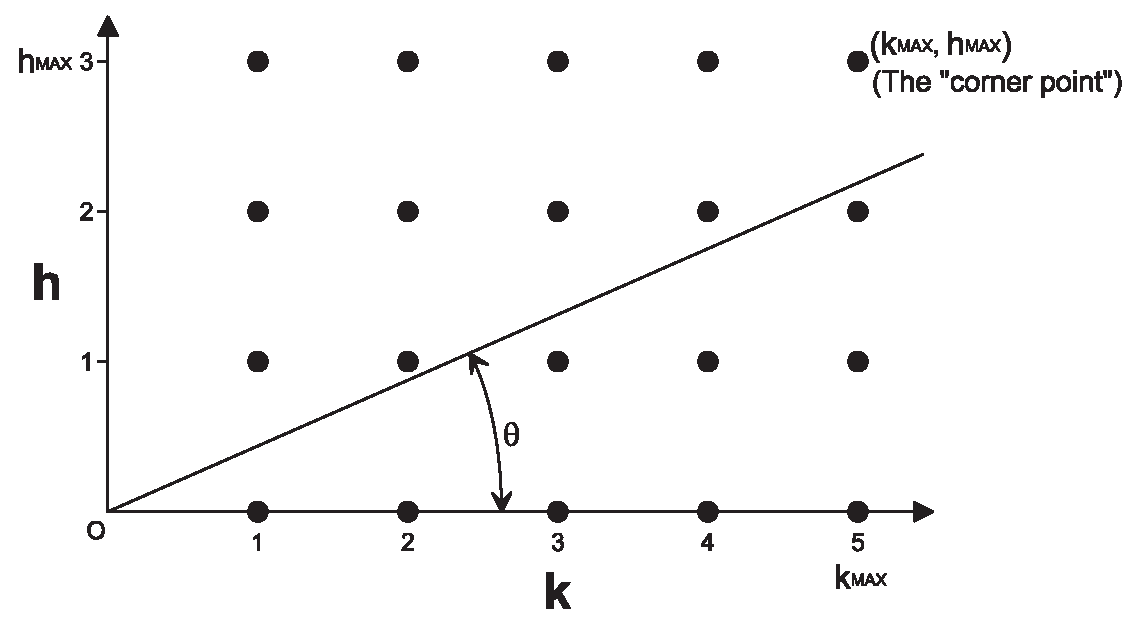
\includegraphics[width=4.6in]{c_rla1/farey01a.eps}
\caption{Graphical Interpretation Of Rational Numbers
         $h/k$ That Can Be Formed With $h \leq h_{MAX}=3$, $k \leq k_{MAX}=5$}
\label{fig:crla1:sfry0:00}
\end{figure}

From the graphical interpretation suggested by Fig.
\ref{fig:crla1:sfry0:00}, the following properties are apparent:

\begin{itemize}
\item The angle of a ray drawn from the origin to the point $(k,h)$
      corresponding to the rational number $h/k$ is $\theta = tan^{-1} \; h/k$.
\item Any integer lattice point on a line from the origin drawn at the
      angle $\theta$ has the value $h/k = tan \; \theta$.  All points
      corresponding to rational numbers with the same value will be on this
      line.
\item A rational number $h/k$ is irreducible if and only if its
      corresponding point $(k,h)$ is directly visible from the origin with
      no intervening points.
\item The Farey series of order $N$, $F_N$, can be formed graphically by
      starting with the set of integer lattice points $(k,h): \; h \in
      \vworkintsetnonneg \wedge 1 \leq k \leq N$, then sweeping a line extended
      from the origin, starting with angle $\theta = 0$, through $0 \leq \theta
      < \pi{}/2$, and recording in order each point directly visible from the
      origin.\footnote{Note that Fig.  \ref{fig:crla1:sfry0:00}, because
      it illustrates the case when $h$ is constrained as well, does not show
      integer lattice points for $h > h_{MAX}$.  If the integer
      lattice shown in Fig.  \ref{fig:crla1:sfry0:00} were extended
      upward, every positive irreducible rational number with
      $k \leq k_{MAX} = 5$ could be found graphically.}
\end{itemize}

Fig.  \ref{fig:crla1:sfry0:01} illustrates the graphical construction
method for $F_5$.  Note that only integer lattice points which are
directly visible from the origin (with no intervening points) are
selected.  (Fig.  \ref{fig:crla1:sfry0:01}, like Fig.
\ref{fig:crla1:sfry0:00}, shows the case of constrained $h$---the integer
lattice should be continued upward to construct $F_5$.)

\begin{figure}
\centering
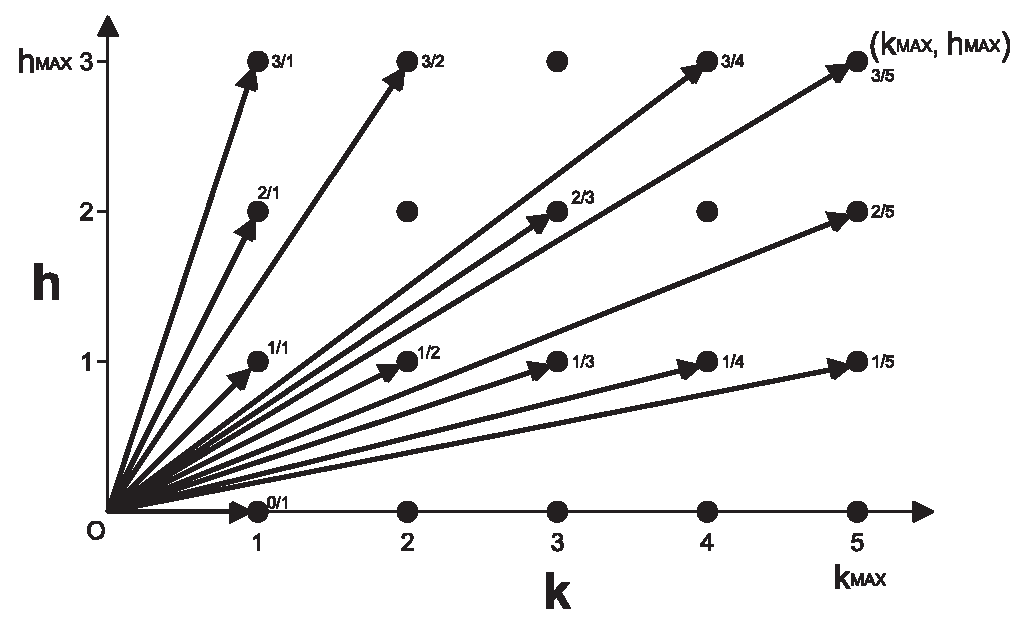
\includegraphics[width=4.6in]{c_rla1/farey01b.eps}
\caption{Graphical Interpretation Of Irreducible Rational Numbers
         $h/k$ That Can Be Formed With $h \leq h_{MAX}=3$, $k \leq k_{MAX}=5$}
\label{fig:crla1:sfry0:01}
\end{figure}

I denote the set of non-negative irreducible rational numbers that can be formed
with $h \leq h_{MAX}$ and $k \leq k_{MAX}$ as $F_{k_{MAX}, h_{MAX}}$\@.
Using this notation, the graphical construction method
depicted in Figure \ref{fig:crla1:sfry0:01} identifies $F_{5,3}$:

\begin{equation}
\label{eq:crla1:sfry0:eq0002a}
F_{5,3}  = \left\{ {\frac{0}{1},\frac{1}{5},\frac{1}{4},
                    \frac{1}{3},\frac{2}{5},\frac{1}{2},
                    \frac{3}{5},\frac{2}{3},\frac{3}{4},
                    \frac{1}{1},\frac{3}{2},\frac{2}{1},
                    \frac{3}{1}} \right\} .
\end{equation}


The ``corner point'' in Figures \ref{fig:crla1:sfry0:00}
and \ref{fig:crla1:sfry0:01}, $k_{MAX}/h_{MAX} = 5/3$, plays a special role:

\begin{itemize}
\item From 0/1 up through the corner point $h_{MAX}/k_{MAX}$,
      the terms are the terms of the Farey series of order
      $k_{MAX}$.
\item From $h_{MAX}/k_{MAX}$ up through $h_{MAX}/1$, the terms
      are the reverse-ordered reciprocals of the terms of the
      Farey series of order $h_{MAX}$\@. (This can be seen
      by transposing the $h$ and $k$ axes of the figures.)
\end{itemize}

The observation about the terms of $F_{5,3}$ that are greater than 3/5 is
important, because it means that if there is a method for finding the
nearest Farey series neighbors to a real number $r_I$ (the case of
only $k$ constrained, $k \leq k_{MAX}$), then there is also a method for finding
the nearest neighbors in $F_{k_{MAX}, h_{MAX}}$ (both $h$ and $k$ constrained).
The method is:

\begin{itemize}
\item If $r_I < k_{MAX}/h_{MAX}$, find the nearest neighbors to $r_I$ in
      $F_{k_{MAX}}$.
\item If $r_I > k_{MAX}/h_{MAX}$, find the nearest neighbors to $1/r_I$
      in $F_{h_{MAX}}$; the reciprocals of those neighbors are the closest
      rational numbers in $F_{k_{MAX}, h_{MAX}}$ to $r_I$.
\end{itemize}

%%%%%%%%%%%%%%%%%%%%%%%%%%%%%%%%%%%%%%%%%%%%%%%%%%%%%%%%%%%%%%%%%%%%%%%%%%%%%%%
%%%%%%%%%%%%%%%%%%%%%%%%%%%%%%%%%%%%%%%%%%%%%%%%%%%%%%%%%%%%%%%%%%%%%%%%%%%%%%%
%%%%%%%%%%%%%%%%%%%%%%%%%%%%%%%%%%%%%%%%%%%%%%%%%%%%%%%%%%%%%%%%%%%%%%%%%%%%%%%
\section{The Continued Fraction Algorithm}
\label{crla1:scfr0}

A \emph{finite simple continued fraction} is a fraction of the form

\begin{equation}
\label{eq:crla1:scfr0:00}
a_0 + \cfrac{1}{a_1 + \cfrac{1}{a_2
    + \cfrac{1}{\;\;\;\;\;\;\;\;\;\;\;\;\;\;\ldots + \cfrac{1}{a_n}}}}
    =
    [a_0; a_1, a_2, \ldots , a_n] ,
\end{equation}

\noindent{}where $a_0 \in \vworkintsetnonneg$ and $a_i \in
\vworkintsetpos$, $i > 0$.  Each integer $a_i$ is called an
\index{continued fraction!element}\emph{element} or \index{continued
fraction!partial quotient}\emph{partial quotient} of the continued
fraction.  To ensure a unique representation, it is required, except in
the case of the continued fraction representation of an integer, that the
final element $a_n$ not be equal to 1.

Continued fractions are unwieldly to write and typeset, so a continued
fraction in the form of (\ref{eq:crla1:scfr0:00}) is written as
$[a_0; a_1, a_2, \ldots , a_n]$.  The separator between $a_0$ and $a_1$ is
a semicolon (`;'), and all other separators are commas (`,').

Continued fractions can be either finite or infinite:

\begin{itemize}
\item A finite continued fraction consists of a finite number of elements
      $[a_0;$ $a_1,$ $a_2,$ $\ldots ,$ $a_n]$\@.  It can be proved that every rational
      number corresponds to a unique finite continued fraction, and that
      every finite continued fraction corresponds to a unique rational number.
\item An infinite continued fraction consists of an infinite number of
      elements $[a_0; a_1, a_2, \ldots]$.  Because every rational number
      corresponds to a finite continued fraction, all irrational numbers have
      infinite continued fraction representations.
\end{itemize}

In engineering work (and due to the general prevalence of computers
and calculators), any $r_I$ to be approximated has a known approximate
numerical value.  Even quantities that are known to be irrational (such
as $\pi$ or $\sqrt{2}$) have a numerical value known to a large number
of significant digits.  For this reason, only the numerical procedure for
obtaining the continued fraction representation of a rational number is
presented (the symbolic procedure is not discussed).  Numerical values
are always rational (for example, 3.1415 is 31,415/10,000).

\index{continued fraction!convergent}The \emph{kth order convergent} of a
continued fraction $[a_0; a_1, \ldots{}, a_n]$ is the irreducible rational
number corresponding to $[a_0; a_1, \ldots{}, a_k]$, $k \leq n$.

An $n$th order continued fraction $[a_0; a_1, \ldots{}, a_n]$ has $n+1$
convergents, $[a_0]$, $[a_0; a_1]$, \ldots{}, and $[a_0; a_1, \ldots{},
a_n]$.  The $k$th order convergent is denoted $s_k$, with numerator $p_k$
and denominator $q_k$.

Algorithm \ref{alg:crla1:scfr0:akgenalg} (below, proof omitted for
brevity) can be used to determine the continued fraction representation
(i.e.  the partial quotients) as well as the convergents of a non-negative
rational number $a/b$\@.

\begin{vworkalgorithmstatementpar}{Continued Fraction Representation and
                                   Convergents of
                                   A Rational Number \mbox{\boldmath $a/b$}}
\label{alg:crla1:scfr0:akgenalg}

\textbf{\emph{Note:}} It is not required that $a/b$ be irreducible.

\begin{alglvl0}
\item $k:=-1$.
\item $divisor_{-1} := a$.
\item $remainder_{-1} := b$.

\item Repeat

\begin{alglvl1}
\item $k := k + 1$.
\item $dividend_k := divisor_{k-1}$.
\item $divisor_k  := remainder_{k-1}$.
\item $a_k :=  dividend_k \; div \; divisor_k$.
\item $remainder_k := dividend_k \; mod \; divisor_k$.
\item If $k=0$, $p_0 = a_0$; else if $k=1$, $p_1 = a_0 a_1 + 1$;
      else $p_i = a_i p_{i-1} + p_{i-2}$.
\item If $k=0$, $q_0 = 1$; else if $k=1$, $q_1 = a_1$;
      else $q_i = a_i q_{i-1} + q_{i-2}$.
\end{alglvl1}

\item Until ($remainder_k = 0$).
\end{alglvl0}
\textbf{\emph{Note:}} The final $s_k = p_k / q_k$ is the irreducible
form of $a/b$.
\end{vworkalgorithmstatementpar}
\vworkalgorithmfooter{}

Convergents have two useful and interesting properties:

\begin{itemize}
\item For each convergent $s_k = p_k/q_k$, there is no rational number
      with a smaller denominator closer to $a/b$\@.\footnote{Table
      \ref{tbl:crla1:sxmp0:01}, part of an example at the end
      of this chapter, provides convergents of $\pi$\@.  It should be
      noted how good the approximations are, even with small denominators,
      due to the average density of rational numbers on the number line\@.
      $s_3$=355/113, for example, has an error on the order of $10^{-7}$\@.
      If this approximation were used to calculate the circumference of the
      earth, the resulting error would be about 11 feet, 2 inches.}
\item Even-ordered convergents are less than $a/b$, and odd-ordered
      convergents are greater than $a/b$; except for the final convergent,
      which is precisely equal to $a/b$.
\end{itemize}

Finally, I present without proof a theorem that indicates how to bracket
a rational number $a/b$ that is not in $F_{k_{MAX}}$ with its two neighbors
in $F_{k_{MAX}}$.

\begin{vworktheoremstatementpar}{Enclosing Neighbors Of \mbox{\boldmath $x \notin F_N$}
                                 In \mbox{\boldmath $F_N$}}
\label{thm:crla1:scfr0:cfenclosingneighbors}
For a non-negative rational
number $a/b$ not in
$F_N$ which has a
continued fraction representation
$[a_0;a_1,a_2,\ldots{} ,a_n]$, the
highest-order convergent $s_k = p_k/q_k$ with $q_k \leq N$ is one
neighbor
to $a/b$ in $F_N$, and the other neighbor in
$F_N$ is

\begin{equation}
\label{eq:crla1:scfr0:thm:cfenclosingneighbors:01}
\frac{{\displaystyle{\left\lfloor {\frac{{N - q_{k - 1} }}{{q_k }}} \right\rfloor}
 p_k  + p_{k - 1} }}{{\displaystyle{\left\lfloor {\frac{{N - q_{k - 1} }}{{q_k }}}
 \right\rfloor} q_k  + q_{k - 1} }}.
\end{equation}
\end{vworktheoremstatementpar}
\begin{vworktheoremproof}
Omitted, as it relies on material not presented for brevity.
\end{vworktheoremproof}
\vworktheoremfooter{}

Theorem \ref{thm:crla1:scfr0:cfenclosingneighbors} can also be applied to
find the Farey neighbors of an $a/b \in F_{k_{MAX}}$.  If
Algorithm \ref{alg:crla1:scfr0:akgenalg} is applied to $a/b$,
(\ref{eq:crla1:scfr0:thm:cfenclosingneighbors:01}) will provide one Farey
neighbor, and (\ref{eq:crla1:sfry0:thm:01:eq01}) through
(\ref{eq:crla1:sfry0:thm:01:eq04}) can be used to provide the other Farey
neighbor\@.  (For brevity, the mathematical basis is not presented.)

Many constants $r_I$ to be approximated are engineering constants based on
measurements or arbitrary conventions, and so are known or accepted to
only a finite number of significant digits.  Such constants are always
rational, and Algorithm \ref{alg:crla1:scfr0:akgenalg} and Theorem
\ref{thm:crla1:scfr0:cfenclosingneighbors} can be applied with no special
consideration.

Some constants, however, are irrational and so have an infinite continued
fraction representation.  The question arises of how to be sure that one
is using enough decimal digits in applying Algorithm
\ref{alg:crla1:scfr0:akgenalg} and Theorem
\ref{thm:crla1:scfr0:cfenclosingneighbors}.  The easiest practical
approach is to confine $r_I$ by an inequality and verify that the Farey
neighbors calculated are the same at both boundaries of the inequality\@.
(It isn't actually necessary to calculate the Farey neighbors to perform
this verification: two rational numbers that have the same highest-order
convergent with $q_k \leq N$ have the same Farey neighbors in $F_N$, but
the \emph{nearest} Farey neighbor may be different for the two rational
numbers.)

Once the two Farey neighbors are calculated, it may be desirable to
determine which is closer to $r_I$.  I'm not aware of a method to do this
other than numerical calculation, although such a method may exist using
higher-order partial quotients or convergents than are used to calculate
the Farey neighbors.


%%%%%%%%%%%%%%%%%%%%%%%%%%%%%%%%%%%%%%%%%%%%%%%%%%%%%%%%%%%%%%%%%%%%%%%%%%%%%%%
%%%%%%%%%%%%%%%%%%%%%%%%%%%%%%%%%%%%%%%%%%%%%%%%%%%%%%%%%%%%%%%%%%%%%%%%%%%%%%%
%%%%%%%%%%%%%%%%%%%%%%%%%%%%%%%%%%%%%%%%%%%%%%%%%%%%%%%%%%%%%%%%%%%%%%%%%%%%%%%
\section{Examples}
\label{crla1:sxmp0}

This section provides examples to illustrate the techniques.

\begin{vworkexamplestatement}
\label{exmp:crla1:sxmp0:01}
Find the best rational approximation to $\pi$ with a denominator not exceeding $2^{24}-1$.
\end{vworkexamplestatement}
\begin{vworkexampleparsection}{Solution} From the problem statement,
$h$ is unconstrained and $k_{MAX}=$16,\-777,\-215.

$2^{24}$ is in the tens of millions (8 digits)\@.  As a crude guess for
how many digits of $\pi$ might lead to unique Farey neighbors for both
ends of an inequality, I will guess 16.

There are numerous websites that provide large numbers of digits of $\pi$\@.
Using 16 digits from a website, one can bound the value of $\pi$:

\begin{equation}
3.141592653589793 < \pi < 3.141592653589794.
\end{equation}

Table \ref{tbl:crla1:sxmp0:01} shows the application of Algorithm
\ref{alg:crla1:scfr0:akgenalg} to find the continued fraction partial
quotients and convergents of $3.141592653589793$\@.  It is only necessary
to continue Algorithm \ref{alg:crla1:scfr0:akgenalg} far enough to establish
the highest-ordered convergent with $q_k \leq k_{MAX}$, and from the table this
is $p_{11}/q_{11}$.

\begin{table}
\caption{Continued Fraction Partial Quotients and Convergents of 3.141592653589793 (Example \ref{exmp:crla1:sxmp0:01})}
\label{tbl:crla1:sxmp0:01}
\begin{center}
\begin{tabular}{|c|c|c|c|c|c|c|}
\hline
\small{Index} & \small{$dividend_k$}      & \small{$divisor_k$}        & \small{$a_k$}   & \small{$remainder_k$}   & \small{$p_k$}      & \small{$q_k$}       \\
\small{($k$)} &                           &                            &                 &                         &                    &                     \\
\hline
\hline
\small{-1}    & \small{N/A}               & \small{3,141,592,}         & \small{N/A}     & \small{1,000,000,}      & \small{N/A}        & \small{N/A}         \\
              &                           & \small{653,589,793}        &                 & \small{000,000,000}     &                    &                     \\
\hline
\small{0}     &  \small{3,141,592}        & \small{1,000,000,}         & \small{3}       & \small{141,592,}        & \small{3}          & \small{1}           \\
              & \small{653,589,793}       & \small{000,000,000}        &                 & \small{653,589,793}     &                    &                     \\
\hline
\small{1}     & \small{1,000,000,}        & \small{141,592,}           & \small{7}       & \small{8,851,}          & \small{22}         & \small{7}           \\
              & \small{000,000,000}       & \small{653,589,793}        &                 & \small{424,871,449}     &                    &                     \\
\hline
\small{2}     & \small{141,592,}          & \small{8,851,}             & \small{15}      & \small{8,821,}          & \small{333}        & \small{106}         \\
              & \small{653,589,793}       & \small{424,871,449}        &                 & \small{280,518,058}     &                    &                     \\
\hline
\small{3}     & \small{8,851,}            & \small{8,821,}             & \small{1}       & \small{30,}             & \small{355}        & \small{113}         \\
              & \small{424,871,449}       & \small{280,518,058}        &                 & \small{144,353,391}     &                    &                     \\
\hline
\small{4}     & \small{8,821,}            & \small{30,}                & \small{292}     & \small{19,}             & \small{103,993}    & \small{33,102}      \\
              & \small{280,518,058}       & \small{144,353,391}        &                 & \small{129,327,886}     &                    &                     \\
\hline
\small{5}     & \small{30,}               & \small{19,}                & \small{1}       & \small{11,}             & \small{104,348}    & \small{33,215}      \\
              & \small{144,353,391}       & \small{129,327,886}        &                 & \small{015,025,505}     &                    &                     \\
\hline
\small{6}     & \small{19,}               & \small{11,}                & \small{1}       & \small{8,}              & \small{208,341}    & \small{66,317}      \\
              & \small{129,327,886}       & \small{015,025,505}        &                 & \small{114,302,381}     &                    &                     \\
\hline
\small{7}     & \small{11,}               & \small{8,}                 & \small{1}       & \small{2,}              & \small{312,689}    & \small{88,532}      \\
              & \small{015,025,505}       & \small{114,302,381}        &                 & \small{900,723,124}     &                    &                     \\
\hline
\small{8}     & \small{8,}                & \small{2,}                 & \small{2}       & \small{2,}              & \small{833,719}    & \small{265,381}     \\
              & \small{114,302,381}       & \small{900,723,124}        &                 & \small{312,856,133}     &                    &                     \\
\hline
\small{9}     & \small{2,}                & \small{2,}                 & \small{1}       & \small{587,866,991}     & \small{1,146,408}  & \small{364,913}     \\
              & \small{900,723,124}       & \small{312,856,133}        &                 &                         &                    &                     \\
\hline
\small{10}    & \small{2,}                & \small{587,866,991}        & \small{3}       & \small{549,255,160}     & \small{4,272,943}  & \small{1,360,120}   \\
              & \small{312,856,133}       &                            &                 &                         &                    &                     \\
\hline
\small{11}    & \small{587,866,991}       & \small{549,255,160}        & \small{1}       & \small{38,611,831}      & \small{5,419,351}  & \small{1,725,033}   \\
\hline
\small{12}    & \small{549,255,160}       & \small{38,611,831}         & \small{14}      & \small{8,689,526}       & \small{80,143,857} & \small{25,510,582}  \\
\hline
\multicolumn{7}{|c|}{\small{Remaining partial quotients and convergents omitted.}} \\
\hline
\end{tabular}
\end{center}
\end{table}

From Theorem \ref{thm:crla1:scfr0:cfenclosingneighbors}, one Farey
neighbor of 3.141592653589793 is

\begin{equation}
s_{11} = \frac{p_{11}}{q_{11}} = \frac{5,\!419,\!351}{1,\!725,\!033} .
\end{equation}

By (\ref{eq:crla1:scfr0:thm:cfenclosingneighbors:01}), the other Farey neighbor is

\begin{eqnarray}
\nonumber{}& \displaystyle{\frac{{\displaystyle{\left\lfloor {\frac{{N - q_{k - 1} }}{{q_k }}} \right\rfloor}
 p_k  + p_{k - 1} }}{{\displaystyle{\left\lfloor {\frac{{N - q_{k - 1} }}{{q_k }}}
 \right\rfloor} q_k  + q_{k - 1} }}}
& \\
& =
\displaystyle{\frac{{\displaystyle{\left\lfloor {\frac{{16,\!777,\!215 - 1,\!360,\!120 }}{{1,\!725,\!033}}} \right\rfloor}
 5,\!419,\!351  + 4,\!272,\!943 }}{{\displaystyle{\left\lfloor {\frac{{16,\!777,\!215 - 1,\!360,\!120 }}{{1,\!725,\!033}}}
 \right\rfloor} 1,\!725,\!033  + 1,\!360,\!120 }}} & \\
\nonumber{}& =
\displaystyle{\frac{\displaystyle{47,\!627,\!751}}{\displaystyle{15,\!160,\!384}}} &
\end{eqnarray}

It can be verified that 3.141592653589794 has the same convergents through
$s_{11} = p_{11}/q_{11}$, so it has the same Farey neighbors as
3.141592653589793\@.  Because $s_{11}$ is an odd-ordered convergent, it is guaranteed to
be greater than $r_I$, establishing the ordering of the Farey neighbors:

\begin{eqnarray}
\nonumber{} & \displaystyle{\frac{47,\!627,\!751}{15,\!160,\!384}} < 3.141592653589793 & \\
            & < \pi < & \\
\nonumber{} & 3.141592653589794 < \displaystyle{\frac{5,\!419,\!351}{1,\!725,\!033}} .
\end{eqnarray}

It can be verified by calculation that the left Farey neighbor is
closer to $\pi$ than the right neighbor, although both are extremely good
approximations (with an error on the order of $10^{-14}$).
\end{vworkexampleparsection}

\begin{vworkexamplestatement}
\label{exmp:crla1:sxmp0:02}
Find the best rational approximation to 1.609344 with a numerator
not exceeding 50,000 and denominator not exceeding
exceeding 60,000.
\end{vworkexamplestatement}
\begin{vworkexampleparsection}{Solution} From the problem statement,
$h_{MAX}=50,\!000$ and $k_{MAX}=60,\!000$.

The corner point (see Fig. \ref{fig:crla1:sfry0:01}, p. \pageref{fig:crla1:sfry0:01})
is $k_{MAX}/h_{MAX} = 1.2$\@.  Since $1.609344 > 1.2$, it is necessary to search
for the Farey neighbors of $1.609344^{-1}$ in $F_{h_{MAX}}$, and the reciprocals
of those neighbors will be the best rational approximations we seek.

Table \ref{tbl:crla1:sxmp0:02} shows the application of Algorithm
\ref{alg:crla1:scfr0:akgenalg} to find the continued fraction partial
quotients and convergents of 1000000/1609344 (the reciprocal of 1.609344).

\begin{table}
\caption{Continued Fraction Partial Quotients and Convergents of $1.609344^{-1}$ (Example \ref{exmp:crla1:sxmp0:02})}
\label{tbl:crla1:sxmp0:02}
\begin{center}
\begin{tabular}{|c|c|c|c|c|c|c|}
\hline
\small{Index} & \small{$dividend_k$}      & \small{$divisor_k$}        & \small{$a_k$}   & \small{$remainder_k$}   & \small{$p_k$}      & \small{$q_k$}       \\
\small{($k$)} &                           &                            &                 &                         &                    &                     \\
\hline
\hline
\small{-1}    & \small{N/A}               & \small{1,000,000}          & \small{N/A}     & \small{1,609.344}       & \small{N/A}        & \small{N/A}         \\
\hline
\small{0}     &  \small{1,000,000}        & \small{1,609344}           & \small{0}       & \small{1,000,000}       & \small{0}          & \small{1}           \\
\hline
\small{1}     & \small{1,609,344,}        & \small{1,000,000}          & \small{1}       & \small{609,344}         & \small{1}          & \small{1}           \\
\hline
\small{2}     & \small{1,000,000}         & \small{609,344}            & \small{1}       & \small{390,656}         & \small{1}          & \small{2}           \\
\hline
\small{3}     & \small{609,344}           & \small{390,656}            & \small{1}       & \small{218,688}         & \small{2}          & \small{3}           \\
\hline
\small{4}     & \small{390,656}           & \small{218,688}            & \small{1}       & \small{171,968}         & \small{3}          & \small{5}           \\
\hline
\small{5}     & \small{218,688}           & \small{171,968}            & \small{1}       & \small{46,720}          & \small{5}          & \small{8}           \\
\hline
\small{6}     & \small{171,968}           & \small{46,720}             & \small{3}       & \small{31,080}          & \small{18}         & \small{29}          \\
\hline
\small{7}     & \small{46,720}            & \small{31,080}             & \small{1}       & \small{14,912}          & \small{23}         & \small{37}          \\
\hline
\small{8}     & \small{31,808}            & \small{14,912}             & \small{2}       & \small{1,984}           & \small{64}         & \small{103}         \\
\hline
\small{9}     & \small{14,912}            & \small{1,984}              & \small{7}       & \small{1,024}           & \small{471}        & \small{758}         \\
\hline
\small{10}    & \small{46,720}            & \small{1,024}              & \small{1}       & \small{960}             & \small{535}        & \small{861}         \\
\hline
\small{11}    & \small{1,024}             & \small{960}                & \small{1}       & \small{64}              & \small{1,006}      & \small{1,619}       \\
\hline
\small{12}    & \small{960}               & \small{64}                 & \small{15}      & \small{0}               & \small{15,625}     & \small{25,146}      \\
\hline
\end{tabular}
\end{center}
\end{table}

Note in Table \ref{tbl:crla1:sxmp0:02} that the final convergent (the reduced
form of 1,000,000/1,609,344), $s_{12} = 15,\!625/25,\!146$, has
$q_{12} < h_{MAX}$, so the reduced form of 1,000,000/1,609,344
is already in $F_{h_{MAX}}$.

It may be helpful to have more choices of a rational number than $1/s_{12}$.  We can use
(\ref{eq:crla1:scfr0:thm:cfenclosingneighbors:01}) to find an adjacent member
of $F_{h_{MAX}}$.  Although $1/s_{12}$ is exactly $r_I$, the same logic mentioned
earlier involving even-numbered and odd-numbered convergents applies.  Even-numbered
convergents (except the final convergent) are less than $r_I$, so the rational number formed by
(\ref{eq:crla1:scfr0:thm:cfenclosingneighbors:01}) will be greater than $s_{12}$.
Applying (\ref{eq:crla1:scfr0:thm:cfenclosingneighbors:01}) yields:

\begin{eqnarray}
\nonumber{}& \displaystyle{\frac{{\displaystyle{\left\lfloor {\frac{{N - q_{k - 1} }}{{q_k }}} \right\rfloor}
 p_k  + p_{k - 1} }}{{\displaystyle{\left\lfloor {\frac{{N - q_{k - 1} }}{{q_k }}}
 \right\rfloor} q_k  + q_{k - 1} }}}
& \\
& =
\displaystyle{\frac{{\displaystyle{\left\lfloor {\frac{{50,\!000 - 1,\!619 }}{{25,\!146}}} \right\rfloor}
 15,\!625  + 1,\!006 }}{{\displaystyle{\left\lfloor {\frac{{50,\!000 - 1,\!619 }}{{25,\!146}}}
 \right\rfloor} 25,\!146  + 1,\!619 }}} & \\
\nonumber{}& =
\displaystyle{\frac{\displaystyle{16,\!631}}{\displaystyle{26,\!765}}} &
\end{eqnarray}

We now have calculated two consecutive terms in $F_{50,\!000}$, $s_{12}$=15,625/25,146 and 16,631/26,765\@.
We can apply (\ref{eq:crla1:sfry0:thm:01:eq03}) and (\ref{eq:crla1:sfry0:thm:01:eq04}) to obtain
the previous term:

\begin{eqnarray}
\nonumber{}h_j  & = & \left\lfloor {\frac{{k_{j + 2}  + N}}{{k_{j + 1} }}}\right\rfloor h_{j + 1}  - h_{j + 2} \\
                & = & \left\lfloor {\frac{{26,\!765  + 50,\!000}}{{25,\!146 }}}\right\rfloor 15,\!625  - 16,\!631 \\
\nonumber{}     & = & 30,\!244
\end{eqnarray}

\begin{eqnarray}
\nonumber{}k_j  & = & \left\lfloor {\frac{{k_{j + 2}  + N}}{{k_{j + 1} }}}\right\rfloor k_{j + 1}  - k_{j + 2} \\
                & = & \left\lfloor {\frac{{26,\!765  + 50,\!000}}{{25,\!146 }}}\right\rfloor 25,\!146  - 26,\!765 \\
\nonumber{}     & = & 48,\!673
\end{eqnarray}

We have determined three consecutive terms of $F_{50,\!000}$:

\begin{equation}
F_{50,\!000} = \left\{ \ldots, \frac{30,\!244}{48,\!673},
\frac{15,\!625}{25,\!146} = s_{12} = 1.609344^{-1},
\frac{16,\!631}{26,\!765}, \ldots \right\}.
\end{equation}

If we take the reciprocals of the terms and reverse the order, we also have determined
three consecutive terms of $F_{50,\!000,60,\!000}$:

\begin{equation}
\label{eq:crla1:sxmp0:02:01}
F_{50,\!000,60,\!000} = \left\{ \ldots, \frac{26,\!765}{16,\!631},
\frac{25,\!146}{15,\!625} = s_{12}^{-1} = 1.609344,
\frac{48,\!673}{30,\!244}, \ldots \right\}.
\end{equation}

All three of the approximations in (\ref{eq:crla1:sxmp0:02:01}) are quite
good.  For most applications, the exact value $r_I = 1/s_{12} =
25,\!146/15,\!625$ would be used.  However, even in the case where $r_I$
can be represented exactly under the constraints, it is possible to
determine neighboring rational approximations.
\end{vworkexampleparsection}



% Chapter: Coding Theory
\chapter{Coding Theory}
\label{ccth0}

%%%%%%%%%%%%%%%%%%%%%%%%%%%%%%%%%%%%%%%%%%%%%%%%%%%%%%%%%%%%%%%%%%%%%%%%%%%%%%%
%%%%%%%%%%%%%%%%%%%%%%%%%%%%%%%%%%%%%%%%%%%%%%%%%%%%%%%%%%%%%%%%%%%%%%%%%%%%%%%
%%%%%%%%%%%%%%%%%%%%%%%%%%%%%%%%%%%%%%%%%%%%%%%%%%%%%%%%%%%%%%%%%%%%%%%%%%%%%%%
\section{Introduction and Overview}
\label{ccth0:siov0}

TBD.



% Chapter: Non-Numerical Algorithms
\chapter{Non-Numerical Algorithms}
\label{cnna0}

%%%%%%%%%%%%%%%%%%%%%%%%%%%%%%%%%%%%%%%%%%%%%%%%%%%%%%%%%%%%%%%%%%%%%%%%%%%%%%%
%%%%%%%%%%%%%%%%%%%%%%%%%%%%%%%%%%%%%%%%%%%%%%%%%%%%%%%%%%%%%%%%%%%%%%%%%%%%%%%
%%%%%%%%%%%%%%%%%%%%%%%%%%%%%%%%%%%%%%%%%%%%%%%%%%%%%%%%%%%%%%%%%%%%%%%%%%%%%%%
\section{Introduction and Overview}
\label{cnna0:siov0}

TBD.



% Chapter: Integer Arithmetic Algorithms and Implementation
\chapter{Integer Arithmetic Algorithms and Implementation}        
\label{caal0}

%%%%%%%%%%%%%%%%%%%%%%%%%%%%%%%%%%%%%%%%%%%%%%%%%%%%%%%%%%%%%%%%%%%%%%%%%%%%%%%
%%%%%%%%%%%%%%%%%%%%%%%%%%%%%%%%%%%%%%%%%%%%%%%%%%%%%%%%%%%%%%%%%%%%%%%%%%%%%%%
%%%%%%%%%%%%%%%%%%%%%%%%%%%%%%%%%%%%%%%%%%%%%%%%%%%%%%%%%%%%%%%%%%%%%%%%%%%%%%%
\section{Introduction}
\label{caal0:sint0}

TBD.




% Chapter: Integer Mathematical Algorithms and Implementation
\chapter{Integer Mathematical Algorithms and Implementation}        
\label{cmal0}

%%%%%%%%%%%%%%%%%%%%%%%%%%%%%%%%%%%%%%%%%%%%%%%%%%%%%%%%%%%%%%%%%%%%%%%%%%%%%%%
%%%%%%%%%%%%%%%%%%%%%%%%%%%%%%%%%%%%%%%%%%%%%%%%%%%%%%%%%%%%%%%%%%%%%%%%%%%%%%%
%%%%%%%%%%%%%%%%%%%%%%%%%%%%%%%%%%%%%%%%%%%%%%%%%%%%%%%%%%%%%%%%%%%%%%%%%%%%%%%
\section{Introduction}
\label{cmal0:sint0}

TBD.




% Chapter: Fixed-Point Arithmetic Algorithms and Implementation
\chapter{Fixed-Point Arithmetic Algorithms and Implementation}        
\label{caal2}

%%%%%%%%%%%%%%%%%%%%%%%%%%%%%%%%%%%%%%%%%%%%%%%%%%%%%%%%%%%%%%%%%%%%%%%%%%%%%%%
%%%%%%%%%%%%%%%%%%%%%%%%%%%%%%%%%%%%%%%%%%%%%%%%%%%%%%%%%%%%%%%%%%%%%%%%%%%%%%%
%%%%%%%%%%%%%%%%%%%%%%%%%%%%%%%%%%%%%%%%%%%%%%%%%%%%%%%%%%%%%%%%%%%%%%%%%%%%%%%
\section{Introduction}
\label{caal2:sint0}

TBD.




% Chapter: Fixed-Point Mathematical Algorithms and Implementation
\chapter{Fixed-Point Mathematical Algorithms and Implementation}        
\label{cmal2}

%%%%%%%%%%%%%%%%%%%%%%%%%%%%%%%%%%%%%%%%%%%%%%%%%%%%%%%%%%%%%%%%%%%%%%%%%%%%%%%
%%%%%%%%%%%%%%%%%%%%%%%%%%%%%%%%%%%%%%%%%%%%%%%%%%%%%%%%%%%%%%%%%%%%%%%%%%%%%%%
%%%%%%%%%%%%%%%%%%%%%%%%%%%%%%%%%%%%%%%%%%%%%%%%%%%%%%%%%%%%%%%%%%%%%%%%%%%%%%%
\section{Introduction}
\label{cmal2:sint0}

TBD.




% Chapter: Real and Floating-Point Arithmetic Algorithms and Implementation
\chapter{Real and Floating-Point Arithmetic Algorithms and Implementation}        
\label{craa0}

%%%%%%%%%%%%%%%%%%%%%%%%%%%%%%%%%%%%%%%%%%%%%%%%%%%%%%%%%%%%%%%%%%%%%%%%%%%%%%%
%%%%%%%%%%%%%%%%%%%%%%%%%%%%%%%%%%%%%%%%%%%%%%%%%%%%%%%%%%%%%%%%%%%%%%%%%%%%%%%
%%%%%%%%%%%%%%%%%%%%%%%%%%%%%%%%%%%%%%%%%%%%%%%%%%%%%%%%%%%%%%%%%%%%%%%%%%%%%%%
\section{Introduction}
\label{craa0:sint0}

TBD.




% Chapter: Real and Floating-Point Mathematical Algorithms and Implementation
\chapter{Real and Floating-Point Mathematical Algorithms and Implementation}        
\label{crma0}

%%%%%%%%%%%%%%%%%%%%%%%%%%%%%%%%%%%%%%%%%%%%%%%%%%%%%%%%%%%%%%%%%%%%%%%%%%%%%%%
%%%%%%%%%%%%%%%%%%%%%%%%%%%%%%%%%%%%%%%%%%%%%%%%%%%%%%%%%%%%%%%%%%%%%%%%%%%%%%%
%%%%%%%%%%%%%%%%%%%%%%%%%%%%%%%%%%%%%%%%%%%%%%%%%%%%%%%%%%%%%%%%%%%%%%%%%%%%%%%
\section{Introduction}
\label{crma0:sint0}

TBD.




% Chapter: Linear Filters and Control System Elements
\chapter{Linear Filters and Control System Elements}
\label{clfc0}

%%%%%%%%%%%%%%%%%%%%%%%%%%%%%%%%%%%%%%%%%%%%%%%%%%%%%%%%%%%%%%%%%%%%%%%%%%%%%%%
%%%%%%%%%%%%%%%%%%%%%%%%%%%%%%%%%%%%%%%%%%%%%%%%%%%%%%%%%%%%%%%%%%%%%%%%%%%%%%%
%%%%%%%%%%%%%%%%%%%%%%%%%%%%%%%%%%%%%%%%%%%%%%%%%%%%%%%%%%%%%%%%%%%%%%%%%%%%%%%
\section{Introduction and Overview}
\label{clfc0:siov0}

TBD.



% Chapter: Non-Linear Filters and Debouncing
\chapter{Non-Linear Filters and Debouncing}
\label{cnlf0}

%%%%%%%%%%%%%%%%%%%%%%%%%%%%%%%%%%%%%%%%%%%%%%%%%%%%%%%%%%%%%%%%%%%%%%%%%%%%%%%
%%%%%%%%%%%%%%%%%%%%%%%%%%%%%%%%%%%%%%%%%%%%%%%%%%%%%%%%%%%%%%%%%%%%%%%%%%%%%%%
%%%%%%%%%%%%%%%%%%%%%%%%%%%%%%%%%%%%%%%%%%%%%%%%%%%%%%%%%%%%%%%%%%%%%%%%%%%%%%%
\section{Introduction and Overview}
\label{cnlf0:siov0}

TBD.



% Chapter: Random and Pseudo-Random Number Generation
\chapter{Random and Pseudo-Random Number Generation}
\label{crng0}

%%%%%%%%%%%%%%%%%%%%%%%%%%%%%%%%%%%%%%%%%%%%%%%%%%%%%%%%%%%%%%%%%%%%%%%%%%%%%%%
%%%%%%%%%%%%%%%%%%%%%%%%%%%%%%%%%%%%%%%%%%%%%%%%%%%%%%%%%%%%%%%%%%%%%%%%%%%%%%%
%%%%%%%%%%%%%%%%%%%%%%%%%%%%%%%%%%%%%%%%%%%%%%%%%%%%%%%%%%%%%%%%%%%%%%%%%%%%%%%
\section{Introduction and Overview}
\label{crng0:siov0}

TBD.



% Chapter: Non-Cryptographic Hashes
\chapter{Non-Cryptographic Hashes}
\label{cnch0}

%%%%%%%%%%%%%%%%%%%%%%%%%%%%%%%%%%%%%%%%%%%%%%%%%%%%%%%%%%%%%%%%%%%%%%%%%%%%%%%
%%%%%%%%%%%%%%%%%%%%%%%%%%%%%%%%%%%%%%%%%%%%%%%%%%%%%%%%%%%%%%%%%%%%%%%%%%%%%%%
%%%%%%%%%%%%%%%%%%%%%%%%%%%%%%%%%%%%%%%%%%%%%%%%%%%%%%%%%%%%%%%%%%%%%%%%%%%%%%%
\section{Introduction and Overview}
\label{cnch0:siov0}

TBD.



% Chapter: Cryptographic Hashes
\chapter{Cryptographic Hashes}
\label{cchs0}

%%%%%%%%%%%%%%%%%%%%%%%%%%%%%%%%%%%%%%%%%%%%%%%%%%%%%%%%%%%%%%%%%%%%%%%%%%%%%%%
%%%%%%%%%%%%%%%%%%%%%%%%%%%%%%%%%%%%%%%%%%%%%%%%%%%%%%%%%%%%%%%%%%%%%%%%%%%%%%%
%%%%%%%%%%%%%%%%%%%%%%%%%%%%%%%%%%%%%%%%%%%%%%%%%%%%%%%%%%%%%%%%%%%%%%%%%%%%%%%
\section{Introduction and Overview}
\label{cchs0:siov0}

TBD.



% Chapter: Symmetric-Key Ciphers and Algorithms
\chapter{Symmetric-Key Ciphers and Algorithms}
\label{cskc0}

%%%%%%%%%%%%%%%%%%%%%%%%%%%%%%%%%%%%%%%%%%%%%%%%%%%%%%%%%%%%%%%%%%%%%%%%%%%%%%%
%%%%%%%%%%%%%%%%%%%%%%%%%%%%%%%%%%%%%%%%%%%%%%%%%%%%%%%%%%%%%%%%%%%%%%%%%%%%%%%
%%%%%%%%%%%%%%%%%%%%%%%%%%%%%%%%%%%%%%%%%%%%%%%%%%%%%%%%%%%%%%%%%%%%%%%%%%%%%%%
\section{Introduction and Overview}
\label{cskc0:siov0}

TBD.



% Chapter: Asymmetric-Key Ciphers and Algorithms
\chapter{Asymmetric-Key Ciphers and Algorithms}
\label{cakc0}

%%%%%%%%%%%%%%%%%%%%%%%%%%%%%%%%%%%%%%%%%%%%%%%%%%%%%%%%%%%%%%%%%%%%%%%%%%%%%%%
%%%%%%%%%%%%%%%%%%%%%%%%%%%%%%%%%%%%%%%%%%%%%%%%%%%%%%%%%%%%%%%%%%%%%%%%%%%%%%%
%%%%%%%%%%%%%%%%%%%%%%%%%%%%%%%%%%%%%%%%%%%%%%%%%%%%%%%%%%%%%%%%%%%%%%%%%%%%%%%
\section{Introduction and Overview}
\label{cakc0:siov0}

TBD.



% Chapter: Miscellaneous Mathematical and Algorithmic Topics
\chapter{Miscellaneous Mathematical and Algorithmic Topics}
\label{cmat0}

%%%%%%%%%%%%%%%%%%%%%%%%%%%%%%%%%%%%%%%%%%%%%%%%%%%%%%%%%%%%%%%%%%%%%%%%%%%%%%%
%%%%%%%%%%%%%%%%%%%%%%%%%%%%%%%%%%%%%%%%%%%%%%%%%%%%%%%%%%%%%%%%%%%%%%%%%%%%%%%
%%%%%%%%%%%%%%%%%%%%%%%%%%%%%%%%%%%%%%%%%%%%%%%%%%%%%%%%%%%%%%%%%%%%%%%%%%%%%%%
\section{Introduction and Overview}
\label{cmat0:siov0}

TBD.



% Part: Library Documentation
\part{Library Documentation}

% Chapter: How to Use NumLib
\chapter{How to Use \emph{\productbasenameshort{}}}
\label{cuuc0}


%%%%%%%%%%%%%%%%%%%%%%%%%%%%%%%%%%%%%%%%%%%%%%%%%%%%%%%%%%%%%%%%%%%%%%%%%%%%%%%
%%%%%%%%%%%%%%%%%%%%%%%%%%%%%%%%%%%%%%%%%%%%%%%%%%%%%%%%%%%%%%%%%%%%%%%%%%%%%%%
%%%%%%%%%%%%%%%%%%%%%%%%%%%%%%%%%%%%%%%%%%%%%%%%%%%%%%%%%%%%%%%%%%%%%%%%%%%%%%%
\section{Introduction and Overview}
\label{cuuc0:siov0}

TBD.




% Chapter: Utility and Miscellaneous Functions
\chapter{Utility and Miscellaneous Functions}
\label{cnef0}

%%%%%%%%%%%%%%%%%%%%%%%%%%%%%%%%%%%%%%%%%%%%%%%%%%%%%%%%%%%%%%%%%%%%%%%%%%%%%%%
%%%%%%%%%%%%%%%%%%%%%%%%%%%%%%%%%%%%%%%%%%%%%%%%%%%%%%%%%%%%%%%%%%%%%%%%%%%%%%%
%%%%%%%%%%%%%%%%%%%%%%%%%%%%%%%%%%%%%%%%%%%%%%%%%%%%%%%%%%%%%%%%%%%%%%%%%%%%%%%
\section{Introduction and Overview}
\label{cnef0:siov0}

TBD.



% Chapter: Block Memory Functions
\chapter{Block Memory Functions}
\label{cbmf0}

%%%%%%%%%%%%%%%%%%%%%%%%%%%%%%%%%%%%%%%%%%%%%%%%%%%%%%%%%%%%%%%%%%%%%%%%%%%%%%%
%%%%%%%%%%%%%%%%%%%%%%%%%%%%%%%%%%%%%%%%%%%%%%%%%%%%%%%%%%%%%%%%%%%%%%%%%%%%%%%
%%%%%%%%%%%%%%%%%%%%%%%%%%%%%%%%%%%%%%%%%%%%%%%%%%%%%%%%%%%%%%%%%%%%%%%%%%%%%%%
\section{Introduction and Overview}
\label{cbmf0:siov0}

TBD.



% Chapter: Search Functions
\chapter{Search Functions}
\label{csea0}

%%%%%%%%%%%%%%%%%%%%%%%%%%%%%%%%%%%%%%%%%%%%%%%%%%%%%%%%%%%%%%%%%%%%%%%%%%%%%%%
%%%%%%%%%%%%%%%%%%%%%%%%%%%%%%%%%%%%%%%%%%%%%%%%%%%%%%%%%%%%%%%%%%%%%%%%%%%%%%%
%%%%%%%%%%%%%%%%%%%%%%%%%%%%%%%%%%%%%%%%%%%%%%%%%%%%%%%%%%%%%%%%%%%%%%%%%%%%%%%
\section{Introduction and Overview}
\label{csea0:siov0}

TBD.



% Chapter: Sort Functions
\chapter[Sort Functions]
        {Sort Functions}
\chaptermark{Sort Functions}        

\label{csol0}

%%%%%%%%%%%%%%%%%%%%%%%%%%%%%%%%%%%%%%%%%%%%%%%%%%%%%%%%%%%%%%%%%%%%%%%%%%%%%%%
%%%%%%%%%%%%%%%%%%%%%%%%%%%%%%%%%%%%%%%%%%%%%%%%%%%%%%%%%%%%%%%%%%%%%%%%%%%%%%%
%%%%%%%%%%%%%%%%%%%%%%%%%%%%%%%%%%%%%%%%%%%%%%%%%%%%%%%%%%%%%%%%%%%%%%%%%%%%%%%
\section{Introduction and Overview}
\label{csol0:siov0}

TBD.



% Chapter: Array Manipulation Functions
\chapter{Array Manipulation Functions}
\label{cami0}


%%%%%%%%%%%%%%%%%%%%%%%%%%%%%%%%%%%%%%%%%%%%%%%%%%%%%%%%%%%%%%%%%%%%%%%%%%%%%%%
%%%%%%%%%%%%%%%%%%%%%%%%%%%%%%%%%%%%%%%%%%%%%%%%%%%%%%%%%%%%%%%%%%%%%%%%%%%%%%%
%%%%%%%%%%%%%%%%%%%%%%%%%%%%%%%%%%%%%%%%%%%%%%%%%%%%%%%%%%%%%%%%%%%%%%%%%%%%%%%
\section{Introduction and Overview}
\label{cami0:siov0}

TBD.



%% Chapter: Bit-Mapped Set Functions
\chapter{Bit-Mapped Set Functions}        
\label{cbsf0}

%%%%%%%%%%%%%%%%%%%%%%%%%%%%%%%%%%%%%%%%%%%%%%%%%%%%%%%%%%%%%%%%%%%%%%%%%%%%%%%
%%%%%%%%%%%%%%%%%%%%%%%%%%%%%%%%%%%%%%%%%%%%%%%%%%%%%%%%%%%%%%%%%%%%%%%%%%%%%%%
%%%%%%%%%%%%%%%%%%%%%%%%%%%%%%%%%%%%%%%%%%%%%%%%%%%%%%%%%%%%%%%%%%%%%%%%%%%%%%%
\section{Introduction and Overview}
\label{cbsf0:siov0}

TBD.





% Chapter: Vertical Counter Functions
\chapter{Vertical Counter Functions}
\label{cvco0}

%%%%%%%%%%%%%%%%%%%%%%%%%%%%%%%%%%%%%%%%%%%%%%%%%%%%%%%%%%%%%%%%%%%%%%%%%%%%%%%
%%%%%%%%%%%%%%%%%%%%%%%%%%%%%%%%%%%%%%%%%%%%%%%%%%%%%%%%%%%%%%%%%%%%%%%%%%%%%%%
%%%%%%%%%%%%%%%%%%%%%%%%%%%%%%%%%%%%%%%%%%%%%%%%%%%%%%%%%%%%%%%%%%%%%%%%%%%%%%%
\section{Introduction and Overview}
\label{cvco0:siov0}

TBD.



% Chapter: Native Data Type Integer Utility and Arithmetic Functions
\chapter{Native Data Type Integer Utility and Arithmetic Functions}
\label{cafn0}

%%%%%%%%%%%%%%%%%%%%%%%%%%%%%%%%%%%%%%%%%%%%%%%%%%%%%%%%%%%%%%%%%%%%%%%%%%%%%%%
%%%%%%%%%%%%%%%%%%%%%%%%%%%%%%%%%%%%%%%%%%%%%%%%%%%%%%%%%%%%%%%%%%%%%%%%%%%%%%%
%%%%%%%%%%%%%%%%%%%%%%%%%%%%%%%%%%%%%%%%%%%%%%%%%%%%%%%%%%%%%%%%%%%%%%%%%%%%%%%
\section{Introduction and Overview}
\label{cafn0:siov0}



% Chapter: Native Data Type Integer Mathematical Functions
\chapter{Native Data Type Integer Mathematical Functions}
\label{cbaf0}

%%%%%%%%%%%%%%%%%%%%%%%%%%%%%%%%%%%%%%%%%%%%%%%%%%%%%%%%%%%%%%%%%%%%%%%%%%%%%%%
%%%%%%%%%%%%%%%%%%%%%%%%%%%%%%%%%%%%%%%%%%%%%%%%%%%%%%%%%%%%%%%%%%%%%%%%%%%%%%%
%%%%%%%%%%%%%%%%%%%%%%%%%%%%%%%%%%%%%%%%%%%%%%%%%%%%%%%%%%%%%%%%%%%%%%%%%%%%%%%
\section{Introduction and Overview}
\label{cbaf0:siov0}

TBD.




% Chapter: Native Data Type Fixed-Point Utility and Arithmetic Functions
\chapter{Native Data Type Fixed-Point Utility and Arithmetic Functions}
\label{cfpa0}

%%%%%%%%%%%%%%%%%%%%%%%%%%%%%%%%%%%%%%%%%%%%%%%%%%%%%%%%%%%%%%%%%%%%%%%%%%%%%%%
%%%%%%%%%%%%%%%%%%%%%%%%%%%%%%%%%%%%%%%%%%%%%%%%%%%%%%%%%%%%%%%%%%%%%%%%%%%%%%%
%%%%%%%%%%%%%%%%%%%%%%%%%%%%%%%%%%%%%%%%%%%%%%%%%%%%%%%%%%%%%%%%%%%%%%%%%%%%%%%
\section{Introduction and Overview}
\label{cfpa0:siov0}

TBD.




% Chapter: Native Data Type Fixed-Point Mathematical Functions
\chapter{Native Data Type Fixed-Point Mathematical Functions}
\label{cfpa1}

%%%%%%%%%%%%%%%%%%%%%%%%%%%%%%%%%%%%%%%%%%%%%%%%%%%%%%%%%%%%%%%%%%%%%%%%%%%%%%%
%%%%%%%%%%%%%%%%%%%%%%%%%%%%%%%%%%%%%%%%%%%%%%%%%%%%%%%%%%%%%%%%%%%%%%%%%%%%%%%
%%%%%%%%%%%%%%%%%%%%%%%%%%%%%%%%%%%%%%%%%%%%%%%%%%%%%%%%%%%%%%%%%%%%%%%%%%%%%%%
\section{Introduction and Overview}
\label{cfpa1:siov0}

TBD.



% Chapter: Native Data Type Floating-Point Utility and Arithmetic Functions
\chapter{Native Data Type Floating-Point Utility and Arithmetic Functions}
\label{caal1}

%%%%%%%%%%%%%%%%%%%%%%%%%%%%%%%%%%%%%%%%%%%%%%%%%%%%%%%%%%%%%%%%%%%%%%%%%%%%%%%
%%%%%%%%%%%%%%%%%%%%%%%%%%%%%%%%%%%%%%%%%%%%%%%%%%%%%%%%%%%%%%%%%%%%%%%%%%%%%%%
%%%%%%%%%%%%%%%%%%%%%%%%%%%%%%%%%%%%%%%%%%%%%%%%%%%%%%%%%%%%%%%%%%%%%%%%%%%%%%%
\section{Introduction and Overview}
\label{caal1:siov0}

TBD.



% Chapter: Native Data Type Floating-Point Mathematical Functions
\chapter{Native Data Type Floating-Point Mathematical Functions}
\label{cafn1}

%%%%%%%%%%%%%%%%%%%%%%%%%%%%%%%%%%%%%%%%%%%%%%%%%%%%%%%%%%%%%%%%%%%%%%%%%%%%%%%
%%%%%%%%%%%%%%%%%%%%%%%%%%%%%%%%%%%%%%%%%%%%%%%%%%%%%%%%%%%%%%%%%%%%%%%%%%%%%%%
%%%%%%%%%%%%%%%%%%%%%%%%%%%%%%%%%%%%%%%%%%%%%%%%%%%%%%%%%%%%%%%%%%%%%%%%%%%%%%%
\section{Introduction and Overview}
\label{cafn1:siov0}

TBD.



% Chapter: Large Integer Utility and Arithmetic Functions
\chapter[Large Integer Utility and Arithmetic Functions]
        {Large Integer Utility and Arithmetic Functions}

\chaptermark{Large Integer Utility and Arithmetic Functions}

\label{claf0}

%%%%%%%%%%%%%%%%%%%%%%%%%%%%%%%%%%%%%%%%%%%%%%%%%%%%%%%%%%%%%%%%%%%%%%%%%%%%%%%
%%%%%%%%%%%%%%%%%%%%%%%%%%%%%%%%%%%%%%%%%%%%%%%%%%%%%%%%%%%%%%%%%%%%%%%%%%%%%%%
%%%%%%%%%%%%%%%%%%%%%%%%%%%%%%%%%%%%%%%%%%%%%%%%%%%%%%%%%%%%%%%%%%%%%%%%%%%%%%%
\section{Introduction and Overview}
\label{claf0:siov0}

TBD.



% Chapter: Large Integer Mathematical Functions
\chapter[Large Integer Mathematical Functions]
        {Large Integer Mathematical Functions}

\chaptermark{Large Integer Mathematical Functions}

\label{claf1}

%%%%%%%%%%%%%%%%%%%%%%%%%%%%%%%%%%%%%%%%%%%%%%%%%%%%%%%%%%%%%%%%%%%%%%%%%%%%%%%
%%%%%%%%%%%%%%%%%%%%%%%%%%%%%%%%%%%%%%%%%%%%%%%%%%%%%%%%%%%%%%%%%%%%%%%%%%%%%%%
%%%%%%%%%%%%%%%%%%%%%%%%%%%%%%%%%%%%%%%%%%%%%%%%%%%%%%%%%%%%%%%%%%%%%%%%%%%%%%%
\section{Introduction and Overview}
\label{claf1:siov0}

TBD.



% Chapter: Large Fixed-Point Utility and Arithmetic Functions
\chapter{Large Fixed-Point Utility and Arithmetic Functions}
\label{cfpa2}

%%%%%%%%%%%%%%%%%%%%%%%%%%%%%%%%%%%%%%%%%%%%%%%%%%%%%%%%%%%%%%%%%%%%%%%%%%%%%%%
%%%%%%%%%%%%%%%%%%%%%%%%%%%%%%%%%%%%%%%%%%%%%%%%%%%%%%%%%%%%%%%%%%%%%%%%%%%%%%%
%%%%%%%%%%%%%%%%%%%%%%%%%%%%%%%%%%%%%%%%%%%%%%%%%%%%%%%%%%%%%%%%%%%%%%%%%%%%%%%
\section{Introduction and Overview}
\label{cfpa2:siov0}

TBD.




% Chapter: Large Fixed-Point Mathematical Functions
\chapter{Large Fixed-Point Mathematical Functions}
\label{cfpa3}

%%%%%%%%%%%%%%%%%%%%%%%%%%%%%%%%%%%%%%%%%%%%%%%%%%%%%%%%%%%%%%%%%%%%%%%%%%%%%%%
%%%%%%%%%%%%%%%%%%%%%%%%%%%%%%%%%%%%%%%%%%%%%%%%%%%%%%%%%%%%%%%%%%%%%%%%%%%%%%%
%%%%%%%%%%%%%%%%%%%%%%%%%%%%%%%%%%%%%%%%%%%%%%%%%%%%%%%%%%%%%%%%%%%%%%%%%%%%%%%
\section{Introduction and Overview}
\label{cfpa3:siov0}

TBD.



% Chapter: Large Floating-Point Utility and Arithmetic Functions
\chapter[Large Floating-Point Utility and Arithmetic Functions]
        {Large Floating-Point Utility and Arithmetic Functions}

\chaptermark{Large Floating-Point Utility and Arithmetic Functions}

\label{claf2}

%%%%%%%%%%%%%%%%%%%%%%%%%%%%%%%%%%%%%%%%%%%%%%%%%%%%%%%%%%%%%%%%%%%%%%%%%%%%%%%
%%%%%%%%%%%%%%%%%%%%%%%%%%%%%%%%%%%%%%%%%%%%%%%%%%%%%%%%%%%%%%%%%%%%%%%%%%%%%%%
%%%%%%%%%%%%%%%%%%%%%%%%%%%%%%%%%%%%%%%%%%%%%%%%%%%%%%%%%%%%%%%%%%%%%%%%%%%%%%%
\section{Introduction and Overview}
\label{claf2:siov0}

TBD.



% Chapter: Large Floating-Point Mathematical Functions
\chapter[Large Floating-Point Mathematical Functions]
        {Large Floating-Point Mathematical Functions}

\chaptermark{Large Integer Mathematical Functions}

\label{claf3}

%%%%%%%%%%%%%%%%%%%%%%%%%%%%%%%%%%%%%%%%%%%%%%%%%%%%%%%%%%%%%%%%%%%%%%%%%%%%%%%
%%%%%%%%%%%%%%%%%%%%%%%%%%%%%%%%%%%%%%%%%%%%%%%%%%%%%%%%%%%%%%%%%%%%%%%%%%%%%%%
%%%%%%%%%%%%%%%%%%%%%%%%%%%%%%%%%%%%%%%%%%%%%%%%%%%%%%%%%%%%%%%%%%%%%%%%%%%%%%%
\section{Introduction and Overview}
\label{claf3:siov0}

TBD.



% Chapter: Linear Filter Functions
\chapter{Linear Filter and Control System Element Functions}
\label{clfi0}

%%%%%%%%%%%%%%%%%%%%%%%%%%%%%%%%%%%%%%%%%%%%%%%%%%%%%%%%%%%%%%%%%%%%%%%%%%%%%%%
%%%%%%%%%%%%%%%%%%%%%%%%%%%%%%%%%%%%%%%%%%%%%%%%%%%%%%%%%%%%%%%%%%%%%%%%%%%%%%%
%%%%%%%%%%%%%%%%%%%%%%%%%%%%%%%%%%%%%%%%%%%%%%%%%%%%%%%%%%%%%%%%%%%%%%%%%%%%%%%
\section{Introduction and Overview}
\label{clfi0:siov0}

TBD.




% Chapter: Non-Linear Filter Functions
\chapter{Non-Linear Filter Functions}
\label{cnfi0}


%%%%%%%%%%%%%%%%%%%%%%%%%%%%%%%%%%%%%%%%%%%%%%%%%%%%%%%%%%%%%%%%%%%%%%%%%%%%%%%
%%%%%%%%%%%%%%%%%%%%%%%%%%%%%%%%%%%%%%%%%%%%%%%%%%%%%%%%%%%%%%%%%%%%%%%%%%%%%%%
%%%%%%%%%%%%%%%%%%%%%%%%%%%%%%%%%%%%%%%%%%%%%%%%%%%%%%%%%%%%%%%%%%%%%%%%%%%%%%%
\section{Introduction and Overview}
\label{cnfi0:siov0}

TBD.



% Chapter: Pseudo-Random Number Generation Functions
\chapter{Pseudo-Random Number Generation Functions}
\label{crng1}

%%%%%%%%%%%%%%%%%%%%%%%%%%%%%%%%%%%%%%%%%%%%%%%%%%%%%%%%%%%%%%%%%%%%%%%%%%%%%%%
%%%%%%%%%%%%%%%%%%%%%%%%%%%%%%%%%%%%%%%%%%%%%%%%%%%%%%%%%%%%%%%%%%%%%%%%%%%%%%%
%%%%%%%%%%%%%%%%%%%%%%%%%%%%%%%%%%%%%%%%%%%%%%%%%%%%%%%%%%%%%%%%%%%%%%%%%%%%%%%
\section{Introduction and Overview}
\label{crng1:siov0}

TBD.



% Chapter: Non-Cryptographic Hash Functions
\chapter[Non-Cryptographic Hash Functions]
        {Non-Cryptographic Hash Functions}
\chaptermark{Non-Cryptographic Hash Functions}        
\label{ccrc0}

%%%%%%%%%%%%%%%%%%%%%%%%%%%%%%%%%%%%%%%%%%%%%%%%%%%%%%%%%%%%%%%%%%%%%%%%%%%%%%%
%%%%%%%%%%%%%%%%%%%%%%%%%%%%%%%%%%%%%%%%%%%%%%%%%%%%%%%%%%%%%%%%%%%%%%%%%%%%%%%
%%%%%%%%%%%%%%%%%%%%%%%%%%%%%%%%%%%%%%%%%%%%%%%%%%%%%%%%%%%%%%%%%%%%%%%%%%%%%%%
\section{Introduction and Overview}
\label{ccrc0:siov0}

TBD.



% Chapter: Cryptographic Hash Functions
\chapter{Cryptographic Hash Functions}
\label{ccrh0}

%%%%%%%%%%%%%%%%%%%%%%%%%%%%%%%%%%%%%%%%%%%%%%%%%%%%%%%%%%%%%%%%%%%%%%%%%%%%%%%
%%%%%%%%%%%%%%%%%%%%%%%%%%%%%%%%%%%%%%%%%%%%%%%%%%%%%%%%%%%%%%%%%%%%%%%%%%%%%%%
%%%%%%%%%%%%%%%%%%%%%%%%%%%%%%%%%%%%%%%%%%%%%%%%%%%%%%%%%%%%%%%%%%%%%%%%%%%%%%%
\section{Introduction and Overview}
\label{ccrh0:siov0}

TBD.



% Chapter: Symmetric Cipher Functions
\chapter{Symmetric Cipher Functions}
\label{ccip0}

%%%%%%%%%%%%%%%%%%%%%%%%%%%%%%%%%%%%%%%%%%%%%%%%%%%%%%%%%%%%%%%%%%%%%%%%%%%%%%%
%%%%%%%%%%%%%%%%%%%%%%%%%%%%%%%%%%%%%%%%%%%%%%%%%%%%%%%%%%%%%%%%%%%%%%%%%%%%%%%
%%%%%%%%%%%%%%%%%%%%%%%%%%%%%%%%%%%%%%%%%%%%%%%%%%%%%%%%%%%%%%%%%%%%%%%%%%%%%%%
\section{Introduction and Overview}
\label{ccip0:siov0}

TBD.



% Chapter: Asymmetric Cipher Functions
\chapter{Asymmetric Cipher Functions}
\label{ccip1}

%%%%%%%%%%%%%%%%%%%%%%%%%%%%%%%%%%%%%%%%%%%%%%%%%%%%%%%%%%%%%%%%%%%%%%%%%%%%%%%
%%%%%%%%%%%%%%%%%%%%%%%%%%%%%%%%%%%%%%%%%%%%%%%%%%%%%%%%%%%%%%%%%%%%%%%%%%%%%%%
%%%%%%%%%%%%%%%%%%%%%%%%%%%%%%%%%%%%%%%%%%%%%%%%%%%%%%%%%%%%%%%%%%%%%%%%%%%%%%%
\section{Introduction and Overview}
\label{ccip1:siov0}

TBD.



% Part: Developer and Contributor Information
\part{Developer and Contributor Information}

% Chapter: Library Development and Modification Procedures
\chapter{Library Development and Modification Procedures}
\label{cbpc0}


%%%%%%%%%%%%%%%%%%%%%%%%%%%%%%%%%%%%%%%%%%%%%%%%%%%%%%%%%%%%%%%%%%%%%%%%%%%%%%%
%%%%%%%%%%%%%%%%%%%%%%%%%%%%%%%%%%%%%%%%%%%%%%%%%%%%%%%%%%%%%%%%%%%%%%%%%%%%%%%
%%%%%%%%%%%%%%%%%%%%%%%%%%%%%%%%%%%%%%%%%%%%%%%%%%%%%%%%%%%%%%%%%%%%%%%%%%%%%%%
\section{Generating Library Source Code from Templates}
\label{cbpc0:sgsc0}

TBD.





% Part: Appendices, Bibliography, and Index 
\part{Appendices, Bibliography, and Index}

%Mark the start of appendices.  This causes numbering to be with letters
%instead of numbers.
\appendix

%Glossary of Terms
\chapter{Glossary Of Terms}
\markboth{GLOSSARY OF TERMS}{GLOSSARY OF TERMS}

\label{cglo0}

\begin{vworktermglossaryenum}


\item \index{set!cardinality}\textbf{cardinality}

      The number of elements in a set, denoted $n( \cdot )$. 
      \emph{Example:} $n( \{ 12 , 29 , 327 \} ) = 3$.  

\item \index{coprime}\textbf{coprime}

      Having no prime factors in common.
      \emph{Example:} 6 and 7 are coprime, whereas 6 and 8 are not coprime.  


\end{vworktermglossaryenum}


%
%Glossary of Mathematical Notation
\chapter{Glossary Of Mathematical And Other Notation}
\markboth{GLOSSARY OF MATHEMATICAL NOTATION}{GLOSSARY OF MATHEMATICAL NOTATION}
\label{cglo1}

%%%%%%%%%%%%%%%%%%%%%%%%%%%%%%%%%%%%%%%%%%%%%%%%%%%%%%%%%%%%%%%%%%%%%%%%%%%%%%%
%%%%%%%%%%%%%%%%%%%%%%%%%%%%%%%%%%%%%%%%%%%%%%%%%%%%%%%%%%%%%%%%%%%%%%%%%%%%%%%
%%%%%%%%%%%%%%%%%%%%%%%%%%%%%%%%%%%%%%%%%%%%%%%%%%%%%%%%%%%%%%%%%%%%%%%%%%%%%%%

\section*{General}

\begin{vworkmathtermglossaryenum}

\item \index{divides}%
      \mbox{\boldmath $ \vworkdivides $}

      $a \vworkdivides b$, 
      read ``\emph{$a$ divides $b$}'', denotes that $b/a$ has no remainder.
      Equivalently,
      $(a \vworkdivides b) \Rightarrow (\exists c \in \vworkintset{}, b = ac)$.

\item \index{divides}%
      \mbox{\boldmath $ \vworknotdivides $}

      $a \vworknotdivides b$, 
      read ``\emph{$a$ does not divide $b$}'', denotes that $b/a$ has a reminder.
      Equivalently,
      $(a \vworknotdivides b) \Rightarrow (\nexists c \in \vworkintset{}, b = ac)$.

\item \index{floor function}%
      \mbox{\boldmath $ \lfloor \cdot \rfloor $}

      The \emph{floor} function.  $\lfloor x \rfloor$ is the largest
      integer not larger than $x$.

\item \index{ceiling function}%
      \mbox{\boldmath $\lceil \cdot \rceil$ }

      The \emph{ceiling} function.
      $\lceil x \rceil$
      is the smallest integer not smaller than $x$.
\end{vworkmathtermglossaryenum}

%%%%%%%%%%%%%%%%%%%%%%%%%%%%%%%%%%%%%%%%%%%%%%%%%%%%%%%%%%%%%%%%%%%%%%%%%%%%%%%
%%%%%%%%%%%%%%%%%%%%%%%%%%%%%%%%%%%%%%%%%%%%%%%%%%%%%%%%%%%%%%%%%%%%%%%%%%%%%%%
%%%%%%%%%%%%%%%%%%%%%%%%%%%%%%%%%%%%%%%%%%%%%%%%%%%%%%%%%%%%%%%%%%%%%%%%%%%%%%%
%
%\section*{Usage Of English And Greek Letters}
%
%\begin{vworkmathtermglossaryenum}
%
%\item \mbox {\boldmath $a/b$}
%
%      An arbitrary \index{rational number}rational number.
%
%\item \mbox {\boldmath $ F_N $}
%
%      The \index{Farey series}Farey 
%      series of order $N$.  The Farey series is the
%      ordered set of irreducible rational numbers 
%          in [0,1] with a
%      denominator not larger than $N$.
%
%\item \mbox {\boldmath $F_{k_{MAX}, \overline{h_{MAX}}}$}
%      
%          \index{FKMAXHMAX@$F_{k_{MAX}, \overline{h_{MAX}}}$}
%          The ordered set of irreducible rational numbers
%          $h/k$ subject to the constraints $0 \leq h \leq h_{MAX}$
%          and $1 \leq k \leq h_{MAX}$.  
%%         (See Section \cfryzeroxrefhyphen{}\ref{cfry0:schk0}.)
%
%
%\item \mbox{\boldmath $H/K$}, \mbox{\boldmath $h/k$},
%      \mbox{\boldmath $h'/k'$}, \mbox{\boldmath $h''/k''$},
%      \mbox{\boldmath $h_i/k_i$}
%
%      Terms in a Farey series of order $N$.
%
%\item \mbox{\boldmath $r_A$}
%
%      The rational number $h/k$ used to approximate
%      an arbitrary real number $r_I$.
%
%\item \mbox{\boldmath $r_I$}
%
%      The real number, which may or may not be rational,
%      which is to be approximated by a rational number
%      $r_A = h/k$.
%
%\item \textbf{reduced}
%
%      See \emph{irreducible}.
%
%\item \mbox{\boldmath $s_k = p_k/q_k$}
%
%      The $k$th convergent of a continued fraction.
%
%\item \mbox{\boldmath $x_{MAX}$}
%
%      The largest element of the domain for which the
%      behavior of an approximation must be guaranteed.
%      In this paper, most derivations assume
%      that $x \in [0, x_{MAX}]$, $x_{MAX} \in \vworkintsetpos{}$.
%\end{vworkmathtermglossaryenum}

%%%%%%%%%%%%%%%%%%%%%%%%%%%%%%%%%%%%%%%%%%%%%%%%%%%%%%%%%%%%%%%%%%%%%%%%%%%%%%%
%%%%%%%%%%%%%%%%%%%%%%%%%%%%%%%%%%%%%%%%%%%%%%%%%%%%%%%%%%%%%%%%%%%%%%%%%%%%%%%
%%%%%%%%%%%%%%%%%%%%%%%%%%%%%%%%%%%%%%%%%%%%%%%%%%%%%%%%%%%%%%%%%%%%%%%%%%%%%%%

%\section*{Bitfields And Portions Of Integers}
%
%\begin{vworkmathtermglossaryenum}
%\item \mbox{\boldmath $a_{b}$}
%
%      The $b$th bit of the integer $a$.  Bits are numbered with the
%      least significant bit ``0'', and consecutively through 
%      ``$n-1$'', where $n$ is the total number of bits.
%
%      In general, if $p$ is an $n$-bit unsigned integer,
%
%      \begin{equation}
%      \nonumber p = \sum_{i=0}^{n-1} 2^i p_i .
%      \end{equation}
%
%\item \mbox{\boldmath $a_{c:b}$}
%
%      The integer consisting of the $b$th through the
%      $c$th bits of the integer $a$.  Bits are numbered with the
%      least significant bit ``0'', and consecutively through 
%      ``$n-1$'', where $n$ is the total number of bits.
%
%      For example, if $p$ is a 24-bit unsigned integer, then
%
%      \begin{equation}
%      \nonumber p = 2^{16}p_{23:16} + 2^{8}p_{15:8} + p_{7:0} .
%      \end{equation}
%
%\item \mbox{\boldmath $a_{[b]}$}
%
%      The $b$th word of the integer $a$.  Words are numbered 
%      with the
%      least significant word ``0'', and consecutively through 
%      ``$n-1$'', where $n$ is the total number of words.
%
%      In general, if $p$ is an $n$-word unsigned integer 
%      and $z$ is the wordsize in bits,
%
%      \begin{equation}
%      \nonumber p = \sum_{i=0}^{n-1} 2^{iz} p_i .
%      \end{equation}
%
%\item \mbox{\boldmath $a_{[c:b]}$}
%
%      The integer consisting of the $b$th through the
%      $c$th word of the integer $a$.  Words are numbered with the
%      least significant word ``0'', and consecutively through 
%      ``$n-1$'', where $n$ is the total number of words.
%
%      For example, if $p$ is a 24-word unsigned integer and
%      $z$ is the wordsize in bits, then
%
%      \begin{equation}
%      \nonumber p = 2^{16z}p_{[23:16]} + 2^{8z}p_{[15:8]} + p_{[7:0]} .
%      \end{equation}
%
%\end{vworkmathtermglossaryenum}

%%%%%%%%%%%%%%%%%%%%%%%%%%%%%%%%%%%%%%%%%%%%%%%%%%%%%%%%%%%%%%%%%%%%%%%%%%%%%%%
%%%%%%%%%%%%%%%%%%%%%%%%%%%%%%%%%%%%%%%%%%%%%%%%%%%%%%%%%%%%%%%%%%%%%%%%%%%%%%%
%%%%%%%%%%%%%%%%%%%%%%%%%%%%%%%%%%%%%%%%%%%%%%%%%%%%%%%%%%%%%%%%%%%%%%%%%%%%%%%

%\section*{Matrices And Vectors}
%
%\begin{vworkmathtermglossaryenum}
%
%\item \mbox{\boldmath $0$}
%
%      $\mathbf{0}$ (in bold face) is used to denote either a vector or matrix
%      populated with all zeroes.  Optionally, in cases where the context is not clear
%      or where there is cause to highlight the dimension, $\mathbf{0}$ may be subscripted
%      to indicate the dimension, i.e. 
%      
%      \begin{equation}
%      \nonumber
%      \mathbf{0}_3 = \left[\begin{array}{c} 0 \\ 0 \\ 0 \end{array}\right]
%      \end{equation}
%
%      \begin{equation}
%      \nonumber
%      \mathbf{0}_{3 \times 2} = \left[\begin{array}{cc} 0&0 \\ 0&0 \\ 0&0 \end{array}\right]
%      \end{equation}
%
%\item \mbox{\boldmath $I$}
%
%      $I$ is used to denote the square identity matrix (the matrix with all
%      elements 0 except elements on the diagonal which are 1).
%      Optionally, in cases where the context is not clear
%      or where there is cause to highlight the dimension, $I$ may be subscripted
%      to indicate the dimension, i.e. 
%      
%      \begin{equation}
%      \nonumber
%      I = I_3 = I_{3 \times 3} = \left[\begin{array}{ccc} 1&0&0 \\ 0&1&0 \\ 0&0&1 \end{array}\right]
%      \end{equation}
%
%\end{vworkmathtermglossaryenum}


%%%%%%%%%%%%%%%%%%%%%%%%%%%%%%%%%%%%%%%%%%%%%%%%%%%%%%%%%%%%%%%%%%%%%%%%%%%%%%%
%%%%%%%%%%%%%%%%%%%%%%%%%%%%%%%%%%%%%%%%%%%%%%%%%%%%%%%%%%%%%%%%%%%%%%%%%%%%%%%
%%%%%%%%%%%%%%%%%%%%%%%%%%%%%%%%%%%%%%%%%%%%%%%%%%%%%%%%%%%%%%%%%%%%%%%%%%%%%%%

\section*{Sets}

\begin{vworkmathtermglossaryenum}

\item \index{set!cardinality}\mbox{\boldmath $n( \cdot )$}

      The \emph{cardinality} of a set (the
      number of elements in the set).

\end{vworkmathtermglossaryenum}

%%%%%%%%%%%%%%%%%%%%%%%%%%%%%%%%%%%%%%%%%%%%%%%%%%%%%%%%%%%%%%%%%%%%%%%%%%%%%%%
%%%%%%%%%%%%%%%%%%%%%%%%%%%%%%%%%%%%%%%%%%%%%%%%%%%%%%%%%%%%%%%%%%%%%%%%%%%%%%%
%%%%%%%%%%%%%%%%%%%%%%%%%%%%%%%%%%%%%%%%%%%%%%%%%%%%%%%%%%%%%%%%%%%%%%%%%%%%%%%

%\section*{Sets Of Numbers}
%
%\begin{vworkmathtermglossaryenum}
%
%\item \mbox{\boldmath $\vworkintsetpos$}
%
%      The 
%      \index{natural number}
%      \index{N@$\vworkintsetpos$}
%      set of positive integers (natural numbers).
%
%\item \mbox{\boldmath $\vworkratset$}
%
%      The 
%      \index{rational number}
%      \index{Q@$\vworkratset$}
%      set of rational numbers.
%
%\item \mbox{\boldmath $\vworkratsetnonneg$}
%
%      The 
%      \index{rational number}
%      \index{Q+@$\vworkratsetnonneg$}
%      set of non-negative rational numbers.
%
%\item \mbox{\boldmath $\vworkrealset$}
%
%      The 
%      \index{real number}
%      \index{R@$\vworkrealset$}
%      set of real numbers.
%
%\item \mbox{\boldmath $\vworkrealsetnonneg$}
%
%      The 
%      \index{real number}
%      \index{R+@$\vworkrealsetnonneg$}
%      set of non-negative real numbers.
%
%\item \mbox{\boldmath $\vworkintset$}
%
%      The 
%      \index{integer}
%      \index{Z@$\vworkintset$}
%      set of integers.
%
%\item \mbox{\boldmath $\vworkintsetnonneg$}
%
%      The 
%      \index{integer}
%      \index{Z+@$\vworkintsetnonneg$}
%      set of non-negative integers.
%
%\end{vworkmathtermglossaryenum}


%
%Bibliography
\cleardoublepage
\addcontentsline{toc}{chapter}{Bibliography}
%Legend
%    b - book
%    c - company
%    d - document
%    i - individual, i.e. person
%    n - newsgroup
%    p - paper
%    s - software, software distributions
%    w - web page.
%
%%%%%%%%%%%%%%%%%%%%%%%%%%%%%%%%%%%%%%%%%%%%%%%%%%%%%%%%%%%%%%%%%%%%%%%%%%
\chapter*{Bibliography}

\markboth{BIBLIOGRAPHY}{BIBLIOGRAPHY}

\newcounter{custombibcounter}

\nocite{*}

%%%%%%%%%%%%%%%%%%%%%%%%%%%%%%%%%%%%%%%%%%%%%%%%%%%%%%%%%%%%%%%%%%%%%%%%%%
%
%\section*{Two-Factor Authentication Vendors}
%\index{two-factor authentication}
%
%\begin{thecustombibliography}{9999}
%
%\bibitem{bibref:c:cryptocardcorporation}
%CryptoCard Corporation,\index{CryptoCard Corporation}\\
%\texttt{http://www.cryptocard.com}
%
%\end{thecustombibliography}
%
%
%%%%%%%%%%%%%%%%%%%%%%%%%%%%%%%%%%%%%%%%%%%%%%%%%%%%%%%%%%%%%%%%%%%%%%%%%%
%
%\section*{Corporations and Organizations}
%
%\begin{thecustombibliography}{9999}
%
%\bibitem{bibref:c:cosmicsoftware}
%Cosmic Software\index{Cosmic Software}\\
%\texttt{http://www.cosmic-us.com}
%
%\end{thecustombibliography}
%
%%%%%%%%%%%%%%%%%%%%%%%%%%%%%%%%%%%%%%%%%%%%%%%%%%%%%%%%%%%%%%%%%%%%%%%%%%

%\section*{Individuals}
%
%\begin{thecustombibliography}{9999}
%
%\bibitem{bibref:i:davidtashley}
%David T. Ashley,\index{Ashley, David T.}
%E-mail: \texttt{dashley@gmail.com}
%
%\bibitem{bibref:i:johnbibo}
%John Bibo,\index{Bibo, John}
%E-mail: \texttt{jbibo@cosmic-us.com}
%
%\bibitem{bibref:i:mikeburns}
%Michael Burns,\index{Burns, Michael}
%E-mail: \texttt{mjb@cosmic-us.com}
%
%\end{thecustombibliography}

%%%%%%%%%%%%%%%%%%%%%%%%%%%%%%%%%%%%%%%%%%%%%%%%%%%%%%%%%%%%%%%%%%%%%%%%%%


%\subsection*{Mathematical Philosophy Books}
%
%\begin{thecustombibliography}{9999}
%
%\bibitem{bibref:b:mathematiciansapology:1940}
%G. H. Hardy,
%\newblock{\em A Mathematician's Apology}, ISBN 0-521-42706-1 (Paperback),
%Cambridge University Press.
%
%\end{thecustombibliography}

%%%%%%%%%%%%%%%%%%%%%%%%%%%%%%%%%%%%%%%%%%%%%%%%%%%%%%%%%%%%%%%%%%%%%%%%%%

%\subsection*{Mathematicians (Amateur And Professional)}
%
%\begin{thecustombibliography}{9999}
%
%\bibitem{bibref:i:davideppstein}
%David Eppstein,\index{Eppstein, David}
%E-mail: \texttt{eppstein@ics.uci.edu}
%
%\end{thecustombibliography}

%%%%%%%%%%%%%%%%%%%%%%%%%%%%%%%%%%%%%%%%%%%%%%%%%%%%%%%%%%%%%%%%%%%%%%%%%%

\section*{Books}

\begin{thecustombibliography}{9999}
%
\bibitem{bibref:b:LamportLaTeX}
\index{Lamport, Leslie}\index{LaTeX@\emph{\LaTeX{}}}Leslie Lamport,
\newblock{\em \LaTeX{}: A Document Preparation System},
Addison-Wesley, 1994, 1985; ISBN 0-201-52983-1.

\bibitem{bibref:b:TaocpVolume2}
\index{Knuth, Donald E.}Donald E. Knuth,
\newblock{\em The Art of Computer Programming, Third Edition, Volume 2 / Seminumerical Algorithms},
Addison-Wesley, 1997; ISBN 0-201-89684-2.
%
%\bibitem{bibref:b:KhinchinClassic}
%A. Ya. Khinchin, \index{Khinchin, A. Ya.}
%\newblock{\em Continued Fractions}, University Of
%Chicago Press, 1964; Library Of Congress Catalog Card
%Number 64-15819.
%
%\bibitem{bibref:b:OldsClassic}
%C. D. Olds,
%\newblock{\em Continued Fractions},
%Randam House, 1963,
%Library Of Congress Catalog Card Number 61-12185.
%
\end{thecustombibliography}

%%%%%%%%%%%%%%%%%%%%%%%%%%%%%%%%%%%%%%%%%%%%%%%%%%%%%%%%%%%%%%%%%%%%%%%%%%
\section*{Individuals}


%%%%%%%%%%%%%%%%%%%%%%%%%%%%%%%%%%%%%%%%%%%%%%%%%%%%%%%%%%%%%%%%%%%%%%%%%%

\section*{Websites and Web Pages}

\begin{thecustombibliography}{9999}

\bibitem{bibref:w:gmplibhomepage}
\index{GMP Library@\emph{GMP Library}}GMP Library Home Page,
\texttt{https://gmplib.org/}

\bibitem{bibref:w:miktexhomepage}
\index{MiKTeX@\emph{MiK\TeX{}}}\emph{MiK\TeX{}} Home Page,
\texttt{https://miktex.org/}

\bibitem{bibref:w:wikipedialowpassfilter}
\index{low-pass filter}Low-Pass Filter,
\texttt{http://en.wikipedia.org/wiki/Low-pass\_filter}

\end{thecustombibliography}


%
%Index Must Be Formed At This Directory Level
\cleardoublepage
\addcontentsline{toc}{chapter}{Index}
\printindex
%
\end{document}

%================================================================================
%The information below is from https://www.texfaq.org/FAQ-runheadtoobig.  I'm
%keeping it here because this situation comes up frequently.
%--------------------------------------------------------------------------------
%My section title is too wide for the page header
%--------------------------------------------------------------------------------
%By default, LaTeX sectioning commands make the chapter or section title
%available for use by page headers and the like. Page headers operate in a rather
%constrained area, and it�s common for titles too be too big to fit: the LaTeX
%sectioning commands therefore take an optional argument:
%
%\section[short title]{full title}
%
%If the �short title� is present, it is used both for the table of contents and
%for the page heading. The usual answer to people who complain that their title
%is too big for the running head is to suggest that they the optional argument.
%
%However, using the same text for the table of contents as for the running head
%may also be unsatisfactory: if your chapter titles are seriously long (like those
%of a Victorian novel), a valid and rational scheme is to have a shortened table
%of contents entry, and a really terse entry in the running head.
%
%One of the problems is the tendency of page headings to be set in capitals
%(which take up more space); so why not set headings as written for �ordinary�
%reading? It�s not possible to do so with unmodified LaTeX, but the fancyhdr
%package provides a command \nouppercase for use in its header (and footer)
%lines to suppress LaTeX�s uppercasing tendencies. Classes in the KOMA-script
%bundle don�t uppercase in the first place.
%
%In fact, the sectioning commands use �mark� commands to pass information to the
%page headers. For example, \chapter uses \chaptermark, \section uses
%\sectionmark, and so on. With this knowledge, one can achieve a three-layer
%structure for chapters:
%
%\chapter[middling version]{verbose version}
%\chaptermark{terse version}
%
%which should supply the needs of every taste.
%
%Chapters, however, have it easy: hardly any book design puts a page header on
%a chapter start page. In the case of sections, one has typically to take account
%of the nature of the \*mark commands: the thing that goes in the heading is the
%first mark on the page (or, failing any mark, the last mark on any previous
%page). As a result the recipe for sections is more tiresome:
%
%\section[middling version]{verbose version%
%              \sectionmark{terse version}}
%\sectionmark{terse version}
%
%(the first \sectionmark deals with the header of the page the \section command
%falls on, and the second deal with subsequent pages; note that here, you need the 
%ptional argument to \section, even if �middling version� is in fact the same text
%as �long version�.)
%
%A similar arrangement is necessary even for chapters if the class you�re using is
%odd enough that it puts a page header on a chapter�s opening page.
%
%Note that the titlesec package manages the running heads in a completely different
%fashion; for example, you can use the optional argument of sectioning commands
%for page headers, only, by loading the package as:
%
%\usepackage[toctitles]{titlesec}
%
%The package documentation offers other useful techniques in this area.
%
%The memoir class avoids all the silliness by providing an extra optional
%argument for chapter and sectioning commands, for example:
%
%\section[middling version][terse version]{verbose version}
%
%As a result, it is always possible for users of memoir to tailor the header text to
%fit, with very little trouble.
%================================================================================
%It was discovered that using \index{key@value} entries within footnotes is
%if "value" is formatted.  An additional space was inserted in the .idx file,
%causing the index entry generated from within a footnote to be different than
%the others (and to be listed separately in the index).
%
%Here is the original problematic text:
%    I define \index{limb size}\emph{limb size}\footnote{The terms \emph{limb} 
%    and \emph{limb size} come from \index{GMP Library@\emph{GMP Library}}%
%    \emph{The GMP Library} \cite{bibref:w:gmplibhomepage}.} as the 
%    number of bits in what Knuth calls $w$ (from the quote above).  In 
%
%Here is the line in the .idx file with the extra space:
%    \indexentry{GMP Library@\emph  {GMP Library}}{8}
%
%Here is a web page that describes the problem and a possible workaround.  (My
%workaround, for now is not to use index entries in footnotes.  A second workaround
%might to be to put the \index entry with the footnoted text, rolling the dice that
%the footnote will end up on the same page as the referring number, which it usually
%does.)
%    https://tex.stackexchange.com/questions/145309/index-in-footnode-different-from-index-in-main-text
%
%Here is the most meaningful text from the URL above (in case it disappears):
%    The problem is that \index tries hard not to tokenize its argument too
%    early; but when the \index command appears in the argument to another
%    command (in this case \footnote, the tokenization has already been done.)
%    Thus in the .idx file you get two non matching entries, one with
%
%        @\textit{De Malignitate Erodoti}!
%
%    and the other one with
%
%        @\textit  {De Malignitate Erodoti}!
%
%    A workaround is to always tokenize:
%
%        \newcommand{\indexp}[1]{\index[p]{#1}}
%
%    and using \indexp instead of \index[p].
%================================================================================

